% To compile, use: latexmk -pvc -lualatex dissertation -latexoption="--shell-escape"
%\documentclass[draft,12pt]{nddiss2e}
% \documentclass[final,12pt]{nddiss2e}
\documentclass[noinfo,final,nonatbib]{nddiss2e}
% \usepackage{showframe}
\usepackage{mdframed}
\usepackage{colortbl}
\usepackage{amssymb}
\usepackage{afterpage}
\usepackage{bigdelim}
\usepackage{listings}
\usepackage{makecell}
\usepackage{microtype}
\usepackage{multirow}
\usepackage{newunicodechar}
\usepackage{pgfplots}
\usepackage{pgfplotstable}
\usepackage{physics}
\usepackage{polyglossia}
\usepackage{minted}
\surroundwithmdframed[linewidth=2pt]{minted}
\usepackage[
  type={CC},
  modifier={by-sa},
  version={4.0},
]{doclicense}

\let\abs\relax
\usepackage{siunitx}

\usepackage[noabbrev,nameinlink,capitalize]{cleveref}
\usepackage{caption}
\usepackage{subcaption}
\captionsetup[subfigure]{subrefformat=simple,labelformat=simple}
    \renewcommand\thesubfigure{(\alph{subfigure})}

\usepackage[flushleft]{threeparttablex}
\usepackage{tikz}
\usepackage[compat=1.1.0]{tikz-feynman}
\usepackage{tabulary}
\newcolumntype{Y}{>{\centering\arraybackslash}X}
\newcolumntype{K}[1]{>{\centering\arraybackslash}p{#1}}
\newcolumntype{L}[1]{>{\raggedright\let\newline\\\arraybackslash\hspace{0pt}}m{#1}}
\newcolumntype{C}[1]{>{\centering\let\newline\\\arraybackslash\hspace{0pt}}m{#1}}
\newcolumntype{R}[1]{>{\raggedleft\let\newline\\\arraybackslash\hspace{0pt}}m{#1}}
\newcolumntype{Z}{>{\raggedleft\let\newline\\\arraybackslash\hspace{0pt}}X}
\usepackage{xpatch}
\usepackage[subtle]{savetrees}
\AtBeginDocument{\thinmuskip = 3mu}

\usepackage[disable]{todonotes}
\usepackage{accents}
\usepackage{csquotes}
\usepackage{unicode-math}

\lstset{
  basicstyle=\ttfamily,
}

\sisetup{
  range-phrase=--,
  range-units=single,
  group-minimum-digits=4,
  multi-part-units=single,
  separate-uncertainty,
	table-number-alignment=center,
}
\interfootnotelinepenalty=10000
\usetikzlibrary{arrows,calc,fit,positioning,shapes}

\usepackage{mathtools}
\usepackage{autonum} % only number labeled equations
\DeclarePairedDelimiter{\abs}{\lvert}{\rvert}

\overfullrule=0pt
\usepackage[giveninits=true,isbn=false,sorting=none]{biblatex}

\AtEveryBibitem{%
  \clearlist{language}%
  \ifentrytype{book}{\clearfield{url}}{}%
  \clearlist{abstract}%
  \clearfield{eprintclass}%
  \clearfield{note}
}
\DeclareFieldFormat{labelnumberwidth}{#1\adddot}
% \DeclareFieldFormat{url}{\printtext{URL}\space\href{#1}{\nolinkurl{#1}}}
% \DeclareFieldFormat{doi}{\printtext{DOI}\addcolon\space\href{http://dx.doi.org/#1}{\nolinkurl{#1}}}
\DeclareFieldFormat{shorturl}{\nolinkurl{#1}}
\DeclareFieldFormat{url}{%
  \href{#1}{\printfield{shorturl}}}
\DeclareFieldFormat{doi}{\href{http://dx.doi.org/#1}{\nolinkurl{doi:#1}}}
\DeclareFieldFormat{eprint:arxiv}{%
  \ifhyperref
    {\href{http://arxiv.org/abs/#1}{%
       \nolinkurl{arxiv:#1}%
       \iffieldundef{eprintclass}
         {}
         {\addspace\texttt{\mkbibbrackets{\thefield{eprintclass}}}}}}
    {\nolinkurl{arxiv:#1}
     \iffieldundef{eprintclass}
       {}
       {\addspace\texttt{\mkbibbrackets{\thefield{eprintclass}}}}}}
\setcounter{biburllcpenalty}{9000}
\setcounter{biburlucpenalty}{9000}
\setcounter{biburlnumpenalty}{9000}
\setlength\bibitemsep{\baselineskip}

\renewbibmacro*{in:}{%
  \printtext{%
    \bibstring{In}\intitlepunct}}
\renewbibmacro*{doi+eprint+url}{%
  \iftoggle{bbx:url}
    {\iffieldundef{doi}{\usebibmacro{url+urldate}}{}}
    {}%
  \newunit\newblock
  \iftoggle{bbx:eprint}
    {\iffieldundef{doi}{\usebibmacro{eprint}}{}}
    {}%
  \newunit\newblock
  \iftoggle{bbx:doi}
    {\printfield{doi}}
    {}}

\addbibresource{dissertation.bib}

% Remove the abstract.
\DeclareSourcemap{
  \maps[datatype=bibtex]{
    \map[overwrite=true]{
      \step[fieldset=abstract, null]
    }
    \map[overwrite=true]{
      \step[fieldsource=url]
      \step[fieldset=shorturl, origfieldval]
      \step[fieldsource=shorturl, match=\regexp{https?://}, replace={}]
    }
  }
}

\DeclareDocumentCommand\Pe{}{\ensuremath{e}\xspace}
\DeclareDocumentCommand\Pp{}{\ensuremath{\text{p}}\xspace}
\DeclareDocumentCommand\Pg{}{\ensuremath{\text{g}}\xspace}
\DeclareDocumentCommand\Pnu{}{\ensuremath{\nu}\xspace}
\DeclareDocumentCommand\Pmu{}{\ensuremath{\mu}\xspace}
\DeclareDocumentCommand\Ptau{}{\ensuremath{\tau}\xspace}
\DeclareDocumentCommand\Ptop{}{\ensuremath{\text{t}}\xspace}
\DeclareDocumentCommand\Ptopbar{}{\ensuremath{\bar{\text{t}}}\xspace}
\DeclareDocumentCommand\Ppi{}{\ensuremath{\pi}\xspace}
\DeclareDocumentCommand\Pb{}{\ensuremath{\text{b}}\xspace}
\DeclareDocumentCommand\Pd{}{\ensuremath{\text{d}}\xspace}
\DeclareDocumentCommand\Pc{}{\ensuremath{\text{c}}\xspace}
\DeclareDocumentCommand\Ps{}{\ensuremath{\text{s}}\xspace}
\DeclareDocumentCommand\Pu{}{\ensuremath{\text{u}}\xspace}
\DeclareDocumentCommand\PW{}{\ensuremath{\text{W}}\xspace}
\DeclareDocumentCommand\PH{}{\ensuremath{\text{H}}\xspace}
\DeclareDocumentCommand\PZ{}{\ensuremath{\text{Z}}\xspace}
\DeclareDocumentCommand\Phad{}{\ensuremath{h}\xspace}
\DeclareDocumentCommand\Ptauh{}{\Ptau_\Phad\xspace}
\DeclareDocumentCommand\Pkaon{}{\ensuremath{K}\xspace}
\DeclareDocumentCommand\Pb{}{\ensuremath{\text{b}}\xspace}
\DeclareDocumentCommand\Pq{}{\ensuremath{\text{q}}\xspace}
\DeclareDocumentCommand\Pqbar{}{\ensuremath{\bar{\text{q}}}\xspace}
\DeclareDocumentCommand\Pbbar{}{\ensuremath{\bar{\text{b}}}\xspace}
\DeclareDocumentCommand\lep{}{\ensuremath{{\ell}}\xspace}
\DeclareDocumentCommand\ttH{}{\ensuremath{\Ptop\bar{\Ptop}\PH}\xspace}
\DeclareDocumentCommand\ttZ{}{\ensuremath{\Ptop\bar{\Ptop}\PZ}\xspace}
\DeclareDocumentCommand\ttW{}{\ensuremath{\Ptop\bar{\Ptop}\PW}\xspace}
\DeclareDocumentCommand\ttbar{}{\ensuremath{\Ptop\bar{\Ptop}}\xspace}
\DeclareDocumentCommand\qqbar{}{\ensuremath{\Pq\Pqbar}\xspace}
\DeclareDocumentCommand\bbbar{}{\ensuremath{\text{b}\bar{\text{b}}}\xspace}
\DeclareDocumentCommand\ccbar{}{\ensuremath{\text{b}\bar{\text{b}}}\xspace}
\DeclareDocumentCommand\ttX{}{\ensuremath{\Ptop(\bar{\Ptop})\text{X}}\xspace}
\DeclareDocumentCommand\PmW{}{\ensuremath{\text{m}_\text{W}\xspace}}
\DeclareDocumentCommand\PmZ{}{\ensuremath{\text{m}_\text{Z}\xspace}}

\DeclareDocumentCommand\PMuE{}{\ensuremath{\mu_\text{e}}\xspace}
\DeclareDocumentCommand\pT{}{\ensuremath{p_\text{T}}\xspace}
\DeclareDocumentCommand\Peta{}{\ensuremath{\eta}\xspace}
\DeclareDocumentCommand\pTcorr{}{\ensuremath{p_\text{T}^\text{corr}}\xspace}
\DeclareDocumentCommand\HT{}{\ensuremath{\text{H}_\text{T}}\xspace}
\DeclareDocumentCommand\pTVec{}{\ensuremath{\vec{\pT}}\xspace}
\DeclareDocumentCommand\MT{}{\ensuremath{\text{M}_\text{T}}\xspace}
\DeclareDocumentCommand\pTmiss{}{\ensuremath{\pT^\text{miss}}\xspace}
\DeclareDocumentCommand\HTmiss{}{\ensuremath{\text{H}_\text{T}^\text{miss}}\xspace}
\DeclareDocumentCommand\pTmissVec{}{\ensuremath{\vec{\pT}^\text{miss}}\xspace}
\DeclareDocumentCommand\met{}{\ensuremath{{E}_T^\text{miss}}\xspace}

\DeclareDocumentCommand\njets{}{\ensuremath{N_\text{jets}}\xspace}
\DeclareDocumentCommand\nbjets{}{\ensuremath{N_\text{b}}\xspace}

\DeclareDocumentCommand\f{mm}{\ensuremath{#1\mathopen{}\left(#2\right)}}
\DeclareDocumentCommand\amcatnlo{}{\mbox{\textsc{mg5\_amc@nlo}}\xspace}
\DeclareDocumentCommand\powheg{}{\mbox{\textsc{powheg}}\xspace}
\DeclareDocumentCommand\mcfm{}{\mbox{\textsc{mcfm}}\xspace}
\DeclareDocumentCommand\madgraph{}{\mbox{\textsc{Madgraph}}\xspace}
\DeclareDocumentCommand\pythia{}{\mbox{\textsc{Pythia}}\xspace}
\DeclareDocumentCommand\PYTHIA{}{\mbox{\textsc{Pythia}}\xspace}
\DeclareDocumentCommand\geant{}{\mbox{\textsc{Geant}4}\xspace}
\DeclareDocumentCommand\madspin{}{\mbox{\textsc{Madspin}}}
\DeclareDocumentCommand\eightTeV{}{\SI{8}{TeV}\xspace}
\DeclareDocumentCommand\thirteenTeV{}{\SI{13}{TeV}\xspace}

\DeclareRobustCommand{\eg}{e.g.\@\xspace}
\DeclareRobustCommand{\ie}{i.e.\@\xspace}

\DeclareDocumentCommand\TeV{}{\ensuremath{\text{TeV}}\xspace}

\DeclareDocumentCommand\cB{}{\ensuremath{\bar{c}_{\text{B}}}\xspace}
\DeclareDocumentCommand\cH{}{\ensuremath{\bar{c}_{\text{H}}}\xspace}
\DeclareDocumentCommand\cHB{}{\ensuremath{\bar{c}_{\text{HB}}}\xspace}
\DeclareDocumentCommand\cHu{}{\ensuremath{\bar{c}_{\text{Hu}}}\xspace}
\DeclareDocumentCommand\cHud{}{\ensuremath{\bar{c}_{\text{Hud}}}\xspace}
\DeclareDocumentCommand\cHQ{}{\ensuremath{\bar{c}_{\text{HQ}}}\xspace}
\DeclareDocumentCommand\cpHQ{}{\ensuremath{\bar{c}^{\prime}_{\text{HQ}}}\xspace}
\DeclareDocumentCommand\cthreeG{}{\ensuremath{\bar{c}_{\text{3G}}}\xspace}
\DeclareDocumentCommand\cthreeW{}{\ensuremath{\bar{c}_{\text{3W}}}\xspace}
\DeclareDocumentCommand\ctwoG{}{\ensuremath{\bar{c}_{\text{2G}}}\xspace}
\DeclareDocumentCommand\cu{}{\ensuremath{\bar{c}_\text{u}}\xspace}
\DeclareDocumentCommand\cuB{}{\ensuremath{\bar{c}_{\text{uB}}}\xspace}
\DeclareDocumentCommand\cuG{}{\ensuremath{\bar{c}_{\text{uG}}}\xspace}
\DeclareDocumentCommand\cuW{}{\ensuremath{\bar{c}_{\text{uW}}}\xspace}
\DeclareDocumentCommand\tcA{}{\ensuremath{\widetilde{c}_{\text{A}}}\xspace}
\DeclareDocumentCommand\tcHW{}{\ensuremath{\widetilde{c}_{\text{HW}}}\xspace}
\DeclareDocumentCommand\tcthreeG{}{\ensuremath{\widetilde{c}_{\text{3G}}}\xspace}
\DeclareDocumentCommand\doublehat{m}{\ensuremath{\smash{\hat{\hat{#1}}}}}

\DeclareDocumentCommand\sigmaSMNP{}{\ensuremath{\sigma_\text{NP+SM}}\xspace}
\DeclareDocumentCommand\sigmaSM{}{\ensuremath{\sigma_\text{SM}}\xspace}

\makeatletter
\DeclareRobustCommand{\etc}{%
    \@ifnextchar{.}%
        {etc}%
        {etc.\@\xspace}%
}
\makeatother


\setdefaultlanguage[variant=us]{english}

\setmainfont{Libertinus Serif}
\setmathfont{Libertinus Math}

\frenchspacing

\xapptocmd{\bibsetup}{\singlespacing}{}{}

\addto\captionsenglish{%
  \renewcommand{\abstractname}{Abstract}
  \renewcommand{\dedicationname}{\mbox{}}
  \renewcommand{\prefacename}{Preface}
  \renewcommand{\acknowledgename}{Acknowledgments}
  \renewcommand{\symbolsname}{Symbols}
  \renewcommand{\tablename}{Table}
  \renewcommand{\figurename}{Figure}
  \renewcommand{\partname}{Part}
  \renewcommand{\chaptername}{Chapter}
  \renewcommand{\appendixname}{Appendix}
  \renewcommand{\contentsname}{Contents}
  \renewcommand{\listfigurename}{Figures}
  \renewcommand{\listtablename}{Tables}
  \renewcommand{\bibname}{Bibliography}
  \renewcommand{\indexname}{Index}
}

\makeatletter
\g@addto@macro\@floatboxreset\centering
\makeatother


\title{Effective field theory interpretation for measurements of top quark
pair-production in association with a W or Z boson}
\author{Anna Elizabeth Woodard}
\copyrightlicense{\doclicenseText \\ \doclicenseIcon}
\work{Dissertation}
\degaward{Doctor of Philosophy}
\advisor{Kevin Lannon}
\department{Physics}

\begin{document}

\frontmatter
\maketitle
\makecopyright

\begin{abstract}
  Using effective field theory, the effects of new particles or interactions can
  be captured in a model-independent way by supplementing the standard model
  Lagrangian with higher-dimensional operators. A measurement of the cross
  section for top quarks produced in association with a W or Z boson, using
  \SI{19.5}{\per\femto\barn} of proton-proton collisions with a center-of-mass energy of
  \eightTeV, collected by the CMS experiment at the LHC, is extended within this
  framework to set constraints on the Wilson coefficients of five dimension-six
  operators. An additional measurement of the same processes using
  \SI{35.9}{\per\femto\barn} of proton-proton collisions with a center-of-mass energy of
  \thirteenTeV collected by the CMS experiment is used to perform a more
  sophisticated study of eight dimension-six operators and present bounds on
  their Wilson coefficients.
\end{abstract}

\begin{dedication}
  Dedicated to Gilbert,
  despite a talk which began frantically after he sat
  on my keyboard and deleted my slides
\end{dedication}

\tableofcontents
\listoffigures
\listoftables

\begin{acknowledge}
I first thank the Large Hadron Collider accelerator team for their tireless work
building and running this spectacular machine. I would also like to thank all of
the members of the Compact Muon Solenoid collaboration. Without the dedication
of these two groups of people, this dissertation would not have been possible.

At Notre Dame, I have had the good fortune of working with and learning from
many talented professors. Special thanks are due to my advisor Kevin Lannon. He
has provided me with guidance, encouragement, and many opportunities to pursue
interesting research. He has afforded me freedom to work on side projects which
have significantly enriched my time in graduate school. I am grateful for his
unwavering support, especially during a period when circumstances required I
take some time away from school. I am also thankful to Kevin's postdoc Jason
Slaunwhite and to my fellow student Andrew Brinkerhoff. Jason and Andrew were
critical to my day-to-day training as a particle physicist. Notre Dame faculty
members Michael Hildreth, Randy Ruchti, Mitch Wayne, and Colin Jessop deserve
thanks for creating a great atmosphere for doing particle physics research at
Notre Dame.

Before graduate school, there were a number of professors at Florida State that
encouraged me. I would like to thank my undergraduate advisor Volker Crede in
particular, who gave me my first opportunity to participate in physics research,
and helped me get started down this path. He took a chance on me, despite having
me in his introductory physics class, which was before I learned how to study.

My time at CERN and in South Bend have been enormously enriched by the friends I
have made there. I would like to thank Matthias Wolf especially. We built
Lobster together, a software tool which has been one of the most rewarding side
projects I have had the opportunity to work on. I thank him for being such a
great friend throughout the years. I would also like to thank Ted Kolberg, Jamie
Antonelli, Sean Lynch, Rachel Yohay, Dave and Kat Morse, Nil Valls, John Wood,
Nathan Kellams, Michael Planer, Douglas Berry, Tessa Pearson, Allison Reinsvold,
Fanbo Meng, Sarah Boutle, Chris Neu, Justin Griffiths, Nabarun Dev, Mayukh Raj
Gangopadhyay, Charlie Mueller, Wuming Luo, Geoffrey Smith, Andrew Wightman,
Wenzhao Li, Jeff Kolb, and countless others.

I owe a great debt to the many theorists who have helped me along the way. Thank
you for providing guidance and patiently answering my questions. Special thanks
go to Adam Martin, Fatimah Elahi, Landon Lehman, Ayan Paul, Joe Bramante, Brian
Ostdiek, Fabio Maltoni and Eleni Vryonidou.

My analysis depended on Lobster, which could not have been developed without the
tools and support provided by Douglas Thain's Cooperative Computing Laboratory
at Notre Dame. I am grateful to Professor Thain for his insight and guidance in
computing matters. I would also like to thank Benjamin Tovar, Patrick Donnelly,
Peter Ivie, Haiyan Meng, and the rest of the CCL team. I am also thankful to
Kevin's postdoc Kenyi Paolo Hurtado Anampa for his friendship and computing
help. Likewise, my work would not have been possible without Serguei Federov,
Paul Brenner, Scott Hampton, and the rest of the team at Notre Dame's Center for
Research Computing. Thanks for putting up with me. Sorry about that time I
accidentally hammered the cluster with misconfigured jobs writing two hundred
gigabyte log files. I would also like to thank the CMS CRAB3 team and the HLT
team. I am forever in the debt of the unnamed masses at Stack Overflow: this
dissertation would have taken several more years without you.

I am grateful to the 13 TeV ttV team for taking me in: Didar Dobur, Illia
Khvastunov, Mirena Paneva, and Deniz Poyraz.

I could never have written this dissertation without the love and support of my
friends and family: my parents, Margaret and Daniel Woodard (who also deserves
thanks for proofreading this dissertation); my uncle Michael Barnes; my brothers
and many other cousins, aunts, and uncles; and Nora Jacobsen Ben Hammed, Mallory
Smith, and Glenn Anderson. Finally, I would like to thank my best friend Amy
Doran and my husband Orin Harris for their love and support; and to thank Orin
for his patience, and Amy for her impatience.

\end{acknowledge}

\mainmatter

\chapter{Introduction}
The Standard Model (SM) is a spectacularly successful model of nature. It
correctly predicted the charm and top quarks, the gluon, and the W, Z and Higgs
bosons before their discoveries, and its numerical predictions agree with
experimental results to a good (and in some cases remarkable) degree of
precision. Nevertheless, the SM does not describe everything we observe: there
is not enough charge parity violation to produce the imbalance between baryonic
and antibaryonic matter in the visible universe, there is no good candidate for
dark matter, and it does not address gravity.  Furthermore, some believe the SM
is not entirely satisfactory because it depends on many arbitrary parameters,
and it does not explain, for example, the origins of electroweak symmetry
breaking and the reasons underlying the existence of three generations of
particles and the masses of those particles. The SM includes all of the
currently known particles, but it is possible that more particles are yet to be
discovered. Such particles may not have been detected because the probability
that they would interact with currently known particles is small, or they may be
so massive that the energy needed to produce them exceeds the amount that
current experiments can provide. The SM may only be an effective low-energy
theory, an approximation of reality that is valid at scale $\Lambda$. Through
the use of effective field theory (EFT), potential deviations from the SM due to
currently unknown particles or forces (new physics, or NP) can be parameterized
in a model-independent way by extending the SM Lagrangian with higher-dimension
operators.

NP involved in electroweak symmetry breaking would have a large coupling to the top
quark because it is the heaviest particle. This dissertation describes two
measurements of top-quark pairs produced in association with W or Z bosons (\ttW
and \ttZ). These measurements are interpreted within the framework of EFT in
order to constrain the Wilson coefficients of selected dimension-six operators;
these coefficients characterize the strength of the NP interaction.

This dissertation is organized as follows: the theoretical framework is introduced
in~\cref{chap:theory}. The Large Hadron Collider (LHC) and the Compact Muon
Solenoid (CMS) experiment are described in~\cref{chap:apparatus}.
\Cref{chap:objects} explains how particle observables are reconstructed from the
raw detector electrical signals and the quality requirements that are imposed on
them. \Cref{chap:8-TeV,chap:13-TeV} present cross section measurements of \ttW
and \ttZ production performed using LHC data from proton--proton collisions
collected during Run 1 at $\sqrt{\text{s}}=\eightTeV$ and Run 2 at
$\sqrt{\text{s}}=\thirteenTeV$, respectively. \Cref{chap:eft} is the main
subject of this dissertation. It describes the interpretation of the \eightTeV and
\thirteenTeV \ttW and \ttZ measurements within the framework of EFT in order to
constrain the Wilson coefficients of selected dimension-six operators that might
signal the presence of NP contributions in \ttW and \ttZ production.

\Cref{chap:theory,chap:apparatus,sec:particle-flow} are mainly reviews of
existing literature. I made significant contributions to the analysis described
in~\cref{chap:8-TeV}, but not to the analysis described in~\cref{chap:13-TeV},
and was the main analyst for the EFT interpretation described
in~\cref{chap:eft}. The \eightTeV measurements and their EFT interpretation have
been published in the Journal of High Energy Physics~\cite{JHEP-1601-2016-096}.
The \thirteenTeV measurements and their EFT interpretation have been submitted
to the Journal of High Energy Physics~\cite{TOP-17-005}.

\setlength{\abovedisplayshortskip}{0pt}
\chapter{Theory}
\label{chap:theory}

\section{The Standard Model}
The SM is currently considered the best available theoretical description of the
fundamental particles as well as three of the four known fundamental forces of
the universe, with gravity being the only exception. In the quantum mechanical
description of the universe, classical point particles are replaced by
wavefunctions that evolve according to the Schr\"odinger equation and describe
the probability of a measurement outcome. In contrast, the SM is a Quantum Field
Theory (QFT), which applies quantum mechanics to classical \textit{fields}.
These fields are continuous mathematical objects that specify a value or vector
at each spacetime point. Quantum fields may have localized excitations, or
ripples, that can be thought of as \textit{particles}. The SM includes a set of
fields whose excitations, or particles, are fundamental in that they are not
expected to be approximations of alternative field descriptions at smaller
distance scales. The SM is relativistic in the sense that its equations of
motion are Lorentz invariant. In other words, they do not depend on the choice
of inertial frame. If that were not the case, the laws of physics could depend
on an arbitrary choice of reference frame.

Fundamental particles in the SM can be classified by how their joint
wavefunctions behave under interchange of two identical particles:
\textit{bosons}, whose wavefunctions do not change under such exchange have
integer values of the quantum number corresponding to intrinsic angular momentum
(i.e., \textit{spin}\footnote{Spin is a multiple of the reduced Planck constant
$\hbar$, but throughout this work natural units will be used for which $c =
\hbar = 1$.}), while \textit{fermions}, whose wavefunctions change sign under
exchange of two identical particles have half-integer spin. A profound
implication of this difference is that no two fermions can occupy the same
quantum state, while no such restriction exists for bosons. Fundamental
particles can have one of two possible chiralities. This intrinsic property
specifies the direction in which the quantum phase rotates in the complex plane
(clockwise is referred to as left-handed, and counterclockwise as right-handed).
Fundamental particles are further characterized by their mass and by quantum
numbers called \textit{charges} that determine which of the fundamental forces
they participate in.

Fermions are divided into two groups: quarks and leptons. Quarks carry
\textit{color} charge, indicating that they participate in the strong
interaction, while \textit{leptons} do not. Quarks also carry an electric charge
and therefore participate in the electromagnetic interaction. They can be of an
\emph{up-type}, with an electric charge of $+\frac{2}{3}\abs{\Pe}$, or a
\emph{down-type}, with an electric charge of $-\frac{1}{3}\abs{\Pe}$. Leptons
likewise can be \emph{electron-type} or \emph{neutrino-type}. Electrons carry an
electric charge of $-\abs{\Pe}$ while neutrinos have no electric charge.

There are three \textit{generations}\footnote{Note that the number of
generations is an experimentally driven feature of the SM; there is no
theoretical justification for why there should be exactly three generations.} of
fermions, which are identical except for mass. Each generation consists of an
up-type quark, a down-type quark, an electron-type lepton, and a neutrino-type
lepton. The more massive generations are not stable, and ordinary matter is
consequently made up of first-generation particles. For each fermion, a
corresponding antifermion with the same mass but with opposite charge exists.
Charged massive fermions are described by Dirac spinors, which have a component
for each of the two chirality states. The uncharged fermions, the neutrinos,
carry only left-handed chirality (anti-neutrinos carry right-handed chirality).
Properties of the fundamental fermions are summarized in~\cref{tab:fermions}.

Because spin is conserved, a fermion with a spin projection of $+\frac{1}{2}$
may emit a boson with a spin of 1 and remain a fermion with a spin projection of
$-\frac{1}{2}$.  Similarly, a boson with integer spin can emit a boson and will
remain a boson. However a fermion cannot emit another fermion because this would
leave a particle with integer spin. Consequently, only bosons can be
``exchanged", that is, emitted or absorbed while leaving the emitter or absorber
intact.

The fundamental forces result from couplings between fundamental fields. For
example, the force between two excitations of a fermionic field is mediated by
an excitation of a fundamental bosonic field to which it is coupled, which can
be understood as an interaction in which a boson is exchanged between two
fermions. It should be noted that a force is understood to be involved more
generally in any interaction involving the excitation of a bosonic field. For
example, radioactive beta decay is a weak force process because it necessarily
involves the emission of a bosonic excitation of one of the fields associated
with the weak force.

All massive particles interact gravitationally; however, gravity is such a weak
force that it is irrelevant and undetectable in particle interactions at the
LHC. The gravitational interaction is not described in the SM. The
electromagnetic interaction, responsible for binding electrons in atoms, is
mediated through the exchange of an excitation of the electromagnetic field, a
\textit{photon} ($\gamma$), which is electrically neutral and massless. Because
the photon is massless, the range of the electromagnetic force is infinite. The
strong force is responsible for holding quarks together to form \textit{hadrons}
and for binding protons and neutrons together to form atomic nuclei. It is
mediated via the exchange of massless bosons called gluons. The weak force,
responsible for the decay of heavier fermion generations into lighter ones, is
mediated by the $\text{W}^+$, $\text{W}^-$, and Z bosons. The W and Z bosons,
discovered at CERN in 1983~\cite{ARNISON1983103,BANNER1983476}, play a special
role in this thesis. The Higgs field is a scalar field with a non-zero
expectation value that permeates all space. Excitations of this field (the Higgs
boson) couple to the W and Z bosons and the fermions to give them mass.

\begin{table}[tb]
  \begin{threeparttable}
  \caption[Fermions of The Standard Model]{
    Fermions of the Standard Model
  }
  \label{tab:fermions}
  \sisetup{quotient-mode=fraction}
  \begin{tabular}{
      llc
      S[table-format=<3.3e+1]
    cc}
    \toprule
    &          & Symbol                    & {Mass / \si{\GeV}} & {Electric charge / $\abs{\Pe}$} & {\(T_3\)} \\
    \midrule
    \multirow{6}{*}{\tikz \node[rotate=90] {Quarks};}
    & up       & \Pu                       & 2.2e-3             & \(+\,\frac23\)         & \(+\,\frac12\) \\
    & down     & \Pd                       & 4.7e-3             & \(-\,\frac13\)         & \(-\,\frac12\) \\
    & charm    & \Pc                       & 1.28               & \(+\,\frac23\)         & \(+\,\frac12\) \\
    & strange  & \Ps                       & 0.096              & \(-\,\frac13\)         & \(-\,\frac12\) \\
    & top      & \Ptop                     & 173.1              & \(+\,\frac23\)         & \(+\,\frac12\) \\
    & bottom   & \Pb                       & 4.18               & \(-\,\frac13\)         & \(-\,\frac12\) \\
    \midrule
    \multirow{4}{*}{\tikz \node[rotate=90] {Leptons};}
    & electron & \Pe                       & 0.51e-3            & \(-\,1\)               & \(-\,\frac12\) \\
    & muon     & \Pmu                      & 0.106              & \(-\,1\)               & \(-\,\frac12\) \\
    & tau      & \Ptau                     & 1.777              & \(-\,1\)               & \(-\,\frac12\) \\
    & neutrino & \(\Pnu_{\Pe,\Pmu,\Ptau}\) & < 20e-3            & \(\phantom{+}\,0\)     & \(+\frac12\) \\
    \bottomrule
  \end{tabular}
\end{threeparttable}

\end{table}

\subsection{The Lagrangian formulation and principle of stationary action}
The \textit{Lagrangian density} $\mathcal{L}$ (hereafter, simply the Lagrangian)
is a functional that takes the configuration of one or more fields $\phi_i$ and
their derivatives $\partial_\mu\phi_i$ and outputs a number. The Lagrangian
encodes the system's dynamics. A sequence of configurations in spacetime
comprise a \textit{path}. The integral of the Lagrangian along a given path in
spacetime is called that path's \textit{action}\footnote{See
~\cite{Klauber:1550150} chapter 18 for a good introductory discussion of this
topic.} and is proportional to the change in complex phase accrued along that
path:
\begin{equation}
S = \int \mathcal{L} d^4x
\end{equation}
where $x^\mu = (t, x, y, z)$. One of Feynman's remarkable insights was that a
system evolving from an initial to a final configuration can be considered as
following all possible paths between them (even those paths that do not satisfy
usual physical laws) and that each possible path is equally probable. When the
paths are added together, those in which the action is \textit{stationary}
(i.e., in which considering small variations to arbitrary neighboring paths
produces no change in the action) tend to add constructively, while the variance
in the other paths' actions are large and random such that those paths add
incoherently. As a result, the most highly weighted path is the one in which the
action is stationary. This is called the \textit{principle of stationary
action}, although in most cases the path of stationary action minimizes the
action. A prominent historical example is the observation by Fermat that light
follows the path of least time (in the case of light, time is proportional to
action).

\subsection{Symmetry and gauge invariance}
\label{sec:symmetry}
Symmetry (i.e., invariance under transformation) seems to play a profound role
with respect to the laws of nature. Symmetries can be either continuous or
discrete. Rotation of a square is an example of a discrete transformation: only
90, 180, and 270 degree turns are symmetric. Rotation of a circle is an example
of a continuous symmetry: after a rotation of any arbitrary angle, the circle
looks the same as before. Continuous transformations can be represented by
\textit{Lie groups}, in which an infinitesimal transformation $g$, expressed in
terms of infinitesimal parameters $\alpha^a$, is an infinitesimal perturbation
of the identity transformation: $g(\alpha) = \mathbf{1} + i\alpha^aT^a +
\mathcal{O}(\alpha^2)$, where the Hermitian operators $T^a$ are the
\textit{generators} of the group. Finite transformations can be constructed from
the repeated application of such infinitesimal transformations.

A Lagrangian exhibits a continuous symmetry if it is invariant under a
transformation of fields $\phi_i(x) \rightarrow \phi_i^\prime(x) = U_{ij}
\phi_j(x)$. If the continuous transformation $U_{ij}$ is constant at every point
$x$ in spacetime it is said to be \textit{global}. Noether's first theorem
states that a global continuous symmetry in the Lagrangian implies that an
associated quantity is conserved. For example, invariance with respect to
translations in time gives rise to the conservation of energy, invariance with
respect to translations in space gives rise to the conservation of momentum, and
invariance with respect to rotations in space gives rise to conservation of
angular momentum. In electrodynamics, the Lagrangian is invariant under global
phase transformations, which gives rise to the conserved electric charge.

Ordinary transformations connect physically inequivalent states, leaving
observables unchanged. If a ball is thrown inside a train car, the calculation
of its trajectory will be invariant with respect to the train car's velocity,
even though different velocities correspond to different physical states. In
contrast, a \textit{gauge} transformation only changes our mathematical
description and does not connect different physical states. Field theories
describe fields that are not directly measured; instead, measurements are made
of various observables such as energies, velocities, and charges. Different
configurations of the underlying fields (i.e., different \textit{gauges}) may
possibly lead to the same set of observations; there is an inherent redundancy.
If the observable quantities of a physical theory do not change when a gauge
transformation is performed (i.e., one possible gauge configuration is
transformed to another), then the physical theory is said to be gauge invariant.

The SM is based on the requirement that the theory be invariant under certain
types of \textit{local} continuous gauge transformations $U_{ij}(x)$, which
unlike the global transformation $U_{ij}$, can vary from point to point. The
program of insisting that the theory respect some set of local gauge symmetries
is called \textit{gauge theory}, and the procedure used to enforce the symmetry
on the fermionic fields necessitates the existence of additional \textit{gauge
fields}, bosonic fields that are associated with the SM forces.

To see how this works, consider the Dirac Lagrangian for a fermion:
\begin{equation}
  \mathcal{L} = \bar{\psi}(i\gamma^\mu \partial_\mu - m) \psi
  \label{eq:dirac}
\end{equation}
where $m$ is the mass associated with a spin-1/2 particle $\psi$, $\gamma^\mu$ are the Dirac matrices, and $\bar{\psi}$ is the Hermitian conjugate of $\psi$.  This Lagrangian is invariant under the global transformation of the $U(1)$ group $\psi \rightarrow e^{iq\theta} \psi$, where $q$ is the charge of the particle involved, which is conserved via Noether's theorem. If we consider a local transformation $\psi \rightarrow e^{iq\theta(x)} \psi$ which varies from point to point, we see that the Lagrangian is no longer invariant because of the derivative in first term:
\begin{align}
  \partial_\mu(e^{iq\theta}\psi)
  &= iq\partial_\mu \theta e^{iq\theta}\psi + e^{iq\theta}\partial_\mu\psi.
\end{align}
For the Lagrangian this means that
\begin{align}
  \mathcal{L} &\rightarrow
    - q \bar{\psi}\gamma^\mu \partial_\mu \theta \psi
    + \bar{\psi}i\gamma^\mu \partial_\mu\psi
    - m \bar{\psi} \psi \\
  &\rightarrow
  \mathcal{L}
    - q \bar{\psi} \gamma^\mu \partial_\mu \theta \psi.
  \label{eq:unsymmetric}
\end{align}
Clearly the invariance has been spoiled, but a general procedure is known to
recover the symmetry. The derivative in~\cref{eq:dirac} is replaced with the
\textit{covariant derivative},
\begin{align}
  D_\mu &= \partial_\mu - i q A_\mu,
\end{align}
which includes an additional term whose role is to produce a cancellation of the
term in~\cref{eq:unsymmetric} that spoiled the invariance. This procedure has
resulted in the addition of a new vector field $A_\mu$, transforming as $A_\mu
\rightarrow A_\mu-\partial_\mu \theta$, which has been coupled to the fermionic
field through cross terms in~\cref{eq:dirac}. Because a new field has been added
to the theory, a corresponding kinetic term must be added to describe the
propagation of a vector field of mass $m$ to the Lagrangian:
\begin{align}
  \mathcal{L_\text{free}} =
    - \frac{1}{4}(\partial^\mu A^\nu
    - \partial^\nu A^\mu)(\partial_\mu A_\nu - \partial_\nu A_\mu)
    + m^2A^\mu A_\mu.
\label{eq:proca}
\end{align}
The factors in the first term transform as
\begin{align}
  \partial^\mu A^\nu - \partial^\nu A^\mu
  &\rightarrow \partial^\mu (A^\nu - \partial^\nu \theta)
  - \partial^\nu (A^\mu - \partial^\mu \theta) \\
  &\rightarrow \partial^\mu A^\nu - \partial^\mu A^\mu
\end{align}
and so are invariant under the gauge transformation. The second term transforms
as $m^2A^\mu A_\mu \rightarrow m^2A^\mu A_\mu - 2 m^2 A^\mu \partial_\mu
\theta$. Therefore, to leave the Lagrangian invariant for arbitrary $\theta$, we
must have $m=0$. Thus, starting from the globally invariant Dirac Lagrangian for
fermions and requiring that it be locally invariant\footnote{Indeed, it seems
unnatural \textit{not} to require local invariance, as spacelike-separated
points cannot communicate with each other; the alternative suggests action at a
distance.}, a new massless vector field has arisen as a matter of necessity.
Putting everything together and identifying the electromagnetic field tensor
$F^{\mu\nu} = \partial^\mu A^\nu-\partial^\nu A^\mu$ we recognize this result as
the quantum electrodynamics (QED) Lagrangian:
\begin{align}
  \mathcal{L}_{QED}
    &= \bar{\psi}(i\gamma^\nu D_\mu - m)\psi
      - \frac{1}{4}F_{\mu\nu} F^{\mu\nu} \\
    &= \bar{\psi}(i\gamma^\nu \partial_\mu - m)\psi
      - \frac{1}{4}F_{\mu\nu}F^{\mu\nu}
      + q\bar{\psi}\gamma^\mu\psi A_\mu
\end{align}
where $q$ is the electric charge, and the final term describes the interaction
between the photon field and charged fermions. QED is an example of an
\textit{abelian} gauge theory because successive applications of the generator
(i.e., successive changes in the phase) commute with one another: the order in
which they are applied can be reversed without changing the result.

\subsection{The Standard Model Lagrangian}
QED has been remarkably successful, but to make further progress we must also
consider non-abelian gauge theories for which the generators $T^a$ do not
commute:
\begin{equation}
  [T^a, T^b] = if^{abc} T^c,
  \label{eq:generatorcommutation}
\end{equation}
where $f^{abc}$ are called the structure constants. In the following sections
the electroweak and quantum chromodynamics (QCD) sectors are discussed
separately, but it is helpful to first note the common elements that are
required. In each case we need to determine 1) which gauge group specifies the
vector fields, 2) which fields are present, 3) how the fields transform under
the group, and 4) a locally gauge-invariant Lagrangian in terms of the fields.
For each group, a representation $t^a$ is first chosen for the generators of the
group. Next, we demand that the theory be invariant under a local $SU(N)$
transformation\footnote{A unitary group $U(N)$ is a group of $N \times N$
unitary matrices, where a unitary matrix is one for which the conjugate
transpose equals the matrix inverse; these groups have a special importance in
physics because they preserve norms.  A special unitary group has the additional
property that the determinant of each group element is 1. A unitary group has
$N^2$ generators. For a special unitary group, the condition of unitarity
reduces the number of independent elements by one, so a special unitary group
has $N^2-1$ generators.}, $\psi \rightarrow \psi^\prime = e^{i\alpha^a(x)t^a}
\psi$, where $\alpha^a(x)$ are arbitrary functions of $x$.

Similarly, as was introduced in~\cref{sec:symmetry}, the covariant derivative
$D_\mu = \partial_\mu-igA^a_\mu t^a$ introduces a new coupling constant $g$
parameterizing the strength of the interaction and vector field $A_\mu^a$ for
each generator of the local symmetry. The field tensor is defined in terms of
the covariant derivative:
\begin{align}
  - igF^a_{\mu\nu}t^a
    &= \comm{D_\mu}{D_\nu} \label{eq:fieldtensorcommutator} \\
    &= \comm{\partial_\mu - igA^a_\mu t^a}{\partial_\nu-igA^b_\nu t^b} \\
    &= \comm{\partial_\mu}{\partial_\nu}
      - ig\comm{A_\mu^a t^a}{\partial_\nu}
      - ig\comm{\partial_\mu}{A_\nu^b t^b}
      + (ig)^2\comm{A_\mu^b t^b}{A_\nu^c t^c} \\
    &= ig\left[\partial_\nu A_\mu^a
      - \partial_\mu A_\nu^a
      + (ig)if^{abc}A_\mu^b A_\nu^c \right] t^a \\
    \rightarrow F^a_{\mu\nu}
    &= \partial_\mu A_\nu^a
      - \partial_\nu A_\mu^a
      + gf^{abc}A_\mu^b A_\nu^c.
  \label{eq:fieldtensor}
\end{align}

Note that the final term in the field tensor appears as a result of the
non-commutative nature of the generators of $SU(N)$. It indicates that when the
kinetic term is expressed as in~\cref{eq:proca}, terms arise with three and four
factors of the vector field. These factors are the gauge boson self-interactions
which do not appear in abelian theories such as QED. Note also that a gauge
field has emerged corresponding to each generator of the group. The symmetry
group used in the case of QED is $U(1)$, which has a single generator and a
single gauge field. In addition, Noether's theorem results in a single conserved
charge. $SU(N)$ has $N^2-1$ generators; therefore, an $SU(N)$ gauge theory has
$N^2-1$ gauge fields, and application of Noether's theorem yields $N$ conserved
charges.

The SM is based on the product of two special unitary groups and one unitary
group: $SU(3) \times SU(2) \times U(1)$. The $SU(3)$ group describes the strong
interactions, while the $SU(2) \cross U(1)$ group describes both the weak and
electromagnetic interactions.

\subsection{Quantum chromodynamics}
QCD, which provides a successful description of the strong interaction, emerges
when the Lagrangian is required be invariant under local transformations of the
non-abelian gauge group $SU(3)_C$.

Because it is $SU(N)$ with $N=3$, there are three conserved charges, referred to
as \textit{color} charges \textit{red}, \textit{green}, and \textit{blue}.
Similarly, there are $N^2-1=8$ generators of the group corresponding to the
eight gauge fields, called \textit{gluons}. Leptons, which carry no color
charge, do not interact via the strong force. Each quark flavor can be expressed
as a color triplet:
\begin{equation}
  q = \left(
    \begin{array}{c}
      q_r \\
      q_g \\
      q_b
    \end{array}
  \right),
\end{equation}
where the $q_x$ are Dirac spinors and the subscripts label the color states. The QCD Lagrangian is
\begin{align}
  \mathcal{L}_{QCD} &= \mathcal{L}_{gluon} + \mathcal{L}_{quark}\text{, with} \\
  \mathcal{L}_{gluon} &= - \frac{1}{4}\sum_{a=1}^8 G^a_{\mu\nu} G_a^{\mu\nu},
\end{align}
where the field strength tensor is defined similarly
to~\cref{eq:fieldtensorcommutator}:
\begin{align}
  -ig_sG^a_{\mu\nu}t^a
    &= \comm{D_\mu}{D_\nu}\text{, with} \\
  D_\mu^{ij}
    &= \partial_\mu\delta_{ij} - i g_s t^a_{ij}G^\mu_a \\
  \rightarrow G^a_{\mu\nu}
  &= \partial_\mu G^a_\nu
    - \partial_\nu G^a_\mu
    - g_s f^{abc} G^b_\mu G^c_\nu,
  \label{eq:gluonfieldtensor}
\end{align}
where $t^a$ are the generators of $SU(3)$, the $i$s and $j$s are color indices
running from 1 to 3, the sum over $a$ runs from 1 to 8, $G^a_\mu$ are the gluon
fields, $g_s$ is the strong coupling constant, and $f^{abc}$ are the structure
constants of SU(3) defined by the commutation relation between the generators of
SU(3). As carriers of color charge, gluons can couple to one another; this
``self-interaction" arises from the last term in~\cref{eq:gluonfieldtensor}.

The quark Lagrangian is
\begin{equation}
  \mathcal{L}_{quark}
    = \sum_{f} \bar{q}_i^{(f)}
      \left(
        i\gamma_\mu D^\mu_{ij} - m_f\delta_{ij}
      \right)q_{j}^{(f)}
\end{equation}
where the sum over $f$ corresponds to the six quark flavors and $i$ and $j$ again refer to the three colors.

\subsubsection{Confinement and hadronization}
\label{sssec:hadronization}
Unlike in QED, the force between quarks is large at large separations and does
not become weaker with increasing separation. Conversely, quarks separated by
short distances (e.g., during high energy scattering) are only weakly coupled.
This striking feature of QCD is called \emph{asymptotic freedom}. To understand
this concept, it is helpful to draw an analogy to QED. When a photon propagates
through the vacuum, it can induce the production of virtual pairs of electrons
and positrons (called vacuum fluctuations) that have a \emph{screening} effect,
making the interaction coupling weaker at larger distances (similar to how the
force between two electrons is effectively reduced when submerged in a
dielectric medium). QCD has the same screening effect due to the production of
quark-antiquark pairs, which tends to make the interaction coupling decrease
with increasing distance. Unlike the electrically neutral photons in QED,
however, gluons carry color charge. This charge leads to additional
\emph{anti-screening} effects from nonlinear self-interactions between the
gluons, making the interaction coupling larger at large distances. In his Nobel
prize lecture~\cite{RevModPhys.77.857}, Wilczek uses the analogy of a
thundercloud, where a small charge induces a cloud of virtual particles in a
self-reinforcing process. The cloud gets bigger as one moves away from the
source, enhancing its power. This \emph{running coupling constant} means that
QCD can only be calculated perturbatively at large momentum transfers with $q^2
\gg \Lambda_\text{QCD}$, where $\Lambda_\text{QCD} \sim \SI{250}{MeV}$.

A consequence of asymptotic freedom at low energies is \textit{color
confinement}: quarks and gluons do not exist in isolation at distances larger
than $1/\Lambda_\text{QCD}$. As an example, consider trying to pull apart a
stable, color-neutral meson (quark-antiquark pair). As the two quarks are
separated, the energy in the gluon field between them grows until it is
energetically favorable to produce a quark-antiquark pair that combines with the
original quark and antiquark to form two separate mesons. The collision energies
at the LHC are high enough (corresponding to short interaction distances) that
the collisions are between quarks and gluons rather than protons. After
high-energy quarks or gluons emerge from such a collision, they undergo two
separate processes. First, a \textit{shower} of quarks is produced due to the
tendency of quarks to radiate gluons and gluons to in turn produce
quark-antiquark pairs. Second, due to the process of color confinement, the
shower of isolated quarks recombine or combine with quark-antiquark pairs,
produced from the energy in the above-mentioned gluon field between separated
quarks, to ultimately result in a collimated ``spray" of hadrons called a
\textit{jet}. The total energy of the jet reflects the energy of the quark or
gluon that initiated it. Because jets are showers of hadrons that do not
unambiguously reflect the nature of the quark or gluon that initiated them, and
because jets are produced so commonly in high energy proton collisions, they
result in challenging backgrounds for many LHC analyses.

\subsection{Electroweak interactions}
\label{sec:electroweak}
A unified description of the weak and electromagnetic forces was proposed by
Glashow~\cite{GLASHOW1961579}, Salem~\cite{Salam:1968rm}, and
Weinberg~\cite{PhysRevLett.19.1264}, and it results from the assumption of
invariance under an $SU(2) \cross U(1)$ gauge symmetry.  The $SU(2)$ symmetry
gives rise to the conserved weak isospin charge with three corresponding
massless bosons ($W_1$, $W_2$, and $W_3$), and the $U(1)$ symmetry gives rise to
the conserved weak hypercharge and its associated massless $B$ boson.
\Cref{ssec:SSB} covers how these bosons relate to the familiar bosons of the
electromagnetic and weak interactions.

A major difference between the weak force and the other fundamental forces is
that the weak force is a \textit{chiral} theory: it does not conserve
\textit{parity} (i.e., inversion of spatial coordinates). Consequently, to
specify the field content it is necessary to split it into left- and
right-handed components, which can be accomplished via the \emph{projection
operators}:
\begin{align}
  \psi_L &= \frac{1}{2}(1-\gamma^5)\psi \\
  \psi_R &= \frac{1}{2}(1+\gamma^5)\psi,
\end{align}
where the right-handed fermions do not participate in the weak interaction. For
this reason, the weak isospin group is referred to as $SU(2)_\text{L}$.
Mathematically, this is encoded in the transformation properties of the two
types of fermions: right-handed fermions transform as isospin singlets ($I=0$)
and left-handed fermions transform as isospin doublets ($I=\frac{1}{2}$):
\begin{align}
  Q^i_L &= \left(
    \begin{array}{c}
      u^i_L \\
      d^i_L
    \end{array}
  \right),\,
  E^i_L = \left(
    \begin{array}{c}
      \nu^i_L \\
      l^i_L
    \end{array}
  \right), \\
  f^i_R &= e^i_R, u^i_R, d^i_R
\end{align}
where $i$ runs over the three fermion generations. Note that in this formulation, the fundamental fermions are all massless because a mass term would not be gauge invariant. The mass term is
\begin{align}
  -m_f\bar{\psi}\psi &= -m_f(\bar{\psi}_R + \bar{\psi}_L)(\psi_R + \psi_L) \\
                     &= -m_f(\bar{\psi}_R\psi_L+\bar{\psi}_L\psi_R).
  \label{eq:fermion_mass}
\end{align}
This expression is not gauge invariant because $\psi_L$ changes under isospin rotations while $\psi_R$ does not. The mechanism by which the fermion masses arise is explained in the following section. The covariant derivative $D_\mu$ is
\begin{equation}
  D_\mu = \partial_\mu - i g \frac{1}{2} W_\mu^a\sigma^a - i \frac{1}{2}g^\prime B_\mu
  \label{eq:electroweak_derivative}
\end{equation}
where the $a$ index runs from 1 to 3 over the generators of $SU(2)$ and
\begin{align}
  \sigma^a &= \text{Pauli matrices} \\
  B_\nu &= \text{$U(1)$
  gauge field} \\
  W_\mu^a &= \text{3 $SU(2)$ gauge fields} \\
  g^\prime &= \text{$U(1)$ coupling constant} \\
  g &= \text{$SU(2)$ coupling constant}.
\end{align}

A three-dimensional \emph{weak isospin} space is defined by the three generators
$\sigma^a$; global $SU(2)$ transformations correspond to rotations of the
$W_\mu^a$ vectors in this space. The Lagrangian describing the massless gauge
fields is given by the following:
\begin{equation}
  \mathcal{L}_{gauge} = - \frac{1}{4} W^a_{\mu\nu} W_a^{\mu\nu}
  - \frac{1}{4}B_{\mu\nu}B^{\mu\nu}
\end{equation}
where the field strength tensors $W^a_{\mu\nu}$ and $B^{\mu\nu}$ are defined as
\begin{align}
  B_{\mu\nu} &= \partial_\mu B_\nu - \partial_\mu B_\mu, \\
W^a_{\mu\nu} &= \partial_\mu W_\nu^a - \partial_\nu W_\mu^a + g f^{abc}W^b_\mu W^c_\nu.
\end{align}
To complete the picture, we add a term to describe how matter interacts with the $B_\nu$ and $W_\mu^a$ fields:
\begin{equation}
  \mathcal{L}_{int} = \sum_{i,f}\bar{f^i}(i\gamma^\mu D_\mu)f^i,
\end{equation}
where $i=1,2,3$ refers to the three fermion generations, and $f=E^i_L, Q^i_L, e^i_R, u^i_R, d^i_R$. The electroweak sector is then described by $\mathcal{L}_{EW} = \mathcal{L}_{gauge} + \mathcal{L}_{int}$. This completes the description of an electroweak sector that is flawed in several respects. First, all four gauge bosons are massless, while the observed gauge bosons associated with the weak force are massive. In addition, there are four conserved charges, while the observed electroweak sector conserves only electric charge and the third component of weak isospin. Further, as we saw in~\cref{eq:fermion_mass}, the chiral nature of the weak interaction implies that none of the SM fermions that participate in the weak interaction can have mass. In the next section, these seemingly grave problems are addressed.

\subsection{Spontaneous symmetry breaking}
\label{ssec:SSB}
Within the SM, as long as the $SU(3) \cross SU(2) \cross U(1)$ symmetry is exact, all gauge bosons should be massless as shown in~\cref{sec:symmetry} and the fermions should be massless as shown in~\cref{sec:electroweak}. However, these outcomes are in conflict with the experimental evidence: the $SU(2)$ bosons and the fermions have been observed to have mass.

In order for the fundamental fermions and gauge bosons to acquire mass, the
gauge symmetry must somehow be broken, which occurs through a mechanism called
\textit{spontaneous symmetry breaking} (SSB). SSB is ``spontaneous" in the sense
that no outside cause of the symmetry breaking is present. For a skydiver
falling to the ground, gravity breaks the symmetry, making up and down different
from left and right. In SSB, the state of the system is not symmetric, but the
laws of physics remain so. As a classical example of SSB, consider a ball placed
at the top of the surface in~\cref{fig:mexican_hat} subject to gravitational
force pointing downward along the axis of symmetry. The Lagrangian of the system
is symmetric with respect to rotations around the central axis, but the ball is
unstable due to quantum fluctuations (i.e., Heisenberg's uncertainty relations
require that the wave function of the ball cannot be indefinitely localized). To
reach the stable ground state, the system must spontaneously break the
rotational symmetry, with the ball rolling to the bottom. In the ground state,
the ball and the surface individually still possess rotational symmetry, but the
system as a whole does not. Another example is the orbit of the moon around the
Earth. Newton's laws are rotationally invariant, but the solution of these laws
that describe the moon's motion is not; it depends on initial conditions, so the
rotational symmetry of the underlying law is not manifest.

\begin{figure}[tb]
  % see https://tex.stackexchange.com/questions/229178/how-to-draw-this-particular-mexican-hat-potential
% TODO: make bigger
\pgfdeclarefunctionalshading{sphere}{
  \pgfpoint{-25bp}{-25bp}}{
  \pgfpoint{25bp}{25bp}}{}{
    25 div exch
    25 div exch
    2 copy
    dup mul exch
    dup mul add
    1.0 sub
    0.3 dup mul
    -0.5 dup mul add
    1.0 sub
    mul abs sqrt
    exch 0.3 mul add
    exch -0.5 mul add
    dup abs add 2.0 div
    0.6 mul 0.4 add
    dup
    0.4
}
\begin{tikzpicture}
  \begin{axis}[
    hide axis,
    samples=30,
    domain=0:360,
    y domain=0:1.25
    ]
    \addplot3 [surf, shader=flat, draw=black, fill=white, z buffer=sort] ({sin(x)*y}, {cos(x)*y}, {(y^2-1)^2});
  \end{axis}
  \shade[shading=sphere] (3.45, 4.45) circle [radius=0.25cm];
  \shade[shading=sphere] (5.4, 2.1) circle [radius=0.25cm];
  \node[anchor=east] at (4.0, 4.4) (text) {};
  \node[anchor=south] at (5.3, 3.0) (description) {};
  \draw (description) edge[out=180, in=0,<-] (text);
\end{tikzpicture}

  \caption[Spontaneous symmetry breaking (classical example)]{
    A classical example of an SSB is obtained by considering the
    motion of a ball placed at the top of this surface.
  }
  \label{fig:mexican_hat}
\end{figure}

The fact that the fermion and vector bosons have mass indicates that SM gauge
invariance must be spontaneously broken. However, the electric charge is
observed to be conserved and the photon is observed to be massless, so whatever
SSB the SM observes should preserve $SU(3)_\text{c} \times U(1)_\text{EM}$.

To see how this can be accomplished\footnote{This section follows the
derivations
in~\cite{Griffiths:111880,Romanino:2009zz,cottingham1998introduction}.}, it is
important to note that the description of field fluctuations assumes
fluctuations with respect to some ground state, that is, a configuration that
has minimum energy. In the previous discussion the implicit assumption is that
the lowest-energy field configuration is $\phi=0$, so that trivially the vacuum
expectation value is invariant under the symmetry. SSB will arise if $\phi=0$ is
not the ground state.

To see how this works, consider the case of a complex scalar field $\phi =
\phi_1 + i\phi_2$ with the Lagrangian
\begin{align}
  \mathcal{L} &=
    (\partial_\mu\phi)^\dagger (\partial^\mu\phi)
    - U(\phi^\dagger\phi),\
  U(\phi^\dagger\phi) =
    \frac{1}{2}\mu^2\phi^\dagger\phi
    + \frac{1}{4}\lambda(\phi^\dagger\phi)^2.
  \label{eq:complex_lagrangian}
\end{align}
\begin{figure}[tb]
  \begin{subfigure}{0.33\textwidth}
    \centering
    \includegraphics[width=\textwidth]{figures/complex_scalar_neg_lambda}
    \caption{}
    \label{sfig:neg_lambda}
  \end{subfigure}%
  \begin{subfigure}{0.33\textwidth}
    \centering
    \includegraphics[width=\textwidth]{figures/complex_scalar_pos_mass}
    \caption{}
    \label{sfig:pos_mass}
  \end{subfigure}%
  \begin{subfigure}{0.33\textwidth}
    \centering
    \includegraphics[width=\textwidth]{figures/complex_scalar_neg_mass}
    \caption{}
    \label{sfig:neg_mass}
  \end{subfigure}
  \caption[Potential of a complex scalar field]{
    The potential for a complex scalar field given $\lambda < 0$ \subref{sfig:neg_lambda},
     $\mu^2 > 0$~\subref{sfig:pos_mass}, and $\mu^2 < 0$~\subref{sfig:neg_mass}.
  }
  \label{fig:complex_potential}
\end{figure}
This Lagrangian is invariant under the global $U(1)$ phase transformation $\phi
\rightarrow e^{i\theta}\phi$. What are the constraints on $\mu^2$ and $\lambda$?
If $\lambda$ is negative, the potential will not be bounded from below
(see~\cref{fig:complex_potential}~\subref{sfig:neg_lambda}); such a system would
be unstable and have no defined ground state. There is no such constraint on
$\mu^2$; as shown in~\cref{fig:complex_potential}~\subref{sfig:pos_mass}, there
is one minimum in the case that $\mu^2>0$, and there are degenerate minima along
a circle of radius $\mu/\sqrt{\lambda}$ in the case that $\mu^2 < 0$
(\cref{fig:complex_potential}~\subref{sfig:neg_mass}):
\begin{align}
  \frac{dU}{d(\phi^\dagger\phi)} &=
  - \frac{1}{2}\mu^2
  + \frac{1}{2}\lambda(\phi^\dagger\phi) =
  - \frac{1}{2}\mu^2
  + \frac{1}{2}\lambda(\phi_1^2 + \phi_2^2) = 0 \\
  &\rightarrow \phi_1^2 + \phi_2^2 = \mu^2 / \lambda.
\end{align}

In the case that $\mu^2 < 0$, the system spontaneously breaks the $U(1)$
symmetry by choosing an arbitrary point along the circle of minima. The
particular direction in which $\phi$ is real can be chosen without any loss of
generality by choosing the ground state to be
$\phi_\text{ground}=(\mu/\lambda)\phi_1$ (with $\phi_2=0$). Fluctuations of this
field are now with respect to this vacuum state rather than $\phi=0$, so it is
possible to expand around it by introducing two coupled scalar fields with $\eta
\equiv \phi_1 - \mu/\lambda$ and $\xi \equiv \phi_2$, in terms of which the
Lagrangian is
\begin{align} \mathcal{L} &= \frac{1}{2}\partial_\mu\eta\partial^\mu\eta +
  \frac{1}{2}\partial_\mu\xi\partial^\mu\xi -
  \frac{\lambda^2}{4}\left(\phi^\dagger\phi-\frac{\mu^2}{\lambda^2}\right)^2 +
  \frac{\mu^4}{4\lambda^2}\\ &= \frac{1}{2}\partial_\mu\eta\partial^\mu\eta +
  \frac{1}{2}\partial_\mu\xi\partial^\mu\xi - \frac{\lambda^2}{4}\left(\eta^2 +
  \frac{2\mu\eta}{\lambda}+\xi^2\right)^2 + \frac{\mu^4}{4\lambda^2}.
\end{align}
The new Lagrangian no longer appears symmetric with respect to $\phi \rightarrow
e^{i\theta}\phi$; the underlying symmetry is not manifest after redefinition of
the fields with respect to the vacuum state. The Lagrangian can be broken up as follows:
\begin{align} \mathcal{L} &= \mathcal{L}_\text{free} + \mathcal{L}_\text{int}+
\frac{\mu^4}{4\lambda^2} \end{align} where \begin{align} \mathcal{L}_\text{free}
  &= \frac{1}{2}\partial_\mu\xi\partial^\mu\xi +
  \frac{1}{2}\partial_\mu\eta\partial^\mu\eta - \mu^2\eta^2.\label{eqn:free}
\end{align}
Here $\mathcal{L}_\text{free}$ represents the free particle fields and
$\mathcal{L}_\text{int}$ represents higher-order interactions between
them.\footnote{The $\mu^4/ 4\lambda^2$ term is, like all constant terms in a
Lagrangian, irrelevant because it will not affect the Euler-Lagrange equations
and hence the equations of motion.} The final term in~\cref{eqn:free}
corresponds\footnote{Compare with the Klein-Gordon Lagrangian for a free scalar
field:
$\mathcal{L}=\frac{1}{2}\left[\partial_\mu\phi\partial^\mu\phi-m^2\phi^2\right]$.}
to a scalar spin-zero particle of mass $\sqrt{2}\mu$. The $\xi$ field is
massless; Goldstone's theorem~\cite{Goldstone1961} proves that SSB of a
continuous global symmetry will always give rise to a massless scalar boson for
each broken generator. No such ``Goldstone bosons" have been observed.

While the above procedure exemplifies how a gauge symmetry can be spontaneously
broken, it is not quite sufficient for the purpose of breaking $SU(2) \cross
U(1)$ in the SM. The correct procedure requires $\phi$ to be an isospin doublet
of complex scalar fields:
\begin{equation}
  \phi = \left(
    \begin{array}{c}
      \phi^+ \\
      \phi^0
    \end{array}
  \right) = \frac{1}{\sqrt{2}} \left(
    \begin{array}{c}
      \phi_1+i\phi_2 \\
      \phi_3+i\phi_4
    \end{array}
  \right)
\end{equation}
where the $+$ and $0$ refer to electrically charged and electrically neutral,
and the requirement of $SU(2) \cross U(1)$ local gauge invariance $\phi
\rightarrow e^{i\alpha^a\sigma^a/2}e^{i\beta/2}\phi$. The gauge-invariant
Lagrangian for $\phi$ is analogous \footnote{The form of $U(\phi)$ may seem
arbitrary; it turns out to be the most general renormalizable
form~\cite{cottingham1998introduction}.} to~\cref{eq:complex_lagrangian} except
that, as introduced in~\cref{sec:symmetry}, the derivatives are replaced by
covariant derivatives in order to maintain the local symmetry:
\begin{align}
  \mathcal{L}_\text{H} &= (D^\mu\phi)^\dagger(D_\mu\phi)
    - U(\phi) \label{higgs_lagrangian} \\
  U(\phi) &=
    - \mu^2\phi^\dagger\
    + \lambda(\phi^\dagger\phi)^2,
\end{align}
where $D_\mu$ is the covariant derivative for $SU(2) \cross U(1)$ as defined in~\cref{eq:electroweak_derivative}. Similar to the globally invariant example above, the vacuum state for this potential is degenerate in the four-dimensional space of scalar fields. Corresponding to the three Goldstone bosons, there are three real parameters that specify an element of $SU(2)$; we can use two of these conditions to select the gauge where $\phi^+=0$ and an additional condition to fix $\phi^0$ to be real, which results in the absorption of the Goldstone bosons into the longitudinal components of the three massive bosons, while the remaining degree of freedom corresponds to the massive scalar Higgs boson. Specifically, after SSB the ground state becomes
\begin{equation}
  \phi_\text{ground} = \left(
    \begin{array}{c}
      0 \\
      v
    \end{array}
  \right)
\end{equation}
where $v = \mu/\sqrt{\lambda}$, with excited states defined with respect to this
ground state in terms of a real field $h(x)$:
\begin{equation}\label{higgs_field}
  \phi = \frac{1}{\sqrt{2}} \left(
    \begin{array}{c}
      0 \\
      v + h(x)
    \end{array}
  \right).
\end{equation}
After expressing~\cref{higgs_lagrangian} in terms of~\cref{higgs_field}, a term
emerges associated with the massive neutral scalar boson field $h(x)$
corresponding to $m_\text{H}=\sqrt{2}\mu=\sqrt{2\lambda}v$. Each of the three
generators of $SU(2)$ correspond to a massless scalar Goldstone boson, which is
absorbed into the longitudinal components of the final massive bosons that
emerge from evaluating the $(D^\mu\phi)^\dagger(D_\mu\phi)$ term. The $W^\pm$
bosons are defined as $W^\pm_\mu \equiv 1/\sqrt{2}(W_\mu^1 \mp i W_\mu^2)$ with
$m_W=gv/2$. The Z boson is defined as
$Z_\mu=\frac{1}{\sqrt{{g^\prime}^2+g^2}}(gA_\mu^3-g^\prime B_\mu)$ with
$m_\text{Z}=\sqrt{{g^\prime}^2+g^2)}v/2$. The photon is defined as being
orthogonal to $Z_\mu^0$ because
$A_\mu=\frac{1}{\sqrt{{g^\prime}^2+g^2}}(gA_\mu^3+g^\prime B_\mu)$. The $A_\mu$
vector field has $M_A=0$ and is a reflection of a remaining unbroken $U(1)$
symmetry. Note that the $U(1)$ symmetry that is respected is not the same $U(1)$
symmetry that was present before SSB because the $A_\mu$ field is a mixture of
fields from the spontaneously broken $SU(2) \cross U(1)$ symmetry. We say that
$SU(2) \cross U(1)_Y$ has been broken to $U(1)_{\text{EM}}$, where Y refers to
the conserved charge corresponding to the generator of the $U(1)$ gauge field
before SSB (called \textit{weak hypercharge}), and EM refers to the familiar
conserved charge of electromagnetism, corresponding to the combination of
generators $Q = Y/2 + T_3$, where $T_3$ is the third component of the conserved
charge corresponding to the generator of the $SU(2)$ gauge field before SSB
(called \textit{weak isospin}).

The angle that describes the mixing between the $(A_3, B)$ bosons that gives
rise to the physical Z and $\gamma$ bosons is called the weak mixing angle:
\begin{equation}
  \left(\begin{array}{c}
      Z^0 \\
      A
    \end{array}
  \right) =
  \left(
    \begin{array}{cc}
      \cos \theta_\text{W} & - \sin\theta_\text{W} \\
      \sin \theta_\text{W} & \cos\theta_\text{W}
    \end{array}
  \right)
  \left(
    \begin{array}{c}
      A^3 \\
      B
    \end{array}
  \right)
\end{equation}

As discussed in~\cref{sec:electroweak}, the observed fermion masses cannot arise through terms such as $-m_f\bar{\psi}_R\psi_L$ because such terms are not gauge invariant. However, coupling right- and left-handed fermions is possible through the scalar Higgs doublet $\phi$:
\begin{equation}
  \mathcal{L}_{f1} =
  -\lambda_{e}\bar{E}_L\phi e_R
  - \lambda_{d}\bar{Q}_L\phi d_R
  - \lambda_{u} \epsilon^{ab}\bar{Q}_{La}\phi^\dagger_b u_R
  + \text{ h.c.}
\end{equation}
After the Higgs acquires its vacuum expectation value,
\begin{equation}
  \mathcal{L}_{f1} =
  - \frac{\lambda_{e}}{\sqrt{2}}v\bar{e}_Le_R
  - \frac{\lambda_{d}}{\sqrt{2}}v\bar{d}_L d_R
  - \frac{\lambda_{u}}{\sqrt{2}} \bar{u}_{L} u_R
  + \text{ h.c.},
\end{equation}
corresponding to $m_X=\frac{\lambda_X}{\sqrt{2}}v$ for $X=d,u,e$. The procedure
follows similarly for the second and third generations. The $\lambda$s are the
Yukawa couplings, which determine each fermion's mass and must be determined
experimentally.

Transitions between quark generations occur through flavor-changing interactions
and are due to the mismatch between the mass and weak eigenstates. The unitary
matrix describing the strength of these flavor-changing weak decays is called
the Cabibbo-Kobayashi-Maskawa (CKM) matrix, which is approximately diagonal. The
diagonal terms describe the quark transitions between up- and down-type quarks
of the same generation, and the off-diagonal terms describe the transitions
between generations. The CKM matrix must also be determined experimentally.

The Higgs boson was discovered at CERN in 2012 and so far appears to be
consistent with SM predictions~\cite{Collaboration2012}.

\subsection{Perturbation theory}
The SM includes several exactly conserved quantities: linear and angular
momenta, energy, electric charge, weak isospin, and color. Charge-parity-time
reversal is also a symmetry of the theory. If the particle type and initial
momenta of a decaying particle are known, whether a given decay is allowed can
be determined by conservation laws. If the couplings between initial,
intermediate, and daughter particles are known, the rate for a given decay
process can also in principle be calculated. Similar considerations apply to
particles interacting during a collision; the relative frequency of observing an
allowed final state depends on the coupling between initial, intermediate, and
final state particles, and in principle it can be calculated given the couplings
described by the Lagrangian.

The Klein-Gordon and Dirac equations describe the motion of free fields and can
be solved exactly; we can find their exact eigenvalues and eigenvectors.
Unfortunately, when theories with interactions are considered, the picture
becomes more complicated. To date, no exact solutions are known for quantum
field theories with interactions in more than two spacetime
dimensions~\cite{Peskin:1995ev}. Consequently the current approach is to treat
the interaction Lagrangian as a perturbation of the free fields and calculate
some finite number of terms in the expansion; if the coupling constant is
sufficiently small, the approximation will be accurate enough to be  useful.

Of interest are the interactions that take place during a high energy collision,
involving the evolution of some initial state (e.g., a quark from each proton in
a proton-proton collision) to some final state of measured outgoing particles.
The initial and final state particles are assumed to be free fields, and the
perturbative calculation describes how the coupling between those fields results
in a probability that a given initial state transforms into a given final state.
The observable that is calculated which describes the probability of such an
occurrence is called the \textit{cross section}. Given two colliding beams of
given particle density and speed, the calculated cross section allows the
expected frequency of occurrences of a given final state to be determined and
thus allows a comparison of the theory to the experiment.

\begin{figure}[tb]
  \makeatletter
\tikzset{
  position/.style args={#1 degrees from #2}{
    at=(#2.#1), anchor=#1+180, shift=(#1:\tikz@node@distance)
  }
}
\makeatother

\begin{subfigure}{0.5\linewidth}
  \centering
\begin{tikzpicture}
  \begin{feynman} [nodes=circle]
    \vertex (a);
    \vertex [above=of a] (b);
    \vertex [right=of b] (c);
    \vertex [position=165 degrees from b] (f1) {\(\mbox{g}\)};
    \vertex [position=195 degrees from a] (f2) {\(\mbox{g}\)};
    \vertex [position=15 degrees from c] (f3) {\(\mbox{t}\)};
    \vertex [position=-15 degrees from c] (f4) {\(\mbox{Z/$\gamma^*$}\)};
    \vertex at (f4 |- f2) (f5) {\(\bar{\mbox{t}}\)};

      \diagram* [arrow size=1pt] {
        (f1) -- [gluon] (b) -- [fermion, edge label=\(\mbox{t}\)] (c),
        (a) -- [fermion, edge label'=\(\mbox{t}\)] (b),
        (f2) -- [gluon] (a),
        (a) -- [anti fermion] (f5),
        (f3) -- [anti fermion] (c) -- [boson] (f4),
      };
    \end{feynman}
  \end{tikzpicture}
  % \begin{tikzpicture}
  %   \begin{feynman}
  %     \diagram [arrow size=1pt, horizontal'=a to b] {
  %       i1 [particle=\(g\)] -- [gluon] a -- [gluon] i2 [particle=\(g\)],
  %       a -- [gluon, edge label'=\(g\)] b,
  %       f1 [particle=\(\bar{t}\)] -- [opacity=0] b -- [fermion] f2 [particle=\(t\)],
  %     };

  %     % see section 13.5 in http://ctan.mirrors.hoobly.com/graphics/pgf/base/doc/pgfmanual.pdf
  %     \vertex at ($(f1)!0.5!(b)$) (c);
  %     \vertex at ($(f2)!0.45!(f1)$) (d) {\(Z\)};

  %     \diagram* [arrow size=1pt] {
  %       (c) -- [boson] (d),
  %       (f1) -- [fermion] (c) -- [fermion] (b),
  %     };
  %   \end{feynman}
  % \end{tikzpicture}
  \caption{}
  \label{sfig:ttZ}
\end{subfigure}%
\begin{subfigure}{0.5\linewidth}
  \centering
  \begin{tikzpicture}
    \begin{feynman} [nodes=circle]
      \vertex (a);
      \vertex [above=of a] (b);
      \vertex [right=of b] (c);
      \vertex [position=165 degrees from b] (f1) {\(\bar{d}\)};
      \vertex [position=195 degrees from a] (f2) {\(u\)};
      \vertex [position=15 degrees from c] (f3) {\(\bar{t}\)};
      \vertex [position=-15 degrees from c] (f4) {\(t\)};
      \vertex at (f4 |- f2) (f5) {\(W+\)};

      \diagram* [arrow size=1pt] {
        (f1) -- [anti fermion] (b) -- [gluon, edge label=\(g\)] (c),
        (a) -- [fermion, edge label'=\(d\)] (b),
        (f2) -- [fermion] (a),
        (a) -- [boson] (f5),
        (f3) -- [fermion] (c) -- [fermion] (f4),
      };
    \end{feynman}
  \end{tikzpicture}
  \caption{}
  \label{sfig:ttW}
\end{subfigure}

  \caption[Representative Feynman diagrams for \ttZ and \ttW]{
    Dominant leading order Feynman diagrams for the \subref{sfig:ttZ} \ttZ and
    \subref{sfig:ttW} \ttW processes at the LHC. For \subref{sfig:ttW}, the charge
    conjugate process is implied.
  }
  \label{fig:ttV}
\end{figure}

\section{Physics beyond the Standard Model}
Evidence for NP, which would extend the SM, would be found if some couplings
were observed (via their effect on cross sections and relative frequencies of
observing different final state particles) to deviate from SM expectations.
These interactions could be mediated by new particles that have not yet been
observed.

\subsection{Deficiencies in the Standard Model}
The SM has been very successful. It predicted the existence of the Higgs boson,
W and Z bosons, gluon, and the top and charm quarks before they were confirmed
experimentally to exist. A precision test of the SM involves evaluating the
agreement between independent measurements of the fine structure constant
$\alpha$. The most precise measurement to date, with a precision of more than
one part per billion, was made using a Penning
trap~\cite{PhysRevLett.100.120801}. This measurement, along with atomic-recoil
measurements~\cite{PhysRevLett.96.033001}, has validated the SM to within 10
parts per billion. Despite its great success as a theory, the SM fails to answer
various open questions.

\begin{description}
  \item[Neutrino masses] The SM was formulated assuming massless neutrinos, but observed neutrino oscillations imply that they are massive.
  \item[Hierarchy problem] The SM has no explanation for what on its face is a surprising discrepancy: the weak force is more than 20 orders of magnitude stronger than gravity. Alternatively, the SM has no explanation for why the Higgs boson mass is so small in the face of QM corrections at much higher energy scales.
  \item[Matter-antimatter asymmetry] The universe was extremely hot right after the Big Bang, with a lot of energy for producing particle-antiparticle pairs.  We would naively expect that matter and antimatter would be produced in roughly the same proportion and then annihilate, leaving a radiation-dominated universe, but the universe instead appears to be composed almost entirely of matter rather than antimatter. It turns out that slightly more matter was produced than antimatter. The SM only accounts for only a small part of this asymmetry.
  \item[Dark energy] Current cosmological estimates conclude that ordinary matter of the type described by the SM makes up only $\sim\SI{5}{\percent}$ of the total mass-energy content of the universe, while $\sim \SI{68}{\percent}$ is made up of dark energy~\cite{2014Plank}. Dark energy is an unknown type of energy associated with the vacuum of space, and it is responsible for the observed acceleration of the expansion of the universe. Attempts to use the SM to calculate the vacuum energy fail spectacularly, because the predicted vacuum energy is over 100 orders of magnitude too large.
  \item[Dark matter] About $\sim \SI{27}{\percent}$ of the mass-energy content of the universe is composed of dark matter. Dark matter is a hypothetical type of matter that interacts with ordinary matter so weakly that it has not yet been observed directly, despite its gravitational influence having been indirectly observed in a wide range of astronomical and cosmological data. The SM neutrinos are similar to dark matter, but they are not massive enough to constitute a significant fraction of dark matter.
  \item[Gravity] The unification of the electric and magnetic forces, and more recently the weak force, within a single theoretical construct has been a major accomplishment in the evolution of physics, but it remains incomplete. Although gravity is sometimes considered too weak to be relevant in experimental physics, it governs much of the state of the universe. Gravity is well described under relativity; however, it is not predicted by the SM, and a unified theory that encompasses both quantum phenomena and gravity remains elusive.
\end{description}

Clearly there must be NP. Since such phenomena have not been observed
experimentally, they are presumably beyond the energy scale of experiments to
date. In the next section, a strategy is introduced that may enable the search
for such physics despite the limitation of currently available energy scales.

\subsection{New physics in the top sector}
This thesis presents NP interpretations for two SM analyses, each cross section
measurements for a top quark pair produced in association with a W or Z boson
(\ttW and \ttZ, see~\cref{fig:ttV}). The top quark was
discovered~\cite{PhysRevLett.74.2626,PhysRevLett.74.2422} at Fermilab in 1995 by
the CDF and D{\O} collaborations, and it is the heaviest fundamental particle
discovered to date. Its discovery was expected since the discovery of the bottom
quark, because it would complete the third generation of fermions. At the LHC,
top quarks are produced predominantly through gluon fusion, $\Pg\Pg \rightarrow
\Ptop\Ptopbar$, and quark-antiquark annihilation, $\Pq\Pqbar \rightarrow
\Ptop\Ptopbar$. At $\sqrt{\text{s}} = \eightTeV$, about \SI{85}{\percent} of
$\Ptop\Ptopbar$ production is via gluon fusion.

Various theoretical motivations justify paying special attention to processes
involving top quarks. Because of its large mass, the top quark has a very short
lifetime of around \SI{5e-25}{s}. Consequently, it decays before it has time to
interact with any other particles, and it does not form bound states as other
quarks do; this is our only opportunity to study a ``bare" quark.

Again due to its mass, the top quark may play an important role in the
electroweak sector. The Yukawa coupling of the Higgs to the top quark is $\simeq
1$, which is 40 times larger than the next largest Yukawa coupling. This
suggests that the top quark may have a special relationship to the Higgs and
hints at NP. One of the most promising strategies to detect NP is by measuring
the top quark coupling to gauge bosons and looking for deviations from the SM
predictions. Moreover, by studying the interaction between the top quark and the
Higgs, we may learn more about possible underlying principles that dictate the
pattern of particle masses. If new particles couple to the Higgs field (or
fields), the top quark would likely be the most affected by the new interactions
because, having the largest mass, it has the largest coupling to the Higgs.
Measuring the top-Higgs coupling via $\text{H} \rightarrow
\Ptop\bar{\Ptop}\xspace$ is not possible because the Higgs is lighter than a
pair of top quarks, so it cannot decay to them. The top-Higgs coupling can be
constrained indirectly through measurements involving gluon fusion
production~\cite{Khachatryan:1979247} or by study of the decay of the Higgs to
photons. Such processes involve fermion loops, which are dominated by
contributions from the top quark (see~\cref{fig:loops}). While many extensions
of the SM involve new particles that could contribute to fermion loops, indirect
measurement of the top-Higgs coupling relies on the assumption of a strictly SM
scenario. In other words, if the measured process contains loops, and if NP
particles exist, they could contribute to loop diagrams with the same initial
and final states: it is impossible for such measurements to distinguish between
the true top couplings and possible NP contributions. In contrast, the rate at
which the Higgs is produced in association with a top-quark pair (\ttH) provides
a direct measurement of the top-Higgs couplings because it is a tree-level
process. Similarly, the top-Z coupling has been
measured~\cite{0034-4885-62-9-201} indirectly via the decay $\text{Z}
\rightarrow \text{b}\bar{\text{b}}$, which has higher-order corrections
involving a top loop, while the rate of \ttZ production provides a direct
measurement of coupling between the top quark and the Z boson.

\begin{figure}[tb]
  \begin{subfigure}{0.5\linewidth}
  \centering
  \feynmandiagram [horizontal=l2 to h] {
    g1 -- [gluon] l1 -- [anti fermion, edge label={\Ptop, \Pb}] l2 -- [scalar, edge label=\PH] h,
    g2 -- [gluon] l3 -- [fermion] l2,
    l3 -- [anti fermion] l1,
    g1 -- [draw=none] g2,
  };
  \caption{}
  \label{sfig:ggf}
\end{subfigure}%
\begin{subfigure}{0.5\linewidth}
  \centering
  \feynmandiagram [horizontal=Z to l2] {
    q1 -- [anti fermion, edge label={\Pb}] l1 -- [anti fermion, edge label={\Ptop}] l2 -- [boson, edge label=\PZ] Z,
    q2 -- [fermion, edge label={\(\Pbbar\)}] l3 -- [fermion, edge label={\Ptopbar}] l2,
    l3 -- [boson, edge label={\PW}] l1,
    q1 -- [draw=none] q2,
  };
  \caption{}
  \label{sfig:tz}
\end{subfigure}
% TODO second diagram is reversed (antifermion should be fermion etc)

  \caption[One-loop diagrams with top-Higgs or top-Z couplings]{
    The gluon fusion production mode of the Higgs boson, which depends on the
    top-Higgs coupling, is shown in \subref{sfig:ggf}. The decay $\PZ
    \rightarrow \Pb\Pbbar$, which depends on the top-Z coupling, is shown in
    \subref{sfig:tz}.
  }
  \label{fig:loops}
\end{figure}

I contributed to a search for \ttH ~\cite{Khachatryan2014ttH}, which studied events with three different signatures for the Higgs boson decay: $\PH \rightarrow \text{hadrons}$, $\PH \rightarrow \text{leptons}$, and $\PH \rightarrow \text{photons}$ using \SI{5.1}{fb^{-1}} of \SI{7}{\TeV} and \SI{19.7}{fb^{-1}} of \eightTeV proton-proton collision data recorded at CMS. The combination of these analyses measured the \ttH cross section to be $2.8 \pm
1.0$ times the expected SM value. The \ttW and \ttZ measurements described in~\cref{chap:8-TeV} build on many of the background estimation approaches developed for the \ttH analysis. More recently, a search for \ttH in final states with electrons, muons, or hadronically decaying \Ptau leptons was conducted using \SI{35.9}{fb^{-1}} of \thirteenTeV proton-proton collision data recorded at CMS.  The cross section was measured to be $1.23^{+0.45}_{-0.43}$ times the expected SM value, with an observed (expected) significance of $3.2\sigma$ ($2.8\sigma$)~\cite{CMS-PAS-HIG-17-003,CMS-PAS-HIG-17-004}.

A search for \ttZ was carried out by the CMS collaboration at $\sqrt{s} =
\SI{7}{\TeV}$, which measured the cross section with a precision of $\approx$\SI{50}{\percent}~\cite{PRL-110-172002}. With \eightTeV data, CMS~\cite{EPJC-C74-2014-9} and ATLAS~\cite{ATLAS-CONF-2014-038} measured the \ttW and \ttZ processes with $3\sigma$ significance.

\subsection{Effective field theory}
\label{ssec:eft}

Various NP theories have been proposed that involve extra dimensions,
supersymmetry, and other hypothesized phenomena. Each of these would have
different experimental signatures, and dedicated searches are needed for each
possibility. Moreover, no assurance exists that any of the NP theories proposed
so far are correct, and there is no indication that any specific theory should
be strongly preferred. Striking experimental signatures of NP in the form of
heavy resonances are looking increasingly less likely as the LHC fails to
observe ``bumps" in invariant mass distributions. Given an overwhelming
landscape of less-striking experimental signatures associated with a host of
possible NP models, a more general approach for searching for NP without testing
each model one by one is desirable. One approach is to use Effective Field
Theory (EFT), which allows for the expression of NP in a model-independent way.

To understand EFT, it is helpful to first consider effective theories in
general. An effective theory is a theory that describes a certain set of
observations, without claiming that the mechanism of the theory is the actual
cause of the observed effects. In other words, a more fundamental underlying
theory is expected to exist. When we interpret things around us as made of solid
matter, we are using an effective theory. Ordinary matter is mostly empty space,
but if we are building a table, it is not necessary to take that into account as
we swing a hammer. Newtonian mechanics works extremely well, but it is an
approximation for low speeds and large objects. Relativity and quantum mechanics
are more fundamental underlying theories, but using relativity and quantum
mechanics to calculate the trajectory of a cannon ball would be wasted effort.
Effective theories take advantage of scale separation; they are useful tools as
long as the limitations (i.e., the conditions under which the theory can no
longer provide an accurate description) are understood.

An EFT is a low-energy approximation of a higher energy QFT. Particles with
masses beyond what is currently experimentally accessible cannot be seen
directly, but with EFT their indirect effects can be quantified. Consider a
search for a particle that has a mass greater than what current collider
energies can produce. From the uncertainty principle, we know that when the mass
of a particle mediating a given force is larger, the range of that force will be
shorter. In EFT, the mass of a given mediator is taken to be so large that the
propagator connecting separate interaction vertices is reduced to a point,
resulting in a simplified interaction vertex called an \emph{effective
operator}. Another effect is the reduction of an almost infinite class of
possible theories down to a much smaller set of EFT operators since many
different theories whose Feynman diagrams have different internal propagator
arrangements can be reduced to the same point interaction vertex when the
previously described procedure is performed.

An example of this procedure is the Fermi theory of electroweak interactions. In
the SM, muon decay is mediated by a W boson, where the decay amplitude
is~\cite{Maggiore:845116}:
\begin{equation}
  i\mathcal{M} = (-i\frac{g}{\sqrt{2}})^2
  % -\frac{g^2}{2}
  \left[
    \bar{u}(\nu_u)\gamma^u\frac{1 - \gamma^5}{2} u(\mu)
  \right]
  \frac{-i}{q^2 - m_W^2 + i\epsilon}
  \left(
  \eta_{\mu\nu} - \frac{q_\mu q_\nu}{m_W^2}\right)
  \left[
    \bar{u}(\nu_u)\gamma^u\frac{1 - \gamma^5}{2} u(\mu)
  \right]
\end{equation}

If we consider the low-energy limit where $q \ll m_W$, then the propagator can
be expanded as
\begin{equation}
  \frac{-i}{q^2 - m_W^2 + i\epsilon} \left( \eta_{\mu\nu} - \frac{q_\mu
  q_\nu}{m_W^2} \right)
  = i \frac{\eta_{\mu\nu}}{m_W^2}
  + \mathcal{O} \left(\frac{1}{m_W^4}\right)
\end{equation}
This expansion corresponds to a four-fermion contact interaction with a strength
that is suppressed by the W boson mass (see~\cref{fig:fermi}), which is valid
for energies below the W boson mass.

\begin{figure}[tb]
  \begin{subfigure}{0.5\linewidth}
  \centering
  \feynmandiagram [horizontal=a to b] {
    i1 -- [fermion] a -- [fermion] i2,
    a -- [boson] b,
    f1 -- [fermion] b -- [fermion] f2,
  };
  \caption{}
  \label{sfig:boson_exchange}
\end{subfigure}%
\begin{subfigure}{0.5\linewidth}
  \centering
  \feynmandiagram [horizontal=i1 to f2] {
    {i1, i2} -- [fermion] c [dot] -- [fermion] {f1, f2},
  };
  \caption{}
  \label{sfig:four_fermion}
\end{subfigure}%

  \caption[Example Feynman diagrams for Fermi theory]{Representative Feynman
    diagrams: in the low-energy limit, the exchange of a massive vector boson
    \subref{sfig:boson_exchange} reduces to a four-point fermion interaction
    \subref{sfig:four_fermion}.
  }
  \label{fig:fermi}
\end{figure}

\todo{this nomenclature might not be technically correct since the $i$'s are different for each term}
In this example, we know the exact theory, but obtaining a simpler theory is
useful when considering low-energy interactions. In searching for NP, where the
exact theory is unknown, we must go the other way by starting with the
low-energy theory. All unique products of fields (i.e., \emph{operators}) in the
SM are dimension four\footnote{Here dimensionality refers to the mass dimension.
Because natural units are being used in this work, $[m] = [E] = [p] = [x^{-1}] =
[t^{-1}]$. The Lagrangian has dimension four, so $[\phi]=[A_\mu]=1$,
$[\psi]=3/2$, and $[F_{\mu\nu}]=2$.}. To extend the SM, we add higher-dimension
operators by combining the SM fields in all possible combinations that have the
correct dimensionality and do not break any of the symmetries we believe must be
respected. The most general effective Lagrangian can be written as:
\begin{equation}
\mathcal{L}_{\textup{eff}} = \mathcal{L}_{\textup{SM}} + \sum_{d,i} \frac{c_i}{\Lambda^{d-4}} \mathcal{O}^{(d)}_i
\end{equation}
where $\mathcal{L}_{\textrm{SM}}$ is the dimension-four SM Lagrangian, $\Lambda$
is mass scale of the NP, and $\mathcal{O}^{(d)}_i$ are the $i$ effective
operators of dimension $d$. There is always a finite number of operators at a
fixed dimension. The Wilson coefficients $c_i$ parameterize the strength of the
NP interaction. This infinite sum over operators with arbitrarily high dimension
may seem unsettling, but note that at energies $E \ll \Lambda$ an operator's
contribution will scale inversely with dimension, as higher-dimensional
operators are suppressed by powers of $\Lambda$. It is therefore reasonable to
truncate the series at the desired level of accuracy. There is only one
gauge-invariant dimension five operator. It is a possible model for the
generation of neutrino masses~\cite{PhysRevLett.43.1566}, but it is irrelevant
in the present work. This work is restricted to dimension-six operators. There
are 59 independent dimension-six operators~\cite{Grzadkowski:2010es}. This work
follows the basis choice and notation from~\cite{Alloul2014} and only examines
the smaller set of 39 operators presented there, which are chosen because they
have an effect on Higgs physics.

EFT has a number of desirable features~\cite{DEGRANDE201321}:
\begin{enumerate}
  \item EFT respects unitarity (the sum of probabilities of all possible event
    outcomes should equal 1).
  \item EFT respects SM symmetries.
  \item EFT reduces to the SM in the low-energy limit.
  \item EFT should be general enough to describe any NP.
  \item EFT allows for the calculation of radiative corrections at any order in
    both the SM and NP interactions.
\end{enumerate}
Note that EFT is a useful approach if the NP we are searching for has not been
found yet because it is too heavy to be produced directly at current
experimental energies. Conversely, EFT will not usefully describe NP which is
too weakly coupled to detect.

\chapter{Experimental apparatus}
\label{chap:apparatus}
The central goal of high energy physics is the study of new particles and
interactions. Because of Einstein's mass-energy relation, heavy particles can be
created through interactions with sufficient energy. If a projectile strikes a
fixed target, the center-of-mass frame of the collision will fly down the
beamline relative to the lab frame; much of the energy of the projectile is
transferred to kinetic energy rather than into mass-energy. In a particle
collider, two beams serve as target and projectile simultaneously. Because the
momentum of the colliding particles is equal and opposite, for colliding point
particles no energy is lost in the movement of the center of mass. Therefore,
particle colliders maximize the potential for converting kinetic energy into
mass-energy in particle interactions.

A proton is a composite particle made up of partons (valence quarks, virtual or
\emph{sea} quarks, and gluons), each carrying some fraction of the proton
momentum. High-energy proton--proton (pp) collisions result in collisions
between partons. While the momentum of each proton in the collision is equal and
opposite, the momentum of each parton is not, with the result that some energy
is carried off in the movement of the center of mass. While it is unfortunate
that less than \SI{100}{\percent} of each proton's energy can be used for making
mass, particle colliders afford the best chance of producing heavy new particles
and more generally studying particle interactions at the highest possible
energies.

The LHC uses this approach to produce the most energetic collisions currently
available, \SI{13}{TeV} for pp collisions and \SI{1}{PeV} (corresponding to an
average of about \SI{5}{TeV} per nucleon) for lead ion collisions. The collision
energy in pp mode corresponds to a velocity about \SI{3.1}{\meter\per\second}
slower than the speed of light. The LHC delivers collisions to four main
detectors located along its circumference. ALICE examines collisions involving
heavy ions, which generate extremely high temperatures at which matter
transitions to a quark-gluon plasma, while the other detectors primarily study
interactions between protons. LHCb examines heavy flavor physics and CP
violation. ATLAS and CMS, which collect both proton-proton and heavy ion data,
were designed to accomplish a broad physics program including the search for the
Higgs boson, precision measurements to test the SM, and the search for NP beyond
the SM.

The datasets used in the analyses presented in this thesis were collected using
proton collisions generated by the LHC and recorded by CMS. An overview of these
systems is presented in this chapter.

\section{The Large Hadron Collider}
\label{sec:LHC}
\begin{figure}[tb]
  \centering
  \includegraphics[width=0.9\textwidth]{figures/cerncomplex}
  \caption[Overview of the LHC accelerator complex]{Overview of the LHC accelerator complex~\cite{cerncomplex}.}
  \label{fig:cerncomplex}
\end{figure}
\begin{figure}[tb]
  \centering
  \includegraphics[width=\textwidth]{figures/lhc_schematic}
  \caption[Schematic layout of the LHC sectors]{Schematic layout of the LHC sectors~\cite{lhc_schematic}.}
  \label{fig:lhc_schematic}
\end{figure}
The following description of the LHC is based on~\cite{bluebook}. The LHC was
completed in 2008, at a cost of about \$4 billion (2008 USD), by the European
Organization for Nuclear Research, which is known by the acronym CERN (based on
its original name, Conseil Européen pour la Recherche Nucléaire).

An overview of the CERN accelerator complex is provided
in~\cref{fig:lhc_schematic}. The LHC was constructed in a \SI{26.7}{\km} tunnel
used in the 1980s for the Large Electron Positron (LEP) experiment. This tunnel
is roughly circular, composed of eight arcs and eight straight sections between
\SIrange{45}{170}{\meter} below ground level. The particle beams intersect at
four interaction points (IPs) located in four of the straight sections. The
protons are maintained in their trajectory around the ring via \num{1232} dipole
magnets, each \SI{14.3}{\meter} long with a field strength of \SI{8.3}{\tesla}.
The superconducting windings are copper-clad niobium-titanium and carry a
current of \SI{10980}{\ampere}~\cite{Willering:2017hrw}. There are also
\num{392} quadrupole magnets (between \SIrange{5}{7}{\meter}) that focus the
beam and keep it stable, while \num{6400} smaller magnets perform higher-order
corrections. The total energy stored in all of the magnets is about
\SI{10}{\giga\joule}. The magnets are cooled with \SI{96}{\tonne} of helium II,
which is helium at a temperature and pressure such that it displays superfluid
properties, namely zero viscosity. The low temperature, only~\SI{1.9}{\kelvin},
allows the conductors to remain superconducting at higher current densities and
magnetic fields than would be possible with helium I, and the superfluid state
of helium II allows it to remove heat about \num{10} times as
efficiently~\cite{Lebrun:1974065}.

LEP was a particle-antiparticle (electron-positron) collider, in which the
particles move in opposite directions but also had opposite charge;
consequently, both beams could share the same ring of magnets. The LHC is a
particle-particle (proton-proton) collider, however, and it requires two closely
spaced rings with opposite magnetic dipole fields. A twin-bore design was
adopted for the magnets to allow the two rings to fit within the existing
\SI{3.7}{\meter} diameter tunnel.

Protons are injected into the LHC using a series of accelerators recycled from
previous CERN experiments. The proton beam begins as hydrogen gas, which is
ionized by passing it through a charged screen and then accelerated to
\SI{50}{\mega eV} in the LINAC2 linear accelerator. The protons then enter the
Proton Synchotron Booster (PSB), a set of four rings of \SI{25}{\meter} radius
where they are accelerated to \SI{1.4}{\giga eV} and grouped into bunches. The
four beams from the PSB are merged and enter the \SI{100}{\meter}-radius Proton
Synchotron (PS). The PS was CERN's first synchotron, brought online in 1959. The
PS accelerates the protons to an energy of \SI{25}{GeV} before they are injected
into the Super Proton Synchotron (SPS)\footnote{The SPS began operation in 1979,
and the discovery of the W and Z bosons and CP violation were all made there.}.
The SPS has a radius of over a kilometer and accelerates protons to
\SI{450}{\giga eV}. Protons are diverted from the SPS into two separate
\SI{2.5}{\km} transfer tunnels that inject protons from opposite directions into
the clockwise and counterclockwise rings of the LHC. When both beams are filled,
the injection stops and the beams are pumped up to their peak energy. A beam
\textit{squeeze} is then performed in which the beams are focused, and finally,
the beam paths are brought together at the IP and collisions begin.

Running at \SI{6.5}{TeV} per proton with an intensity of \num{2.5e14} protons
per beam, the total energy\footnote{This is approximately equivalent to the
kinetic energy of 750 Honda Civics each moving at \SI{55}{MPH}, or the energy in
\num{319} chocolate bars.} in the beam is about \SI{260}{MJ}. The destructive
power of the beam necessitates a beam dump system\footnote{Some researchers have
proposed using the beam dump system itself to do physics such as dark matter
searches by placing a detector near the beam dump; see for
example~\cite{Kumar:2016qfv}.}. This system safely deposits this energy in the
case of any of a wide range of possible failures in the LHC (such as a magnet
\textit{quench} in which a magnet becomes non-superconducting) or at the end of
a physics run, after the luminosity of the beam has degraded below usable
levels. Each of the two LHC beams has a dump system that includes a set of fast
kicker magnets to deflect the beam and a septum magnet where the beam dump
channel branches from the circulating channel. The dumped beam is then directed
into an \SI{8}{\meter}-long cylinder of graphite composite that is encased in
concrete. A dilution magnet spreads the beam to minimize overheating; even under
normal operation, parts of the graphite can reach \SI{700}{\celsius}.
%260 MJ/(0.5 * (1,143 kg)(55 miles/h)^2) = 752.6

Protons circulating in the LHC are divided into a train of regularly spaced
bunches, each containing $\mathcal{O}(10^{11})$ protons. The particles are
accelerated as they pass through RF cavities; an electric field is induced
inside each cavity, which oscillates with a frequency that is an integer
multiple of the particle revolution frequency and is timed to apply an
accelerating force on each bunch of particles. During ramp up, as particles
travel around the ring, they receive an energy kick each time they pass through
a resonator, until they reach the target energy. At the LHC, the RF cavities
operate at \SI{400}{\mega\hertz} which corresponds to a ratio\footnote{The
protons are moving at approximately $c$, and the LHC has a circumference of
\SI{26659}{\meter}, so $f_\text{RF}/f_\text{rev} \approx \num{400e6} / (c /
\SI{26659}{\meter})=\num{35570}$.} between the RF and particle revolution
frequencies of \num{35570}. This value is the number of points, or
\textit{buckets}, circulating around each beam line, each of which can carry a
bunch of particles.

Not all the buckets contain bunches, however. The kicker magnets of the beam
dump system require \SI{3}{\micro\second} to reach full strength, and a
partially diverted beam would damage sensitive downstream accelerator
components. Consequently the beam contains a \SI{3}{\micro\second} \textit{abort
gap} of unfilled buckets; in the event of an abort the kicker magnets are
initiated at the start of the abort gap and reach full strength before the next
bunch of protons arrives.

The LHC was first brought online in 2008. Soon afterward, an electrical arc
damaged the cooling system, which resulted in a large helium
leak~\cite{2008LHCincident}. Over \num{50} magnets and additional components of
the cryogenic system were damaged. Initial operation was delayed by a year for
repairs as well as to carry out a detailed investigation and implement
preventative measures. In 2010 the LHC began operations at a record-breaking
center-of-mass energy ($\sqrt{s}$) of~\SI{7}{TeV}, exceeding the previous record
of $\sqrt{s}=\SI{1.96}{TeV}$ set by the Tevatron, which ceased operations in
2011. In April 2012 the beam energy was increased to 8 TeV and remained at that
level for the duration of 2012. This period is referred to as Run 1. After Run
1, the LHC began the first ``long shutdown" (LS1) to make necessary upgrades for
raising the center-of-mass energy. In June 2015, physics data collection resumed
at $\sqrt{s}=\SI{13}{TeV}$. This point was the beginning of the data-taking
period referred to as Run 2, which is scheduled to conclude in 2018. This thesis
presents analyses based on both datasets.

Charged particles undergoing acceleration emit bremsstrahlung radiation. For
circular motion, the radiated power due to centripetal acceleration is
proportional to $\SI{}{1\per\m^4}$. A significant advantage of proton-proton
colliders over electron-positron colliders like LEP is the fact that, because of
the higher proton mass, less energy is lost to bremsstrahlung radiation.
However, in contrast to an electron-positron collider like LEP, where all of the
energy in a collision is available to produce final state particles, the
momentum in a proton is divided between its constituent partons. The momentum
carried by a given parton follows a statistical distribution. So while less
energy is lost to bremsstrahlung radiation in a proton-proton collider, allowing
it to produce higher energy projectiles, only some collisions are produced near
the proton-proton center-of-mass energy provided by the accelerator.

In a search for rare events, a critical metric is the rate at which the
interaction of interest occurs. This rate is proportional to the luminosity,
which provides a measure of the rate at which particles pass through the
interaction volume, and the cross section, which is the probability that each
particle will experience the interaction of interest. The dimensions of
luminosity are \SI{}{(area)^{-2}\second^{-1}}. If Gaussian beams collide
head-on, the instantaneous luminosity is~\cite{Herr:941318}:
\begin{equation}
  \mathcal{L} = \frac{N_b^2 n_b f \gamma}{4 \pi \sigma_{xy}}
  \label{luminosity}
\end{equation}
where $N_b$ is the number of particles per bunch, $n_b$ is the number of bunches
per beam, $f$ is the revolution frequency, $\gamma$ is the relativistic gamma
factor, and $\sigma_{xy}$ is the transverse beam size.

Real machines such as the LHC have additional complications. Collisions are not
head-on, but occur at a small but non-zero crossing angle. This circumstance
introduces a factor $S$ in the luminosity equation, which for small crossing
angles and bunch length $\sigma_z \gg \sigma_{xy}$ is approximated as
\begin{equation}
  S = \frac{1}{\sqrt{1 + (\frac{\theta_z}{\theta_x} \frac{\phi}{2})^2}}.
\end{equation}

Additionally~\cref{luminosity} assumes that the entire collision region has a
constant beam size. In fact the transverse beam size is a function of the
distance along the beam trajectory. To maximize the number of expected
collisions, the focusing fields are designed to minimize beam size at the IP.
The beams spread out in both directions, creating an hourglass shape that is
characterized by the amplitude function $\beta(z)$ and the beam emittance
$\epsilon$, where
\begin{equation}
  \theta_{xy}(z) = \sqrt{\epsilon \cdot \beta(z)}.
\end{equation}

An important metric describing the extent to which the beam is ``squeezed" is
the $\beta^*$ value, which gives the distance from the IP at which the
transverse beam size doubles. For Runs 1 and 2, $\beta^*$ was typically
\SIrange{40}{60}{\centi\meter}.

Although multiple proton-proton collisions (\textit{events}) occur per crossing,
there are far fewer interesting high-$p_T$ scattering events. The majority of
the collisions simply produce sprays of hadrons along the beamline that
complicate reconstruction of interesting events. The occurrence of multiple
collisions per bunch crossing is referred to as \textit{pileup}; mitigating the
effects of pileup by filtering out particles from uninteresting collisions
during the reconstruction process is essential to the detection of rare events.

In both runs, the number of protons per bunch is $\mathcal{O}(10^{11})$. In Run
1, beam stability issues limited the number of bunches per beam to \num{1380}
with a bunch crossing every \SI{50}{\nano\second} and an average of 21
proton-proton collisions per bunch crossing.  During Run 2, most of the data
were obtained with a bunch crossing every \SI{25}{\nano\second} and an average
of \num{27} collisions per bunch crossing. The maximum instantaneous luminosity
reached during Run 1 was~\SI{7.7}{\hertz\per\nano b}. In total, about
\SI{30}{fb^{-1}} of proton-proton data were delivered during Run 1. Integrated
and instantaneous luminosity along with pileup are presented
in~\cref{fig:luminosity} for 2012 (representative of Run 1) versus 2016
(representative of Run 2).

\begin{figure}[!htb]
  \includegraphics[width=0.49\textwidth]{figures/peak_lumi_per_day_pp_2012}
  \includegraphics[width=0.49\textwidth]{figures/peak_lumi_per_day_pp_2016}
  \includegraphics[width=0.49\textwidth]{figures/int_lumi_per_day_cumulative_pp_2012}
  \includegraphics[width=0.49\textwidth]{figures/int_lumi_per_day_cumulative_pp_2016}
  \includegraphics[width=0.49\textwidth]{figures/pileup_pp_2012}
  \includegraphics[width=0.49\textwidth]{figures/pileup_pp_2016}
  \caption[Luminosity and average pileup at CMS]{
  Maximum instantaneous luminosity (top), integrated luminosity (center), and
  mean interactions per crossing (bottom) at CMS for 2012 (left) and 2016
  (right)~\cite{cmslumi}.
  }
  \label{fig:luminosity}
\end{figure}

\section{The CMS detector}
\label{sec:cms}

\subsection{Overview}
\label{sec:cms-overview}
CMS (see~\cref{fig:cms-overview} and~\cref{fig:cms-slice}) is located at IP 5
near the French town of Cessy, in a cavern about \SI{100}{\meter} underground.
The name Compact Muon Solenoid reflects the special attention given to muon
detection and the solenoid coil that surrounds the detector elements with a
strong magnetic field. It is roughly cylindrical, measuring about
\SI{21.6}{\meter} in length and \SI{15}{\meter} in diameter and weighing about
\SI{14000}{\tonne}. CMS is less than half the length of ATLAS and a little over
half its diameter, while being significantly more massive. This status may be
the source of the term ``compact"~\footnote{Both detectors are ``compact'' in
comparison to other larger detectors, like the Laser Interferometer
Gravitational Wave Observatory, which has two observatories each with
\SI{4}{\kilo\meter} interferometer arms.}. The CMS collaboration consists of
approximately \num{3800} people at about \num{199} institutions in \num{43}
countries. The total cost for design and construction of the CMS was about \$510
million (2008 USD).
\begin{figure}[tb]
  \includegraphics[width=0.7\textheight]{figures/cms_complete_labelled}
  \caption[Overview of the CMS detector]{Overview of the CMS
  detector and its subcomponents~\cite{cms-tdr-1}.}
  \label{fig:cms-overview}
\end{figure}
\begin{figure}[tb]
  \centering
  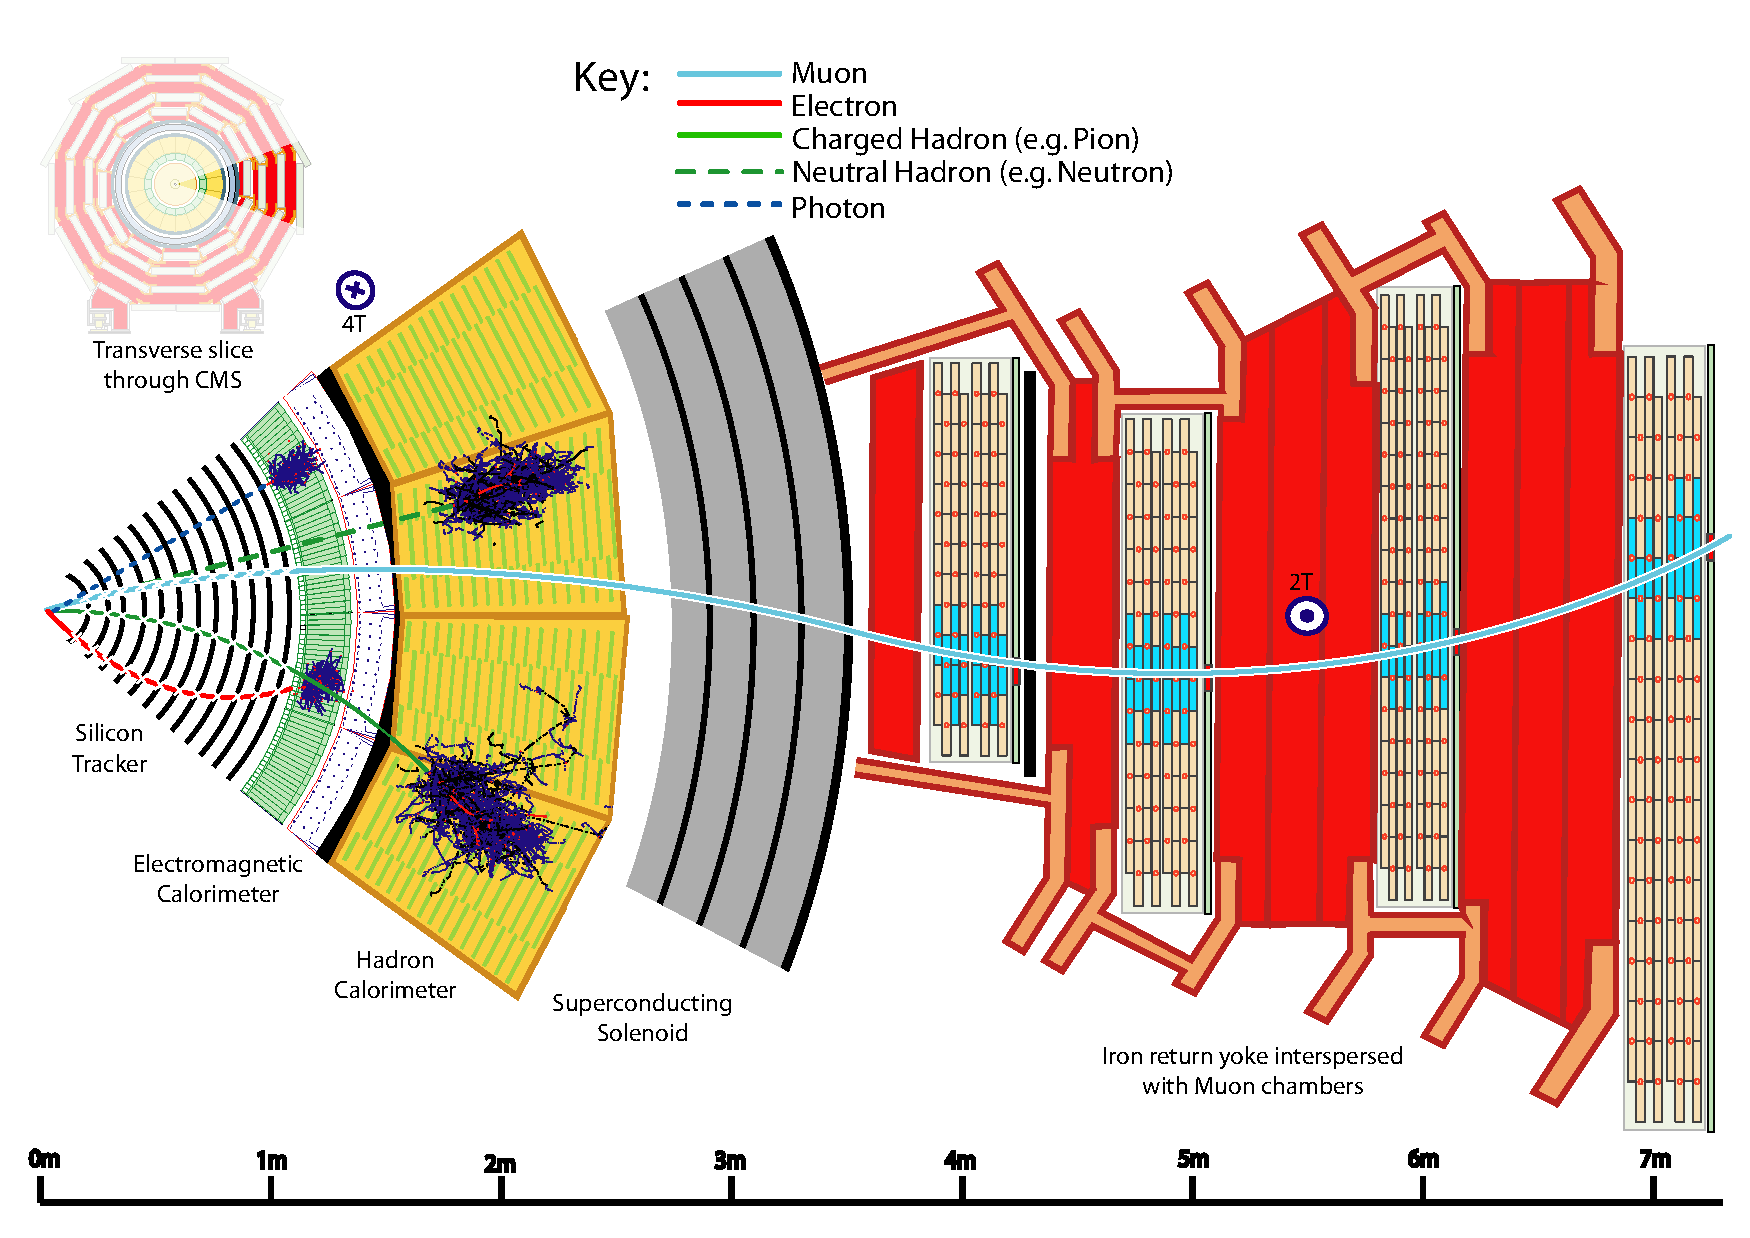
\includegraphics[width=0.7\linewidth]{figures/cms_slice_white}
  \caption[Transverse slice through the CMS detector]{Transverse slice
    through the CMS detector.  Particle traces are depicted to
  illustrate the function of the components~\cite{cmsoutreach}.}
  \label{fig:cms-slice}
\end{figure}

CMS is a general-purpose detector, designed to characterize a wide range of
proton-proton scattering events. Consequently, the design had to be hermetic, in
order to record the energy, charge, and momentum of as many scattering products
as possible. The detector is made up of a cylindrical barrel and two endcaps
with its longitudinal axis along the beamline.

Events produce a variety of final state particles that participate in different
sets of fundamental interactions. For this reason, CMS is composed of multiple
subdetectors, each optimized for measurements of specific sets of particles. A
central feature of CMS is its solenoid magnet, which produces a strong and
roughly constant magnetic field around the IP. Charged particles moving in a
magnetic field will follow a curved path with a radius that is proportional to
the momentum. A \textit{tracker} detects the ionization left by the passage of a
charged particle. If at least three points along the particle's path can be
determined, it is possible to reconstruct the radius of its trajectory and
calculate its momentum to charge ratio. Since leptons and stable hadrons have
integer units of elementary charge, particle momentum and the sign of its
assumed unit of charge (reflected in the sign of the track curvature) can be
reconstructed in practice.

A tracker alone is not sufficient to fully characterize events: neutral
particles will pass through undetected, and particles with different masses can
have the same momentum. To fully characterize a particle, only one unknown is
permitted in the equation $E^2 = p^2 + m^2$. For these reasons, CMS includes
\textit{calorimeters} that measure particle energy. Because the calorimeters
stop particles, the tracker must be the innermost detector; conversely, energy
loss in the tracker must be minimized to allow particle energy to be measured
accurately in the calorimeter.

Charged particles moving through matter are accelerated in the coulomb field of
atomic nuclei and emit bremsstrahlung radiation. Power loss for muons is
suppressed compared with electrons because of their higher mass, and as a
result, muons are not easily stopped in the calorimeters. A dedicated muon
tracking system is placed outside the calorimeters. Because other particles are
stopped in the calorimeters, a sign-of-charge (sign of track curvature) and
momentum measurement (radius of track curvature) are sufficient to fully specify
muons. One final type of particle, the neutrino, only interacts weakly and thus
is invisible to both trackers and calorimeters. By making the detector as
hermetic as possible, the presence of neutrinos or exotic neutral particles can
be inferred using conservation of momentum (see~\cref{sec:coordinates}).

The following sections describe the CMS components in more detail and are based
on~\cite{1748-0221-3-08-S08004}.

\subsection{Coordinate system and conventions}
\label{sec:coordinates}
The standard CMS coordinate system is used throughout this work, in which the
origin is defined as the nominal interaction point. The x-axis points towards
the center of the LHC ring, the y-axis points upwards towards the sky, and the
z-axis points along the beamline such that the system is right-handed.
Alternatively, polar coordinates are defined such that the distance from the
beamline in the plane perpendicular to the z-axis is called $r$. The azimuthal
angle $\phi$ is defined such that $\phi=0$ points along the x-axis. The polar
angle is defined such that $\theta=0$ points along the z-axis.

Conservation of momentum requires that the total outgoing particle momenta
equals the total incoming parton momenta. Because the momentum vector of the
incoming protons is entirely along the beamline, the momentum in the plane
transverse to the beamline must sum to zero, while the longitudinal component
depends on the unknown fraction of the total proton momentum that each parton
carried. Thus, longitudinal boosts vary from event to event in a distribution
that depends on the parton distribution functions (PDFs). For this reason, we
are usually only concerned with the transverse component of momentum \pT, from
which the transverse energy $E_T$ is defined for a particle of mass $m$:
\begin{align}
  \pT &= |\vec{p}| \sin\left(\theta\right) = \sqrt{p_x^2 + p_y^2}, \\
  E_T &= \sqrt{m^2 + \pT^2}.
\end{align}
Any deviation of the total transverse momentum from zero must have been carried
away by weakly interacting particles such as neutrinos. This quantity is called
the \textit{missing transverse momentum}: $\pTmiss = \abs{- \sum_i
\vec{p}_{T,i}}$, where the sum is over $i$ visible particles.
\todo[inline]{spacing is messed up in math mode}

The rapidity $y$ and the pseudorapidity $\eta$ are defined in terms of $\theta$:
\begin{align}
  y &= \frac{1}{2}\ln\left(\frac{E+p_z}{E-p_z}\right) \\
  \eta &= \frac{1}{2}\ln\left(\frac{|\vec{p}|+p_z}{|\vec{p}|-p_z}\right) = -\ln\tan\frac{\theta}{2}.\label{eq:eta}
\end{align}
The rapidity has the desirable feature that differences in rapidity are
invariant under boosts along the beam axis. Characterizing angles between
outgoing particles in terms of such a quantity allows for more convenient
comparison of events with different boosts. In other words, a histogram showing
the rapidity separation between two particles is meaningful despite being
populated by events whose center-of-mass frames have arbitrary longitudinal
boosts. The rapidity depends on both energy and momentum, which is difficult to
measure at high rapidities for highly relativistic particles. For this reason,
it is more common to work with the pseudorapidity, which is approximately equal
to the rapidity in the limit $|\vec{p}| \gg m$ because $E^2 = \abs{\vec{p}}^2 +
m^2 \implies E \approx |\vec{p}|$. It follows from~\cref{eq:eta} that $\eta=0$
corresponds to the vector perpendicular to the beamline, and $\eta=\infty$
($\eta=-\infty$) corresponds to a vector that is parallel (anti-parallel) to the
beamline. As $\eta$ gets closer to the beamline, equally spaced angular
separations represent larger and larger changes in $\eta$. This reflects the
intuitive fact that due to events being randomly boosted in the forward
directions (along the beamline), the average flux of particles is much higher in
the forward directions (at angles close to the beamline).

The angular separation in $\operatorname{\phi-\eta}$ space that describes solid
angles is called $\Delta R$, and it is also approximately Lorentz invariant.
$\Delta R$ is defined as
\begin{equation}
  \Delta R = \sqrt{\Delta\eta^2 + \Delta\phi^2}.
\end{equation}

\subsection{Solenoidal magnet}
The CMS magnet is a solenoid \SI{6}{\meter} in diameter and \SI{12.5}{\meter} in
length, capable of producing a highly uniform magnetic field in its inner bore.
It is large enough to accommodate the tracker and calorimeters, in order to
minimize energy losses when traversing the magnet, which would interfere with
their measurements. The standard operating field of \SI{3.8}{\tesla} requires a
current of~\SI{18160}{\ampere}, corresponding to a stored energy of
\SI{2.3}{\giga\joule}, which circulates in four layers of superconducting
niobium-titanium windings. A \SI{10000}{\tonne} steel return yoke, composed of
five barrel wheels and six endcap disks, guides the lines of magnetic field
around the outside of the solenoid and back into the other end. The return yoke,
because of its ferromagnetism and high magnetic permeability, becomes magnetized
by the field and thus passively adds to the field strength, focusing the field
in the region outside the solenoid where the muon system is located.

Charged particles moving inside the solenoid are deflected by the Lorentz force,
$\vec{F} = q(\vec{v} \times \vec{B})$. This force causes the component of the
particle velocity that is perpendicular\footnote{At CMS, the magnetic field
points along the z axis, so the component perpendicular to it is the transverse
component described in~\cref{sec:coordinates}.} to the magnetic field $v_T$ to
produce circular motion while the component of velocity parallel to the magnetic
field is unaffected, which results in a helical trajectory. Particle momentum
and charge can be determined from the radius and direction of curvature of the
particle's trajectory.

The windings of the solenoid are superconducting, which requires the magnet to
be cooled with liquid helium. One component in the cryogenic system is the cold
box, which contains the liquid helium heat exchangers. Run 1 went mainly
smoothly for the CMS magnet. Unfortunately, the cold box became contaminated by
oil in some components early in Run 2, causing erratic performance. As a result
only about \SI{75}{\percent} of 2015 proton-proton collision data were taken at
full magnetic field strength. During the year-end technical stop the affected
components were thoroughly cleaned and the oil recovery system was upgraded.
Magnet operation has subsequently run smoothly.

\subsection{Inner tracker}
\begin{figure}[htb]
  \includegraphics[width=\textwidth]{figures/tracker}
  \caption[Longitudinal cross section of the CMS inner tracker]{Longitudinal cross section of the CMS inner tracker~\cite{Chatrchyan:2014fea}.}
  \label{fig:tracker}
\end{figure}
The CMS inner tracker~\cite{tracker1,tracker2} (pictured in~\cref{fig:tracker})
is a cylindrical subdetector that is closest to the IP, consisting of an inner
silicon pixel detector and an outer silicon strip detector. It is designed to
measure the location and time that an electrically charged particle passes (a
\textit{hit}) while inducing minimal energy loss. Minimizing energy loss
requires the tracker to be capable of taking such accurate hit measurements that
the particle trajectory (or \textit{track}) can be reconstructed with just a few
hits. Being the innermost subdetector, it receives the highest flux of particles
and therefore radiation hardness is very important. The inner tracker covers
$|\eta|<2.5$ and has about \SI{200}{\meter^2} of active silicon area, which is
approximately the size of a tennis court. In the central region, the inner
tracker has a typical momentum resolution of \SI{0.7}{\percent} at \SI{1}{GeV}
and \SI{5.0}{\percent} at \SI{1000}{GeV}~\cite{Khachatryan:2010pw} and typical
impact-resolution for high momentum tracks of \SI{10}{\micro\meter}.
Unfortunately, the material making up the tracker corresponds to up to 0.5
interaction lengths at some pseudorapidities, which means that in the worst case
up to an \SI{85}{\percent} chance exists for a photon to convert or an electron
to emit bremsstrahlung radiation, and hadrons have a \SI{20}{\percent}
probability of a nuclear reaction before entering the
calorimeters~\cite{Sirunyan:2017ulk}. These interactions complicate event
reconstruction.

Silicon detectors are semiconductors, with electrical properties that are
determined by introducing small amounts of impurities that add mobile charge
carriers. N-type silicon has electron charge carriers, while p-type silicon has
lattice positions from which an electron is missing, resulting in mobile
\emph{holes}. The detector contains a junction between n-type and p-type
regions. An externally applied voltage provides a positive charge to the n-type
region, drawing electrons away from the junction, while a negative charge
applied to the p-type region draws away holes. This produces a region with no
mobile charge carriers near the junction, called the depletion zone, and no
current flows. The detector is a diode under reverse bias.

When a charged particle passes through the detector, it ionizes silicon atoms
near the junction, producing free electrons and holes. The electrons move to the
positive terminal and the holes to the negative terminal, generating a small
electric current that is amplified and recorded.

The tracker is subject to accumulated radiation damage, which creates extraneous
electron acceptor sites, depleting the n-type silicon and increasing the bias
voltage needed to maintain the maintain the depletion zone. This increases the
\textit{leakage current} that flows through the junction even when no ionization
is present~\cite{ma1989ionizing} and can cause breakdown of the junction and
\textit{thermal runaway}. To reduce the rate of radiation damage, the tracker is
cooled to \SI{-10}{\celsius}.

\subsubsection{Pixel detector}
The detector closest to the IP requires the highest spatial resolution. Referred
to as the \textit{pixel detector}, it contains millions of very small detector
elements called pixels, each $\SI{100}{\micro\meter} \times
\SI{150}{\micro\meter}$ in area and $\SI{320}{\micro\meter}$ in thickness. The
high-luminosity LHC environment produces an effective p-doping over time, which
requires a continually increasing bias voltage. For this reason, high dose
n-implants are introduced onto an n-type substrate with p-type rings to isolate
individual pixels and p-type silicon on the back side, which allows the sensor
to operate while partially depleted. Because of the presence of electric and
magnetic fields, the direction that the liberated electron-hole pairs drift is
affected by the Lorentz force, leading to sharing of charge between neighboring
pixels. This effect is exploited to improve the pixel resolution. During Run 1,
the pixel detector had three concentric cylindrical barrel pixel layers (BPix)
at radial distances between \SIrange{4.4}{10.2}{\centi\meter} from the IP, and
two pixel layers (FPix) in each of the two endcaps which extend out to roughly
$z=\pm\SI{50}{cm}$. Partially into Run 2 during the year-end technical shutdown
in 2016, the pixel detector was upgraded~\cite{1748-0221-12-02-C02033} to have
four barrel layers and three endcap layers, in addition to faster readout chips
and an improved cooling system. The upgrade resulted in an increase from
\num{66} million total pixels to 124 million.

\subsubsection{Silicon strip tracker}
The pixel detector is surrounded by the silicon strip tracker (SST), which fills
a volume between \SIrange{20}{116}{\centi\meter} radially and out to
\SI{118}{\centi\meter} in $z$, covering $|\eta| \leq 2.5$. Because the particle
flux at this distance is smaller compared with the pixel region, a lower
granularity design is sufficient. The SST has approximately \num{9.3} million
strips composed of p-type implants on an n-type substrate with a solid n-type
back. The strip system is divided into one barrel and two endcap regions. The
barrel consists of the tracker inner barrel (TIB, four layers) and the tracker
outer barrel (TOB, six layers). Each endcap consists of a tracker endcap (TEC,
nine layers of disks, each with up to seven rings of radial-strip detectors) and
a tracker inner disk (TID, nine layers). Similar to the pixel detector, charged
particles liberate conduction-band electrons which drift towards readout
sensors. The strip detectors are inclined with respect to the z-axis to be
approximately perpendicular to the paths of particles radiating from the IP.

\subsection{Calorimeters}
Calorimeters measure the energy of particles by absorbing them; in other words,
they induce particle showers within their volume, which dissipate kinetic
energy. The active material of a calorimeter is a dense medium. Incident
particles interact with the medium through electromagnetic or strong processes
and produce secondary particles. These secondary particles also interact,
generating a subsequent shower of particles with progressively smaller energies,
which deposit energy that is proportional to the energy of the incident
particle.

CMS has two calorimeters. The electromagnetic calorimeter (ECAL)  absorbs mainly
photons and electrons. Charged hadrons also deposit energy, but may not be
absorbed. The hadronic calorimeter (HCAL) measures the energy of hadrons.

\subsubsection{Electromagnetic calorimeter}
\begin{figure}[htb]
  \centering
  \includegraphics[width=0.8\textwidth]{figures/ecal}
  \caption[Layout of the CMS electromagnetic calorimeter]{Layout of the CMS electromagnetic calorimeter~\cite{1748-0221-3-08-S08004}.}
  \label{fig:ecal}
\end{figure}
Surrounding the tracker, the ECAL (shown in~\cref{fig:ecal}) is composed of
transparent lead-tungstate scintillator crystals. Lead-tungstate was chosen
because of its radiation hardness, fast light output (\SI{80}{\percent} in
\SI{25}{\nano\second}), short radiation length (the mean distance an incoming
electron traverses before losing all but $1/\Pe$ of its energy) of
\SI{0.89}{\centi\meter}, and a small Moli\`er radius (the radius of a cylinder
containing \SI{90}{\percent} of the shower energy) of \SI{2.2}{\centi\meter}. A
short radiation length and small Moli\`er radius is desirable in order to fully
absorb incoming particles with a compact design. The electromagnetic shower
induced in the crystals causes the energized scintillator atoms to emit light in
proportion to the size of the shower. This scintillation light is collected by
avalanche photodiodes in the barrel and photomultiplier devices called vacuum
phototriodes in the endcaps. There are \num{61000} crystals in the ECAL barrel
region, which covers $|\eta| < 1.479$, and \num{7324} crystals in each of the
ECAL endcaps, covering $1.479 < |\eta| < 3$. The crystals vary
between~\SIrange{22}{23}{\centi\meter} in length.

A finer-grained detector, the ECAL preshower (ES), is placed in front of each
endcap. It has a total thickness of about \SI{20}{\centi\meter} and uses a
sampling design consisting of two layers of lead radiators to induce showers,
interleaved with two layers of silicon strip sensors to measure the deposited
energy. The intended function of the ES was to help distinguish $\pi^0
\rightarrow \gamma\gamma$ decays from single high-energy prompt photons.
Unfortunately, the large number of neutral pions produced through hadronic
interactions with the tracker material in practice degrades the ES capabilities
and thus the energy deposits in the ES are simply added to corresponding
deposits in the ECAL.

Over time, radiation induces lattice damage in the lead tungstate crystals and
reduces their transparency. Consequently, a calibration system is necessary.
This system uses the LHC abort gaps to measure the baseline electronic noise
(\textit{pedestal}) levels and fire laser or LED pulses into the crystals to
measure their transparency at regular intervals during data collection (on the
order of once per hour).

\subsubsection{Hadronic calorimeter}
The HCAL is a sampling calorimeter composed of interleaved layers of brass
absorber and tiles of plastic scintillator material. Brass is an ideal material
for this purpose because it is non-magnetic and has a relatively short
interaction length (\SI{16.4}{\centi\meter}), which is the average distance a
particle will travel before interacting with the absorber. The HCAL surrounds
the ECAL, and extends radially between \SIrange{1.77}{2.95}{\meter} from the
beamline, providing a minimum of six interaction lengths for hadrons passing
through it.

Incident hadrons cause showers of hadrons and leptons in the brass, which causes
light to be produced in the scintillating layers in proportion to the amount of
energy deposited. The light from the tiles is collected by wavelength-shifting
fibers that are grouped into readout towers before being transmitted to hybrid
photodiodes for amplification and readout.

The HCAL barrel (HB) region covers $|\eta| < 1.3$, and there are two HCAL end
caps (EC), with each covering $1.3 < |\eta| < 3$. The EC and HB sections do not
fully absorb all hadronic showers; any components passing beyond the HCAL are
referred to as \textit{hadronic punchthrough}. To measure shower energy
deposited outside the HB, there is an extra layer of scintillator tiles located
outside the solenoid, concentric to the HB, called the HCAL outer, or tail
catcher. This outer layer uses the solenoid coil itself as an absorber. At
either end of CMS, there are additional sections called the HCAL forward (HF)
that covers $4.5 < \abs{\eta} < 5.2$ and absorbs particles emerging from the IP
at shallow angles. The HF absorbs the majority of the energy from the collision
and so is made of steel absorber plates interleaved with layers of quartz
fibers; interactions in the absorber produce showers of particles that pass
through the quartz fibers, generating flashes of Cerenkov light.

\subsection{Muon subsystem}
\begin{figure}[htb]
  % \centering
  \includegraphics[width=\textwidth]{figures/muon_quadrant}
  \caption[Cross section of one quadrant of the CMS muon system]{An $R-Z$ cross section of one quadrant of the CMS muon system~\cite{cms-tdr-1}.}
  \label{fig:muonquadrant}
\end{figure}
Muons lose less energy due to bremsstrahlung than electrons because of their
higher mass and do not interact via the strong force. Consequently the CMS muon
subsystem~\cite{muonTDR} is the outermost detector since muons are the only
charged particle that makes it that far. Since the mass of the particle is
known, it is only necessary to measure its charge and momentum.

The muon tracker (MT) subsystem consists of a cylindrical barrel region and two
endcaps. The barrel is divided along the beam axis into five separate wheels
with four concentric layers, alternating with layers of the return yoke.
Throughout Run 1, the endcaps had three disks (\textit{stations}) each; during
LS1 a fourth disk was installed~\cite{Guiducci:1966038}.

Because it is so far from the IP, the MT must cover a much greater area than the
inner trackers to be hermetic. Consequently it must be less expensive per unit
area to be practical; however, it does not require as high a resolution as the
inner detectors. Gas ionization chambers of three types were selected.

Drift tubes (DTs) are used in the barrel region because it has lower muon rates.
There are four layers of stations covering $\abs{\eta} < 1.2$. The DTs consist
of $\SI{13}{\mm} \times \SI{42}{\mm} \times \SI{2.4}{\meter}$ cells filled with
a mixture of carbon dioxide and argon gas. An anode wire held at a positive
potential of \SI{3.6}{\kilo\volt} runs the length of the tube, while electrode
strips on the \SI{42}{\mm} walls are held at \SI{1.8}{\kilo\volt} and on the
\SI{13}{\mm} walls are held at \SI{-1.2}{\kilo\volt}. A muon passing through the
tube ionizes the gas, producing free electrons and positively charged ions that
drift to the wire or strips, creating a signal that is amplified and measured.
Groups of four cells are stacked, staggered by half a cell to eliminate dead
spots, to form a superlayer (SL). The DTs are arranged in four concentric
cylinders around the beam axis, called stations, which alternate with layers of
the steel plates that form the magnet return yoke. The three inner stations have
three SLs each; two have wires running parallel to the beamline in order to
measure $r-\phi$ and one has wires perpendicular to the beamline in order to
measure $\eta$. The outer station has two SLs with wires that are parallel to
the beam and only measure $r-\phi$.

Cathode strip chambers (CSCs) with higher resolution than the drift tubes are
used in the endcaps, where the magnetic field is nonuniform and the muon rates
are higher. Each endcap has four disks of CSCs covering $1.2 < \abs{\eta} <
2.4$. As with the barrel, the disks alternate with steel plates of the return
yoke. Each CSC is trapezoidal in shape with seven layers of cathode panels that
have strips at constant $\phi$ intervals pointing radially out from the beam.
These are interleaved with six panels of anode wires, oriented roughly
perpendicularly to the cathode strips, to measure the radial position of the
hit. Between the panels is a mixture of carbon dioxide, argon, and carbon
tetrafluoride. CSCs use a mechanism similar to the DTs. An electrostatic
potential is maintained between the anodes and cathodes; incoming muons ionize
gas molecules, producing ions that drift towards the wire or strips, creating a
small current pulse that is amplified and recorded.

Resistive plate chambers (RPCs) are gaseous parallel-plate detectors. The
mechanism of operation is similar to the CSCs, except that there is a very
narrow gap of \SI{2}{\milli\meter} between the charged plates. This gap means
they have a lower spatial resolution, but a very fast response time of only one
nanosecond. Because the CSCs and DTs alone are not fast enough to unambiguously
associate muons with a specific bunch crossing, RPCs are used throughout the
system, covering the entire range of pseudorapidity.

The spatial resolution achieved per chamber is \SIrange{80}{120}{\micro\meter}
in the DTs, \SIrange{40}{150}{\micro\meter} in the CSCs, and
\SIrange{8}{12}{\milli\meter} in the RPCs. The efficiency for reconstructing
hits and track segments in the muon system is in the range
\SIrange{95}{98}{\percent}~\cite{Chatrchyan:2013sba}.

\subsection{Trigger and data acquisition}
Each crossing between two bunches of protons at the IP in which protons collide
is called an \textit{event}. During Run 1, the LHC normally provided $pp$
collisions with a bunch spacing of \SI{50}{\nano\second}. In Run 2, the bunch
spacing was reduced to \SI{25}{\nano\second}. This corresponds to a peak (in
other words, excluding abort gaps) crossing frequency of \SI{20}{\mega\Hz} and
\SI{40}{\mega\Hz} for Run 1 and Run 2, respectively. The raw information read
out by the detector for each event is $\mathcal{O}(\SI{500}{kB})$, meaning that
CMS produces tens of terabytes of data per second, far exceeding the pace at
which the data can be recorded. This rate necessitates a \textit{trigger} system
that quickly selects the most interesting events for storage. Discarded data
cannot be recovered, so a properly functioning trigger system is critical to the
success of the experiment. Periods during which events are not recorded because
systems are busy processing existing data are referred to as \emph{dead time}
and should be minimized. The event rate is reduced in two stages: first, a
faster, hardware-based Level 1 (L1) trigger reduces the event rate to
\SIrange{80}{100}{\kilo\hertz}. Next, a slower, software-based High Level
Trigger (HLT) further reduces the event rate to approximately
\SI{1}{\kilo\hertz}.

The time between the collision and when the L1 delivers a final decision is
referred to as the \emph{latency}. During this time, all of the data from the
detector are buffered in a pipeline before being either discarded or forwarded
on to the HLT. The L1 latency is \SI{4}{\micro\sec}, which coincides with the
length of the LHC abort gap, making it possible to operate with zero dead time.
This goal is accomplished with fast electronics (field programmable gate arrays)
that construct local \emph{trigger primitives} from the raw output of the
calorimeters and muon systems (track reconstruction is too computationally
expensive to complete on the L1 timescale). The calorimeter output channels are
grouped into trigger towers. Trigger primitive generators calculate $E_T$ sums
for each tower and send them to the Regional Calorimeter Trigger, which combines
these values with quality information about the shower pattern to identify
candidate electrons and photons, along with $E_T$ sums for groups of $4 \times
4$ towers. These quantities are then passed to the Global Calorimeter Trigger
(GCT), which calculates the sum $E_T$, \pTmiss and the scalar sum of transverse
energy $H_T$. Track segments and hit patterns from the DT and CSC local triggers
are sent in parallel to their respective track finders, which sort the trigger
primitives by \pT and quality. Information is shared between the two track
finders so that overlapping track segments can be linked. The RPCs assemble muon
candidates from regional hit patterns and, because they are much faster than the
CSCs and DTs, provide unambiguous bunch crossing identification. The best
candidates from all three systems are passed on to the Global Muon Trigger
(GMT), which combines the information for improved momentum resolution and
efficiency.

The highest-quality objects (i.e., electrons/photons, muons, jets, or \Ptau
leptons) from the GCT and GMT are forwarded to the Global Trigger (GT). A
\textit{path} is a set of algorithms and requirements on objects in an event. L1
paths have simple criteria; for example, the event must contain at least one
muon exceeding a given threshold, or the event must contain combinations of
several objects. A trigger menu with a maximum of 128 different paths could be
specified during Run 1. During LS1, the L1 trigger was
upgraded~\cite{Tapper:1556311}, which added several L1 improvements, including
adding fast pileup subtraction and expanded the menu size to a maximum of 256
paths.

If an event satisfies the criteria of any path in the L1 menu, the GT sends an
L1 Accept signal to the Timing, Trigger, and Control (TTC) system which controls
readout of the subdetector frontend buffers to the front-end drivers (FEDs). FED
fragments are subsequently merged by the Event Builder and passed to the HLT.
The HLT is a version of the sophisticated event reconstruction software used in
offline analysis and achieves similar quality reconstruction. The HLT had a per
event time budget of \SI{175}{\sec} during 2012. This longer timescale is made
possible by a computer cluster with \num{13000} cores which can process multiple
events simultaneously. The HLT menu is composed of more than \num{400} paths.
HLT paths are more complex than at L1, consisting of a sequence of
reconstruction and filtering steps. Products are filtered as algorithms are run.
In this way, selections relying on calorimeter and muon system data, which are
run first, reduce the number of events over which the computationally expensive
tracker reconstruction is performed.

More details on the trigger system can be found
in~\cite{1748-0221-12-01-P01020}.


\chapter{Object reconstruction and selection}
\label{chap:objects}
The CMS subdetectors produce raw electrical signals, from which \emph{physics
objects} are inferred as software representations of particle observables. This
process is called \emph{reconstruction} and is described
in~\cref{sec:particle-flow}. In~\cref{sec:object-selection}, the selection
criteria for physics objects used in this work are discussed. Except where
noted, features are common to both the \eightTeV measurement (presented
in~\cref{chap:8-TeV}) and the \thirteenTeV measurement (presented
in~\cref{chap:13-TeV}).

\section{Particle flow}
\label{sec:particle-flow}
CMS uses a reconstruction approach called \emph{Particle Flow} (PF), which takes
advantage of information provided by each of the CMS subdetectors, as well as
the correlations between these observations to construct a global picture of
each event. The following description of the CMS PF algorithms is based on
reference~\cite{Sirunyan:2017ulk}.

The reconstructed origin of a set of physics objects is called a \emph{vertex}.
An example of a vertex is the origin of the physics objects emerging from a
proton-proton collision. As shown in~\cref{fig:luminosity}, each bunch crossing
results in multiple proton-proton collisions. The majority of these are pileup.
The vertex for which $\sum\pT^2$ is highest is most likely to be associated with
the production of heavy particles, and is chosen to be the \emph{primary vertex}
(PV). For the \eightTeV analysis, the sum is taken over all charged particles
that were used in the vertex reconstruction. For the \thirteenTeV analysis, the
sum is taken over all charged leptons and jets formed from charged tracks used
in the vertex reconstruction, in addition to the \pTmiss, which is computed as
the magnitude vector sum of \pT from all PF candidates.

An iterative approach is used~\cite{Chatrchyan:2014fea} to reconstruct particle
trajectories in the inner tracker. Each iteration begins with seeds generated
from a few tracker hits. Next, trajectories are built by adding hits from
successive track layers. Finally, track-fitting using a Kalman
filter~\cite{Fruhwirth:1987fm} is performed to calculate the track origin and
direction, and the \pT. In each iteration, tracks are subject to quality
requirements on the seeds, $\chi^2$ fit, vertex compatibility, \pT, $|\eta|$,
and number of hits. After each iteration, hits that have been assigned to tracks
are removed from the available hit pool. The first iteration applies stringent
criteria, which produces a low rate of misreconstructed tracks with moderate
tracking efficiency. Over 10 total iterations, the criteria are progressively
relaxed as the algorithms become more complex and time-consuming. After the size
of the hit pool has been sufficiently reduced, later iterations can perform more
computationally intensive searches for displaced tracks with secondary vertices
outside the interaction region (mainly due to photon conversions or nuclear
interactions in the tracker material, b jets, $\Delta$ decays, \etc)

Most electrons radiate bremsstrahlung photons due to the coulomb field of atomic
nuclei as they pass through the tracker. These photons are emitted in a
characteristic arc due to the azimuthal bending of the electron track in the
magnetic field. To account for these interactions, tracks likely to be electrons
are selected after the iterative procedure described above based on their number
of hits and $\chi^2$ fit. The track-fitting is then repeated with a Gaussian Sum
Filter (GSF)~\cite{0954-3899-31-9-N01}, which approximates the electron energy
loss as a sum of Gaussian distributions instead of a single Gaussian, resulting
in an improved momentum resolution.

The determination of particle energy measured in the calorimeters is
accomplished with a \emph{clustering} algorithm, which takes as input a map of
individual energy deposits and outputs groupings of energy deposits that can be
associated with candidate physics objects. First, \emph{cluster seeds} are
determined by identifying calorimeter cells with energies exceeding a predefined
threshold. Next, clusters are built up by adding adjacent cells with energy
deposits exceeding typical electronic noise levels.

After the PF elements have been assembled, a \emph{linking} algorithm evaluates
the degree of the compatibility between different subdetector elements that are
nearest neighbors in the $(\phi, \eta)$ plane to determine which are likely to
be associated with the same particle. Tracks are extrapolated from the last hit
measured in the tracker to the PS and subsequently to the ECAL and HCAL. If the
extrapolation falls within the cluster boundaries, a link is established. ECAL
clusters that are consistent with the extrapolation of tangents from points in
which inner tracks intersect with tracker layers are linked as possible
bremsstrahlung photons. Photons have a substantial probability to pair produce
in the tracker material, so a similar process is used to identify possible
photon conversions. If the $(\phi, \eta)$ cluster position in the ECAL is within
the cluster envelope in the HCAL, a link is established. \emph{Global muons} are
formed if tracks in the inner tracker and tracks in the muon system can be
linked by interpolating towards each other with an acceptable $\chi^2$.
\emph{Tracker muons} are formed if the extrapolation out to the muon track from
the inner track is sufficiently consistent. The highest-quality links are used
to form sets of PF elements that are linked, or have common elements that are
linked. These sets are called \emph{blocks}.

Following linking, PF elements are assigned particle identifications. To reduce
combinatorics, elements are removed from blocks after assignment. Muons are
assigned first because of the high purity with which they can be reconstructed,
and they are required to satisfy any of three sets of criteria. Particle
\emph{isolation} quantifies the degree to which a particle is separated from
others. Isolated muons are identified if the sum of the track \pT and transverse
energy of calorimeter deposits in a cone with $R=0.3$ does not exceed
\SI{10}{\percent} of the muon \pT. Nonisolated muons are identified if they pass
a more stringent selection~\cite{Chatrchyan:2013sba} optimized for muons within
jets. Finally, muons that fail the tight selection because of problems with the
inner track reconstruction, but which have a sufficiently high-quality fit in
the muon system, are assigned as PF muons and removed from their blocks.

Because of the tendency for electrons to emit bremsstrahlung photons, and for
photons to pair produce electrons in the tracker material, electrons and
isolated photons are reconstructed together, following muon reconstruction.
Electron candidates are seeded with tracks in the inner tracker linked to
sufficiently large energy deposits in the ECAL. Photon candidates are seeded
from similar energy deposits that have no linked corresponding inner tracks.
Electron and photon candidates must meet requirements on the distribution of
energy deposits in the calorimeters. Photons additionally must be isolated from
other tracks and energy deposits. A multivariate discriminator based on track
variables and energy distribution patterns is used to select electrons.

% http://ific.uv.es/tical/Publications/InternalNotes/Nota_Atlfast.pdf
After muons, electrons, and isolated photons have been classified and removed
from their blocks, hadrons and nonisolated photons are identified. The majority
of jet energy is carried by charged hadrons, then photons, and finally neutral
hadrons. For this reason, within the tracker acceptance, ECAL clusters that are
not linked to inner tracks are classified as photons, and HCAL clusters that are
not linked to inner tracks are classified as neutral hadrons. If the calorimeter
clusters are linked to tracks, each track is assumed to give rise to a charged
hadron. If the calibrated calorimeter energy is greater than the total track
momenta by more than what is expected from the energy resolution to measure
charged hadrons, the surplus is assumed to be carried by photons and neutral
hadrons: up to the ECAL energy, the surplus is assigned as a photon, and any
energy above that is assigned as a neutral hadron. Outside of the tracker
acceptance, where charged and neutral hadrons cannot be distinguished, ECAL
clusters with no associated HCAL cluster are classified as photons, while ECAL
clusters that are linked to HCAL clusters are classified as arising from the
same hadronic shower. The response produced in the ECAL to photons and charged
hadrons with equivalent energy is different and must be corrected for after
particle identification has been made.

The anti-$k_t$ algorithm~\cite{1126-6708-2008-04-063} is used to identify which
PF candidate hadrons belong to the same jet. The quantity
\begin{eqnarray}
  d_{ij} = \frac{\Delta_{ij}^2}{R^2 \max(k_{ti}, k_{tj})}
\end{eqnarray}
is calculated for all possible candidate pairs $i,j$, where $R$ is a
characteristic radius parameter, $\Delta_{ij}^2 = (y_i - y_j)^2 +
(\phi_i-\phi_j)^2$, and $k_{ti}$, $y_i$, and $\phi_i$ are respectively the
transverse momentum, rapidity, and $\phi$-coordinate of candidate $i$. The pair
that minimizes $d_{ij}$ is replaced by a clustered candidate with the sum of
their four-momenta. If all possible $d_{ij} > 1/k_{ti}$ for any candidate, it is
promoted to a jet and removed from consideration. The process is repeated until
no candidates remain. If there are many soft particles and only one hard
particle within a radius $2R$, the minimum $d_{ij}$ will be dominated by the
momentum of the "seed" hard particle, which will accumulate soft particles,
resulting in a jet that is a circle around the hard particle in the $\phi-\eta$
plane of radius R. If there are two hard particles that are more than $R$ apart
but less than $2R$, there will be two jets, with more of the soft particles
naturally assigned to the higher-$k_t$ particle. If there are two hard particles
less than $R$ apart, they will be merged into a single jet.

Anti-$k_t$ jets with $\text{R}=0.5$ are used in the \eightTeV analysis. Because
the average jet energy increases with increasing center-of-mass energy,
resulting in narrower jets, the cone size was reduced to $\text{R}=0.4$ in the
\thirteenTeV analysis.

Because top quarks almost always decay to b quarks, identifying jets from b
quarks (called \emph{b-tagging}) is critical for selecting \ttW and \ttZ events.
Because the b quark is the lighter of the third generation quark doublet, it
decays via a generation-changing process to c or u quarks, which are
off-diagonal CKM matrix elements and therefore suppressed. This results in a
substantially longer b quark lifetime than expected for their mass. On the other
hand, it is short enough that decays still occur inside the detector. The long
lifetime of b hadrons in jets originating from the hadronization of b quarks
allows them to travel $\mathcal{O}(\SI{1}{mm})$ before decaying at a displaced
\emph{secondary vertex}. In the \eightTeV analysis, a Combined Secondary Vertex
(CSV) b-tagging algorithm was used~\cite{1748-0221-8-04-P04013}. The CSV
algorithm uses variables related to the distance from a track's point of origin
to the PV (the impact parameter, or IP) along with secondary vertex information
to produce a continuous score between zero and one that is assigned to each jet.
Higher scores indicate that the jet is more likely to have originated from a b
quark than a light-flavor quark or gluon. In the \thirteenTeV analysis,
improvements were made to allow for the inclusion of additional variables,
improving the tagging efficiency by several percentage points, and is referred
to as CSVv2~\cite{CMS-PAS-BTV-15-001}.

\section{Object selection}
\label{sec:object-selection}
Our analyses, like most on CMS, rely on the PF and jet clustering procedure
described above. Additional requirements, optimized for selecting \ttW and \ttZ
events, are discussed below.

\subsection{Leptons}
\label{ssec:leptons}
For the \ttW and \ttZ measurements, differentiating \emph{prompt} from
\emph{nonprompt} leptons is critical. Prompt leptons are muons or electrons
arising either directly from a W or Z boson parent, or from a tau lepton which
arise directly from a W or Z boson parent. Prompt leptons that have
misidentified charge are called \emph{charge flip} leptons. Nonprompt leptons
arise mainly from b hadron decays, misidentified jets, or photon conversions.

Prompt leptons are generally more isolated from other objects in the event than
nonprompt leptons, which are often produced in hadronic decays. To assess the
degree of isolation, the scalar sum of PF particles within a cone of $\Delta R =
\sqrt{\smash[b]{(\Delta \eta)^2 + (\Delta \phi)^2}} = 0.4$ (or $\Delta R = 0.3$
for electrons in the \thirteenTeV analysis) around the lepton direction is
calculated. To account for the charged component of pileup, the sum \pT of
charged particles not originating from the PV is subtracted. To account for the
neutral component, half of the charged PU contribution is subtracted in the
\eightTeV analysis. In the \thirteenTeV analysis, a $\rho(\eta)$ correction is
used as described in~\cref{sec:jet-clustering}. The ratio of this corrected sum
to the lepton \pT is called the relative isolation. Prompt leptons are also
characterized by low minimum displacement of the track from the vertex in the
transverse ($d_{xy}$) and longitudinal ($d_z$) planes, and by the ratio of the
three-dimensional impact parameter to its uncertainty ($\text{SIP}_\text{3D}$).
Electrons are additionally required to pass cuts on the score from an ElectronID
MVA classifier which combines discriminating power from a set of shower-shape,
track-cluster consistency, and track quality variables. This classifier was
re-optimized for the \thirteenTeV analysis.

Analysis-specific criteria, along with a description of the different criteria
categories used for event selection and data-driven background estimations, are
summarized below for the \eightTeV and \thirteenTeV analyses.

\subsubsection{\eightTeV}
The \eightTeV analysis imposes requirements related to the properties of the
nearest jet. A nearby jet with a high CSV value indicates that the lepton is
likely to be nonprompt, originating from b-hadron decay. Furthermore, the ratio
of lepton \pT to that of the nearest jet tends to be lower for such leptons.

Four sets of lepton selection criteria are defined: preselected, loose, tight,
and good charge. Preselected leptons, with criteria designed to select both
prompt (selected with $\sim \SI{100}{\percent}$ efficiency) and nonprompt
leptons, are used in the data-driven background estimations described
in~\cref{sec:8-modeling}. Tight leptons, used to select events in the SS
dilepton and three lepton channels, must pass more stringent criteria designed
to accept prompt and reject nonprompt leptons. The efficiency for accepting
prompt leptons passing the tight criteria is \SIrange{68}{98}{\percent} for
muons and \SIrange{49}{93}{\percent} for electrons, while \SI{80}{\percent} of
nonprompt leptons are rejected. Loose leptons, selected with a less stringent
set of criteria, are used to select events in the OS dilepton and four lepton
channels, where there are fewer nonprompt leptons. These cuts accept
\SIrange{93}{99}{\percent} of prompt muons and \SIrange{89}{96}{\percent} of
prompt electrons while rejecting $\sim \SI{50}{\percent}$ of nonprompt leptons.
In addition to the preselected, loose, or tight criteria, additional charge ID
requirements are imposed to reject charge flip leptons. This charge ID cut has
\SI{99}{\percent} efficiency for right charge muons and rejects $\sim
\SI{100}{\percent}$ of charge flip muons; for electrons, the efficiency ranges
from \SIrange{85}{100}{\percent}, while more than \SI{97}{\percent} of charge
flip electrons are rejected. These four sets of selection criteria are
summarized in~\cref{tab:8-TeV-leptons}.
\begin{table}
  \centering
  \caption[Lepton Selection Criteria (\eightTeV)]{
    Lepton Selection Criteria (\eightTeV)
  }
  \input{tables/eight-TeV/leptons}
  \label{tab:8-TeV-leptons}
\end{table}

\begin{table}
  \input{tables/thirteen-TeV/leptons}
\end{table}

\subsubsection{\thirteenTeV}
\label{subsec:13_lep_selection}
The \thirteenTeV analysis defines two sets of lepton selection criteria. Loose
leptons are used in the data-driven background estimations. Tight leptons are
used to select signal events. Additional quality criteria are imposed,
corresponding to the medium working point recommended by the muon Physics Object
Group (POG). These selection criteria are summarized
in~\cref{tab:13-TeV-leptons}.
% muon POG MediumID2016 WP: http://cms.cern.ch/iCMS/jsp/db_notes/noteInfo.jsp?cmsnoteid=CMS%20AN-2017/045


\subsection{Jets and missing energy}
\label{sec:jet-clustering}
Jet energy corrections (JECs), described in detail in
reference~\cite{1748-0221-12-02-P02014}, are required to calibrate the
reconstructed jet energy to match the true parton energy. To mitigate the
effects of pileup, charged hadrons that do not originate from the PV are removed
before jet clustering as described in reference~\cite{CMS-PAS-JME-14-001}. To
account for neutral hadrons from pileup, the average energy density as a
function of the pseudorapidity $\rho(\eta)$ is calculated for each event and,
for each jet, multiplied by the effective jet area and subtracted. Jets coming
from pileup vertices are removed using a multivariate
discriminator~\cite{CMS-PAS-JME-13-005} based on tracking information and jet
shape, with sensitivity driven by the ratio of the total \pT from charged
candidates that do not originate from the PV to the total \pT of all charged
candidates in the jet and the average spread in \pT among jet PF candidates.
Additional corrections, parameterized in $\eta$ and jet \pT, are applied to
account for residual differences between data and simulation, and the nonlinear
detector response to hadrons. To reject fake jets from misreconstruction and
instrumental noise, jets must have at least two PF constituents and the fraction
of their energy from the ECAL or HCAL deposits must not exceed
\SI{99}{\percent}.

Jets with $|\eta| < 2.4$ and $\pT >$ \SI{25}{~GeV} ($\pT >$ \SI{30}{~GeV}) are
selected for the \eightTeV (\thirteenTeV) analysis. To prevent double counting,
jets must be separated from the selected leptons by $\Delta R > 0.5$  for the
\eightTeV analysis and $\Delta R > 0.4$ for the \thirteenTeV analysis.

Loose and medium working points for the b-tagging output discriminant are used,
defined to operate with a $\approx$\SI{10}{\percent} and
$\approx$\SI{1}{\percent} chance, respectively to incorrectly tag light quark or
gluon jets (i.e., to \emph{mistag}). This approach corresponds to an efficiency
of $\approx$\SI{85}{\percent} to correctly tag b jets for the loose working
point and $\approx$\SI{70}{\percent} for the medium working point, depending on
the jet \pT and $\eta$. To satisfy the loose or medium working point,
$\text{CSV} > 0.244$ and $\text{CSV} > 0.679$ were required respectively for the
\eightTeV analysis. For the \thirteenTeV analysis, this requirement corresponded
to $\text{CSVv2} > 0.5426$ and $\text{CSVv2} > 0.8484$.

The \pTmiss is defined as the magnitude of the sum of the negative transverse
momenta of all of the PF particles. Because pileup can contribute to \pTmiss,
the \eightTeV analysis makes use of the variable \HTmiss, computed as the sum of
the negative transverse momenta of selected jets and leptons. The \HTmiss is
more robust than \pTmiss at the expense of reduced resolution.


\chapter{Observation of top quark pairs produced in association with a vector boson in proton--proton collisions at $\sqrt{\text{s}} = \SI{8}{TeV}$}
\label{chap:8-TeV}

This chapter summarizes \ttW and \ttZ cross-section measurements that were
completed using \SI{8}{TeV} pp collision data corresponding to an integrated
luminosity of 5$5$\SI{19.5}{\per\femto\barn} collected during Run 1 of the LHC. The \ttZ
analysis was the first to exceed the $5\sigma$ significance threshold, which is
considered sufficient to constitute the discovery of a hypothesized process. The
reinterpretation of this measurement within the context of effective field
theory will be described in~\cref{chap:eft}.

More details on this analysis can be found in reference~\cite{brinkerhoff-thesis}.

\section{Event selection}
\label{section:8-event-selection}
\begin{table}
  \input{tables/eight-TeV/final_states}
\end{table}
We searched for \ttW and \ttZ events by optimizing selection criteria for each
of several possible decay channels. At least one of several triggers, all based
on lepton energies, had to be satisfied for data collection: either a dilepton
trigger ($\Pe\Pe$, $\Pe\mu$, $\mu\mu$) with \pT thresholds of 17 and \SI{8}{GeV}
or a trielectron trigger with thresholds of 15, 8, and \SI{5}{GeV}. To ensure
that events are recorded with the triggers operating near their maximum
efficiency, selected leptons must have $\pT > \SI{10}{GeV}$, with at least one
$\pT > \SI{20}{GeV}$. To reduce selection of $\Upsilon$ and J/$\psi$ events the
invariant mass of any pair of leptons generated by the event must exceed
\SI{12}{GeV}.

The decay of a W or Z boson yields two fermions, a particle and an antiparticle,
that are either both leptons or both hadrons (i.e., quarks). Decays yielding top
quarks are excluded by conservation of energy. The hadronic decay of either W or
Z produces a quark and an antiquark, which are detected as jets, and Z decay
produces a particle and its own antiparticle. Consequently, leptonic Z decay
produces a pair of charged leptons of opposite sign (OS) or a pair of neutrinos;
the latter case is not detected. Leptonic W decay yields a single charged lepton
and a neutrino of the same generation. The leptonic decay of either W or Z can
produce tau leptons, which usually decay between the collision point and the
tracker. About \SI{35}{\percent} of the time, taus decay leptonically to either
$(\Pe, \bar{\nu_e}, \nu_\tau)$ or $(\mu, \bar{\nu_\mu}, \nu_\tau)$. In this
dissertation, \lep refers to an electron, a muon, or a tau that decays leptonically.

Possible final states are further characterized by the decay mode of the \ttbar
pair. The decay of each top quark produces a quark (usually a b quark) and a W
boson. If both W bosons decay into leptons, the decay is referred to as
leptonic. If one W decays leptonically and one hadronically, only one lepton is
produced and the decay is referred to as semileptonic. If both W bosons decay
hadronically, the decay is referred to as hadronic.

If exactly two charged leptons are detected, they will either be OS or same
sign (SS). Recall that the lepton pair from a Z decay will be OS. If the lepton
pair results from the leptonic decay of both W bosons from a \ttbar pair, it
will also be OS because the electric charges of the top quarks have opposite signs.
SS leptons can arise when both the associated W or Z boson and a W boson from
the \ttbar pair produce leptons. The final states examined in this analysis are
described below and summarized in~\cref{tab:final_states}. The corresponding
selection criteria are summarized in~\cref{tab:event_selection}.

\begin{description}
  \item[Hadronic \ttbar decay] For the \ttZ process, the hadronic decay of the
    \ttbar pair and leptonic decay of the Z results in two OS leptons in the
    final state. This series of events is designated as the OS \ttZ channel. The
    main background for this channel comes from Z production with extra radiated
    partons, and \ttbar decaying leptonically to produce an OS lepton pair.

    Loose selection criteria are sufficient for the leptons because an OS lepton
    pair is required with $m_{\lep\lep}$ within \SI{10}{GeV} of the Z boson rest
    mass. At least five jets are required, with at least one medium b-tagged
    jet.  The channel is categorized into events with exactly five jets and
    events with six or more jets, with the latter having a higher
    signal-to-background ratio. True \ttZ events must have OS same-flavor (OSSF)
    lepton pairs, so the channel is further split into $\Pe\mu$ and
    $\Pe\Pe/\mu\mu$ categories. The $\Pe\mu$ category is used to calibrate the
    \ttbar background. Note that the $\Pe\mu$ category includes $\sim
    \SI{6}{\percent}$ of true OS \ttZ events in which the Z boson decays to a
    pair of $\tau$ leptons, with one decaying to a muon and the other to an
    electron.

  \item[Semileptonic \ttbar decay] For the \ttW process, the leptonic decay of
    the associated W and semileptonic decay of the \ttbar pair produces two
    leptons. The lepton charges are independent, and in half of such cases, they
    will be SS. The most significant background is from leptonic \ttbar events
    in which one lepton has misreconstructed charge or semileptonic \ttbar with
    an extra nonprompt lepton. To suppress this background, tight SS leptons
    that pass the charge identification are required. Misreconstruction is more
    likely for electrons, so if the SS leptons are electrons, they must have
    $|\text{M}_{\Pe\Pe} - \text{M}_\text{Z}| > \SI{10}{GeV}|$. (This requirement
    rejects events with Z boson decays with one misidentified electron charge.)
    Events must have at least three jets, with $\ge1$ medium or $\ge2$ loose
    b-tagged jets. The channel is categorized by lepton flavor ($\Pe\Pe$,
    $\Pe\mu$, or $\mu\mu$) and whether the event has three jets or $\ge4$ jets.

    For the \ttZ process, the semileptonic decay of the \ttbar pair produces
    three leptons in the final state, which is designated as the $3\lep$ \ttZ
    channel. The dominant backgrounds are leptonically decaying \ttbar
    production with an extra nonprompt lepton and single Z and WZ production
    with extra partons including heavy flavor (HF). Events must have an OSSF
    lepton pair with an invariant mass within \SI{10}{GeV} of the Z boson mass.
    Lepton charges must add up to $\pm1$, and the SS leptons must pass the tight
    identification and charge identification. Events must have at least one
    medium or two loose b-tagged jets, and they are categorized based on whether
    they have exactly three jets or $\ge4$ jets.

  \item[Leptonic \ttbar decay] For the \ttW process, leptonic decay of the
    \ttbar pair also produces three leptons in the final state. Dominant
    backgrounds are leptonic \ttbar with an extra nonprompt lepton and single Z
    events with extra partons including HF and an extra nonprompt lepton. Lepton
    charges must add up to $\pm1$, and the SS leptons must pass the tight
    identification and charge identification. Events must have at least one
    medium or two loose b-tagged jets and are categorized according to whether
    the event has exactly one jet or $\ge2$ jets.  To reduce background from
    \ttZ and Z production, events with OSSF lepton pairs with an invariant mass
    within \SI{10}{GeV} of the Z boson mass, which are already included in the
    $3\lep$ \ttZ channel, are rejected.

    For the \ttZ process, the leptonic decay of the \ttbar pair produces four
    leptons in the final state. The most significant background comes from ZZ
    with extra radiated partons (ZZ+jets). Four loose leptons that pass the
    charge identification and have charges adding up to zero are required. At
    least one pair of the four leptons must have an invariant mass within
    \SI{10}{GeV} of the Z boson mass; events are categorized according to
    whether they have one or two such pairs, to help separate \ttZ and ZZ.
    Further suppression of the ZZ+jets background (with no neutrinos in the
    final state) is achieved by requiring that \HTmiss exceeds \SI{30}{GeV}. One
    loose b-tagged jet is required.
\end{description}

\begin{table}
  \caption{Event selection criteria}
  \label{tab:event_selection}
  \input{tables/eight-TeV/event_selection}
\end{table}

\section{Event modeling}
\label{sec:8-modeling}
The event selection criteria detailed in the preceding section are optimized to
reduce the backgrounds as much as possible. Unfortunately, a substantial amount
of contamination persists after the selection. To estimate how many of the
passing events are actual \ttW or \ttZ events, both the quantity and kinematic
features of signal and background processes must be accurately  modeled.

\subsection{Prompt backgrounds and signal processes}
Background events, which include prompt leptons from W or Z decays, that satisfy
the lepton selection criteria are considered prompt backgrounds. Prompt
backgrounds and signal processes were modeled using Monte Carlo (MC) simulation,
which was normalized using the inclusive cross section. Minor prompt backgrounds,
which produce fewer expected events than signal, include W$^{\pm}$W$^{\pm}$ and
rare processes including triboson production (WWW and WWZ), associated
production of a Z boson with a single top quark (tbZ), and \ttbar with an on or
off-shell photon ($\ttbar\gamma$/$\ttbar\gamma^{*}$) or two W bosons
($\ttbar\PW\PW$). The dominant prompt backgrounds are Z boson and \ttbar
production (in OS \ttZ), WZ (in the SS \ttW and 3\lep channels), and ZZ events
(in the 3\lep and 4\lep channels). These processes were generated using the
\madgraph 5.1.3~\cite{MADGRAPH5} tree-level matrix element generator followed by
\pythia 6.4~\cite{PYTHIA} for the parton shower and hadronization. The
associated production of a top quark pair with a Higgs boson is expected to
produce a small fraction of events in signal regions and was simulated with
\pythia, assuming a Higgs boson mass of \SI{125}{GeV}. In all samples with top
quarks, a top quark mass of \SI{172.5}{GeV} was assumed. \geant
software~\cite{Agostinelli:2002hh} was used to model the CMS detector response.
MC simulation was required to pass the same trigger as data, and was reconstructed
via the same algorithms. The CTEQ6L1 PDF set~\cite{Pumplin:2002vw} it was used for
all samples.

\subsubsection{Simulation corrections}
Simulation does not always yield a perfectly accurate description of the data.
To enhance the agreement between the data and simulation, corrections were derived
as follows. The binned distribution of the quantity to be corrected for in the data
is divided by the corresponding distribution in the simulation. Each bin of the
resulting ratio corresponded to a correction scale factor (SF) for that bin. An
overview of the specific corrections that were applied is presented below.

\begin{description}
  \item[Pileup distribution] The distribution of pileup collisions in events
    depends on the distribution of luminosities delivered by the LHC. The latter must
    be estimated when the simulation is produced, which may be before or during
    data collection. An event-level correction is applied to account for differences
    between the estimation and the true distribution. A histogram of the number
    of pileup vertices in data events is divided by a histogram of the number of
    pileup vertices in simulated events to obtain a ratio histogram of
    correction SFs as a function of the number of pileup vertices. For example,
    if there are twice as many events that have 20 pileup vertices in the data
    as in the simulation, then simulated events with 20 pileup vertices will be
    weighted by an SF of two.
  \item[Jet CSV] A correction was made to account
    for differences in the distribution of CSV values for the bottom and
    light-flavor ($uds$ or gluon) jets between the data and the simulation.
    Charm jets received no SF. The SFs were parameterized by jet parton flavor,
    CSV value, \pT, and $\eta$. Events were weighted according to the product of
    corrections evaluated on each jet. The procedure is described in detail
    in~\cite{CMS-AN-2013-130}.
  \item[Lepton trigger, identification, and
    isolation efficiency] Event-level corrections were applied to account for
    differences in trigger efficiency between the data and the simulation. These
    corrections were
    parameterized by lepton flavor and $\eta$. The event weight is the product
    of SFs evaluated on the selected leptons. Event-level weights to correct the
    lepton identification and isolation efficiency were also determined from the
    product of corrections calculated for each of the selected leptons. The
    corrections were calculated from $\PZ \rightarrow \ell\ell$ events and
    parameterized by lepton flavor, $\eta$, and \pT.
  \item[Top quark \pT] The simulated \pT distribution in \ttbar events tended to
    be higher than the distribution observed in the data. For this reason, a correction,
    parameterized as a function of the top quark \pT, was applied. More details
    can be found in~\cite{Chatrchyan:2012saa}.
  \item[Prompt backgrounds with extra HF jets] The single Z, WZ, and ZZ
    processes are significant
    backgrounds that can pass the final selection criteria owing to extra
    radiated partons. The simulation of these processes was produced with fewer
    partons than are required in the final selection, leading to large
    uncertainties in their contribution to signal channels. Therefore, SFs
    were derived to ensure good agreement between the data and the simulation. Most of
    the extra radiated partons are gluons and light-flavor quarks, so the SF was
    determined in a region with fewer b-tags than the signal region and applied
    to the signal region. Events were selected that contained an OSSF lepton pair
    consistent with a Z boson decay but without a requirement on the number of
    jets, and with no medium b-tagged jets. This process yielded a very pure sample of
    about 5000 Z$ \rightarrow \ell\ell$ data events, which was used to derive a
    correction SF parameterized by the number of jets. The SF was derived for
    four-jet events with 0 medium b-tags and applied to events with $\ge1$
    medium b-tags. The SFs ranged from 1.35 to 1.7; we assigned an uncertainty of
    \SI{30}{\percent} to the SFs based on the agreement between the data and the
    simulation. Because the simulation in OS dilepton events with $\ge4$ jets
    (excluding the signal region) was found to underestimate the data, additional
    uncertainties were assessed on the \pTmiss distribution in Z+jets events, as
    well as the $\eta$ distribution of jets in Z boson and \ttbar simulations. WZ
    and ZZ events were only simulated with up to two extra partons. To determine
    how well the simulation and data agreed, we derived SFs for diboson
    events. We selected events using an identical selection as the 3\lep \ttZ
    channel, except that no requirement was made on the number of jets, and the
    b-tagging cut was inverted; in other words, we required zero medium and no
    more than one loose b-tagged jets. This selection yielded 80 data events,
    from which we obtained SFs of 1.4 for 3-jet and 1.6 for $\ge4$-jet events.
    These values are assigned \SI{40}{\percent} and \SI{60}{\percent} uncertainties
    respectively, because of the small number of data events used in the derivation.
\end{description}

A technique for correcting for differences between the data and the simulation in
\ttbar+HF jets has been developed for the \ttH analysis, as described
in~\cite{Khachatryan2014ttH}. A similar approach was used here; \ttbar, WZ, and
ZZ events were classified according to whether they had one or two extra b jets
or one or two extra c jets; such events were assigned an extra rate uncertainty
of \SI{30}{\percent}. A similar approach was used for the single Z boson
simulation, but the uncertainty was reduced to \SI{30}{\percent}, using a sideband
region with the criteria for \ttZ selection other than having zero medium
b-tagged jets. This approach was validated in events with exactly four jets and low
\pTmiss.

\subsection{Nonprompt backgrounds}
\label{ssec:8-TeV-nonprompt}
Backgrounds with at least one nonprompt lepton were estimated from the data. Some
nonprompt leptons pass the tight criteria. The rate at which any
preselected nonprompt lepton in an event passes the tight criteria is called the
misidentification rate, while the rate per lepton is designated $f$. Nonprompt
backgrounds in the signal regions were estimated by selecting events that met
the signal selection requirements, except that one or more leptons failed the tight
lepton criteria, and then weighting those events according to $f$.

We measured the misidentification rate separately for electrons and muons in
five \pT bins. We used two selection criteria: SS events with $\ge2$ jets
(dominated by \ttbar decays with a nonprompt lepton and W+jets) and 3$\ell$
events with $\le2$ jets, a lepton pair consistent with Z boson decay, and low
\pTmiss (dominated by Z boson production with an additional nonprompt lepton).
In both cases, there was usually one prompt and one nonprompt lepton, but we did
not know which was which. (If we had known, we could have trivially calculated
$f$ as the ratio of tight, nonprompt leptons to preselected leptons.) We used
the tag-and-probe method, in which the prompt lepton is tagged with the tight
lepton selection, and the fraction of preselected probe leptons passing the
tight selection measures $f$. In other words, the \emph{tag} lepton has to be
tight in the numerator and denominator, and the \emph{probe} lepton has to be
tight in the numerator but only preselected in the denominator. We use the
subscripts $T$ and $P$ to indicate the number of leptons passing the tight and
preselected criteria, respectively, with $i$ indicating the bin in lepton flavor
and \pT. The numerator contains a term for the yield where the tagged lepton is
actually prompt and the probe passes the tight criteria, $N^i_{TT}$. The
denominator contains a term for the yield where the tag is prompt and the probe
passes the preselected criteria, $N^i_{PT}$. To account for contamination from
tag leptons that were actually nonprompt, we subtract
$N^i_{TF}\frac{f^i}{1-f^i}$ in the numerator and $N^i_{PF}\frac{f^i}{1-f^i}$ in
the denominator. Then $f^i$ is given by
\begin{equation}
  f^i = \frac{N^i_{TT} - N^i_{TF}\frac{f^i}{1-f^i}}{N^i_{PT} - N^i_{PF}\frac{f^i}{1-f^i}}
\end{equation}
Because the preceding calculations assume that each event has at least one
nonprompt lepton, we estimated the number of events with two prompt SS leptons
from simulation and explicitly subtracted it. Note that $f^i$ appears on both
sides of the equation, it cannot be explicitly solved for. We instead performed
a $\chi^2$ simultaneous fit over all bins $i$ to find the set of $f^i$ that
minimized the residuals between the predicted yields and the data in the SS and
3\lep derivation regions. The results are summarized in~\cref{tab:8-fr}.

The transformation between the number of leptons that pass the loose criteria
but fail the tight criteria in the sideband region and the number of events that
have one or more nonprompt leptons that pass the tight criteria can be expressed
in terms of $f$ as a system of linear equations. This system can be simplified
under the approximation that prompt leptons failing the tight selection are
negligible compared with the quantity of nonprompt leptons that pass the tight
selection. Using this simplification, events in the sideband region are weighted
according to
\begin{equation}
  w = (-1)^{j+1} \prod_{j=1}^N \frac{f_j}{1-f_j},
  \label{eq:fr-weight}
\end{equation}
where there are $N=1, 2$, or $3$ leptons that pass the loose criteria but fail
the tight criteria and $f_j$ corresponds to $f$ evaluated according to the
flavor and \pT of the $j$th lepton. The negative weights account for events with
two nonprompt leptons contaminating the sideband region.

There were too few events in the 4\lep channel for the data-driven method for
modeling the contribution from nonprompt leptons. Instead, yields from \ttbar
(and two nonprompt leptons), Z boson production (and two nonprompt leptons), and
WZ (and one nonprompt lepton) were estimated from the MC simulation. To correct
the normalization of these samples, an SF of 2 was derived for the number of
nonprompt leptons passing the loose criteria, using \ttbar and Z boson MC with
exactly three loose leptons, one or two jets, with $\ge1$ medium b tag. After
applying this SF, we found good agreement in three-lepton events with at least one
medium b-tagged jet. Because of the relatively small number of selected events
used in the derivation, this SF was applied in 4\lep events with
\SI{100}{\percent} rate uncertainty.
\begin{table}
  \input{tables/eight-TeV/fr}
\end{table}

\subsection{Charge-misidentified backgrounds}
In the SS \ttW channel, a major source of background comes from OS events in
which the charge of one lepton is misidentified. The main contribution of this
type comes from \ttbar and single Z production events. A data-driven approach
was
used to estimate the rate of charge misidentification. It was more
straightforward to calculate the charge misidentification rate than $f$. In the
latter case, we knew the number of leptons passing the tight and preselected
criteria, but we wished to calculate the rate at which nonprompt leptons passed the
tight criteria; we needed to determine the mapping between nonprompt and prompt
leptons,
and tight and preselected leptons. In the former case, we could select events such
that \emph{all} lepton pairs should be OS, and no such mapping was necessary: we
simply calculated the ratio of SS to OS events that passed the charge
identification requirement.

The probability that a charge-misidentified lepton nevertheless passed the
charge identification requirement was measured by selecting dilepton events with
$|\text{M}_\text{ee} - \text{M}_\text{Z}| < \SI{10}{GeV}$, $\le3$ jets, and no
b-tags, and then calculating the ratio of SS to OS events passing this selection.
For muons, this rate was negligible. For electrons the rate was derived as a
function of $\eta$; it ranged from \SI{0.003}{\percent} in the central region of
the detector to \SI{0.1}{\percent} in the endcaps. The charge misidentification
rate for a SS pair was equal to the charge misidentification rate for a single
electron multiplied by the number of electrons in the pair (i.e., two.) We
assigned
a \SI{30}{\percent} uncertainty per electron as the final charge
misidentification rate based on the agreement between predicted and observed SS
$\Pe\Pe$ events with an invariant mass close to the Z mass and two or three
jets.

\section{Full event reconstruction}
In most channels, there are still more background events than signal events, so
additional separation of signal and background is needed. This separation is accomplished
by \emph{full reconstruction} of the event, in which the fundamental particles
are reconstructed from their decay products to leverage additional kinematic
information to distinguish signal and background.

Consider the OS \ttZ channel as an example in which the top quark pair decays
hadronically. A major background comes from \ttbar pairs decaying leptonically,
producing two OS leptons. Both processes produce real \ttbar pairs, but the
decay modes are different. We exploited these differences to improve
discrimination between signal and background.

Signal events are heavier systems than major backgrounds. Particles decay
isotropically, so heavy particles produce decay products with much higher
average transverse momentum than the uninteresting particles that are sprayed
down the beamline following a collision. In addition, radiated partons from the
collision tend to have lower \pT than the decay products of the top and W
bosons, which get a boost from their parent particle.

In the decay $\text{t} \rightarrow \text{b}\text{W} \rightarrow
\text{b}(\text{q}\bar{\text{q}})$, three quarks are expected, with an invariant
mass equal to the top quark mass and two of the quarks forming a W mass. The
jet CSV value provides information about the flavor of a jet's parent quark,
while the electric charge of the parent quark can be inferred from the jet's
constituent hadrons. In a top decay, if the W decays leptonically, then the sum
of the transverse component of the invariant mass (\MT) of the b quark, lepton,
and missing transverse momenta (from the neutrino) will be less than the top
mass. This information can be used to match reconstructed particles with their
parent particles.

Based on the \ttbar simulation, in which the true parentage of leptons and jets
was known, we derived a linear discriminant that determined the most likely
pairing between objects and their parents. A full list of input variables is
given in~\cref{tab:event-reco-match-vars}. For each channel, we first produced a
histogram of the distribution of each input variable for correctly matched
objects (e.g., the invariant mass of a lepton and a b-tagged jet from a top
quark decay). We then made the same distribution, but without any matching
requirement, for all possible objects or combinations of objects in the event.
Finally, we took the ratio of the two histograms and normalized it such that
correctly matched objects had a mean value of one. A comparison of the W dijet
mass in semileptonic \ttbar decays for any pair of jets and for matched jets,
along with the corresponding ratio histogram, is shown
in~\cref{fig:match-ratio}.

The ratio histograms from the simulation, in which the correct matching was
known, were used to reconstruct the \ttbar system in the data, where the correct
matching was unknown, as follows. First, we removed the decay products from the
associated boson. In the \ttW channels, we assumed the lepton with the worst
matching to a \ttbar decay was from the W, and in the \ttZ channels, the leptons
whose invariant mass most closely matched the Z boson mass were removed. Next,
for each possible pairing between parent and daughter leptons and jets in the
\ttbar system, we calculated the product of the corresponding values for all bins
of the ratio histogram. The permutation with the highest product discriminant
value was considered to be the most probable reconstruction of the \ttbar system.
To get a more convenient range of values, we took the log of this discriminant
so that correctly matched permutations centered around 0. More details on this
procedure can be found in~\cite{brinkerhoff-thesis}.

This approach produced the correct assignment \SI{75}{\percent} of the time for
semileptonic \ttbar decays in events with exactly four jets, all from the \ttbar
system. For events with more than four jets (only four of which are from the
\ttbar system), the correct assignment was obtained \SI{40}{\percent} of the
time owing to the additional permutations. We also attempted partial
reconstructions with one or two jets missing because some signal jets failed to
be reconstructed or may not have passed the selection cuts.

Recall that in OS \ttZ events, the \ttbar system decays hadronically, while the
main background events come from leptonic \ttbar decays, which produce OS
leptons. Similarly, in SS \ttW and 3\lep \ttZ events, the \ttbar system decays
semileptonically, and in 3\lep \ttW events, the \ttbar system decays
leptonically. Meanwhile in SS and 3\lep \ttbar events, an additional nonprompt
lepton, usually from a b-hadron decay, is present. Because the parent particles
for the \ttbar system differ between background and signal, match scores
computed for the \ttbar system in \ttW, \ttZ, and \ttbar decays provide
discrimination between signal and background.

\begin{figure}[tb]
  \begin{subfigure}{0.33\textwidth}
    \centering
    \includegraphics[width=\textwidth]{figures/dijet-matched}
    \caption{}
    \label{sfig:matched}
  \end{subfigure}%
  \begin{subfigure}{0.33\textwidth}
    \centering
    \includegraphics[width=\textwidth]{figures/dijet-any}
    \caption{}
    \label{sfig:any}
  \end{subfigure}%
  \begin{subfigure}{0.33\textwidth}
    \centering
    \includegraphics[width=\textwidth]{figures/dijet-ratio}
    \caption{}
    \label{sfig:ratio}
  \end{subfigure}%
  \caption[Dijet mass, for matched versus all possible dijet combinations]{
    The dijet mass in semileptonic \ttbar decays. In panel~\subref{sfig:matched},
    only pairs of jets arising from the decay of the same W are included. In
    panel~\subref{sfig:any}, no particular parentage is required; all dijet
    combinations are included. The ratio of the histograms in
    panels~\subref{sfig:matched} and~\subref{sfig:any} is presented
    in~\subref{sfig:ratio}.
  }
  \label{fig:match-ratio}
\end{figure}

\begin{table}
  \caption{Input variables to the full event reconstruction}
  \input{tables/eight-TeV/event_reco_match_score}
  \label{tab:event-reco-match-vars}
\end{table}

\section{Signal extraction}
\label{section:8_signal}
At this point, we had a set of events, each associated with a list of measured
input variables. We wished to assign each event to either signal or background
based on these measured parameters. To accomplish this end, we used a method called a
Boosted Decision Tree (BDT)~\cite{bdt_nim}.

A decision tree divides a set of events into two groups based on the cutoff values
for one or more parameters. The full sample, comprising equal parts signal and background
events, makes up the first \emph{node} of the tree. The sample is then divided using
the variable and cutoff value that provides the best discrimination between
signal and background events to create two \emph{branches}. These branches
become two new nodes, and the process is repeated until one of the stopping
criteria is satisfied; usually, a specified maximum number of final branches
(or \emph{leaves}) is obtained, a specified minimum number of events per branch
is reached, or a leaf is entirely signal or background. Finally, the tree
(\emph{trained} with simulated data, for which signal and background events are
labeled) can be used to assign a score to real (unlabeled) data events. Events
are fed through the tree, with each event following a path according to whether it passes or
fails each established cut. The event is then assigned a score based on the final leaf it
lands on, usually according to the purity (defined below) of the terminal leaf,
such that larger scores correspond to more signal-like events.

The quality of separation between signal and background events, designated
\emph{purity}, is defined as $P=\frac{\sum_sW_s}{\sum_sW_s+\sum_bW_b}$, where
each event has weight $W_i$ and $\sum_s$ refers to the sum over signal events
and $\sum_b$ refers to the sum over background events. Let the Gini index $G$ be
defined as $G=\sum_{i=1}^n W_i P(1-P)$. Note that $G=0$ if a sample is either
all signal or all background. To separate signal and background maximally, an
optimal cutoff value for a given input variable can be found by
minimizing $G_\text{pass} + G_\text{fail}$, where $G_\text{pass}$
($G_\text{fail}$) refers to the Gini index of the events that pass (fail) the
cut. The input variables can be ranked by finding the maximum value of
$G_\text{parent} - G_\text{pass} - G_\text{fail}$ for each one.

To improve performance, a \emph{boosting} procedure can be performed. After the
initial tree is built, the weight of misclassified events is increased and an
additional tree is constructed; this process is repeated many times to obtain a
\emph{forest} of trees. Events are fed through each tree, and the final
discriminant score is evaluated by summing the scores from all trees.

A total of 10 BDTs were generated, one for each jet category and channel, using
the ``gradient boosting" implementation in the Toolkit for Multivariate Analysis
package~\cite{Hocker:2007ht}. Simulated \ttW signal events were used with
simulated \ttbar background events for training of the SS \ttW and 3\lep \ttW
BDTs. Simulated \ttZ events were used with simulated \ttbar and WZ events for
the 3\lep \ttZ BDTs. For the OS \ttZ channel, we initially trained a BDT with \ttZ
events against a \ttbar background, then used that output as an input variable to
a final BDT, which was trained with \ttZ signal against \ttbar and Z boson
simulation. The 4\lep channel had too few events to train a BDT, so the number
of medium b-tagged jets was used as a discriminant instead. The match scores and
other input variables for all BDTs are listed
in~\crefrange{tab:BDT_inputs_SS_ttW}{tab:BDT_inputs_OS_ttZ}.

\input{tables/eight-TeV/bdt}
\section{Statistical procedure}
\label{sec:stats}
The procedure used to determine cross sections for \ttW and \ttZ is similar to
that used for the LHC Higgs boson analysis~\cite{Collaboration2012,
CMS-NOTE-2011-005}. The statistical analysis was based on previously described
methods~\cite{Beringer:1900zz, Cowan2011, BARLOW1990496}.

The quantum mechanical nature of events produced at the LHC is such that the
outcome is characterized by \textit{random variables}; that is, the result of a
single event cannot be predicted deterministically even if the parameters, $H$,
of the Lagrangian describing the system are completely known. With
complete knowledge of $H$, however, accurate predictions can be made about
the statistical distribution of the outcomes of a large number of such
experiments. The description of the statistical distribution of a random
variable is called a probability density function; an integral of a probability
density function for some variable over some interval results in the probability
of the variable having a value that falls within that interval.

In experimental studies, however, we are often faced with the opposite
situation. We can conduct an experiment hundreds or thousands of times and
observe the statistical distribution of the outcome. However we do not,
\textit{a priori}, know the parameters $H$ of the hypothesized mechanism. How
can we decide what value for $H$ represents the best possible description of the
physical system?

To answer this question, we can utilize two similar but distinct functions.
Consider a hypothesis characterized by one or more parameters $H$. Given $H$,
the probability of obtaining an outcome $x$ is known as the probability density
function $p(x|H)$. Often, however, $H$ is unknown; we instead observe $x$ and
try to determine the most plausible $H$ (note that we are now viewing $x$ as a
function of $H$). A natural choice is to choose $H$ such that the probability of
observing $x$ is maximized; that is, we maximize the likelihood function $L(H)$,
defined as $L(H) = p(x|H)$.

A likelihood function is constructed as follows. Denote the expected number of
signal events predicted by the SM as $s$, and the expected number of background
events as $b$. We introduce the signal strength modifier
$\mu=\frac{\sigma}{\sigma_\text{SM}}$, such that $\mu=0$ corresponds to the
background-only hypothesis, and $\mu=1$ corresponds to the SM hypothesis. The
total number of expected events is $\mu s + b$. The likelihood function is the
conditional probability of obtaining the observed number of data events
$n_{obs}$ given that we expect $\mu s + b$ events.

\clearpage
The number of observed events $n_i$ for each bin $i$ of the final discriminant
in each channel follows a Poisson distribution with mean $\mu s_i + b_i$. The
$n_i$ are statistically independent, so the likelihood
function\footnote{Technically, this is the extended likelihood
function~\cite{BARLOW1990496}. The standard maximum likelihood method maximizes
$L = \prod_{i=1}^M p(x_i; a_1..a_n)$ where $p$ is the probability density
(normalized to 1), M is the number of events, $x$ is the measured quantity, and
$a_i$ are the parameters to be determined. The fit only determines the shape and
indicates nothing about the number of events. In the extended maximum likelihood, the
predicted $N$ is a function of the parameters, and the fit determines shape and
size: $p$ is replaced by $P$ with $\int P(x_i| a_1..a_n)dx_i = N(a_1..a_n)$. For
example, say the lifetime of a light bulb is modeled by an exponential
distribution with lifetime $\lambda$. The lifetime $x$ of M light
bulbs can be tested and the result used to calculate the maximum likelihood estimate of $\lambda$. In
this case, M is not dependent on $\lambda$, and the probability
$p(x|\lambda)=\lambda e^{-\lambda x}$ must be normalized to 1 (if a
measurement is made, \emph{some} lifetime will be observed). For our cross section
measurements, on the other hand, the number of observed events itself is
relevant to the cross section being measured, so it should appear in the
likelihood function.} is the product of Poisson probabilities over $M$ bins:
\begin{equation}
  L(\mu) = \prod_{i=1}^{M} \frac{(\mu s_i + b_i)^{n_i}}{n_i!} e^{-(\mu s_i + b_i)}.
\end{equation}
Various uncertainties are associated with our model. We introduce a
\emph{nuisance parameter} to parameterize each uncertainty and denote the set
as $\theta$; the expected signal and background yields become $s(\theta)$ and
$b(\theta)$. When channels have the same uncertainty, it is represented with the
same nuisance parameter. This correlation allows for bins in \emph{control
regions} with many data events but few expected signal events to constrain large
uncertainties. The conditional probability to measure a nuisance parameter to be
$\widetilde{\theta_i}$, given that the true value is $\theta_i$, is encoded in
the probability density function $\rho(\widetilde{\theta_i}|\theta_i)$. For
uncertainties that must be positive (like cross sections and luminosities),
a log-normal distribution for $\rho$ is typically used. For statistical uncertainties
on the number of events in a control region, we usually use the gamma
distribution. Denoting the probability density function for the full set of
nuisance parameters as $\rho(\widetilde{\theta}|\theta)$, we have the following:
\begin{equation}
  \label{eq:likelihood}
  L(\mu, \theta) = \mathcal{P}(\text{data}|\mu, \theta)\rho(\widetilde{\theta}|\theta) = \prod_{i=1}^{M} \frac{(\mu s_i + b_i)^{n_i}}{n_i!} e^{-(\mu s_i + b_i)} \rho(\widetilde{\theta}|\theta).
\end{equation}

We denote $\hat{\theta}$ and $\hat{\mu}$ to be the values of $\theta$ and $\mu$
that globally maximize $L$, referred to also as the best fit (or post-fit)
values. But $\hat{\mu}$ by itself cannot reveal the whole story. We have found the
best $\mu$ \emph{relative} to the other possible ones our model permits, but
it may just be the best choice from among very bad choices. We
wish to define some scalar function of the data whose value encodes the level of
compatibility between the data and a hypothesized value of $\mu$. Furthermore,
we wish to remove the dependence on the nuisance parameters. We can accomplish
this approximately by making use of the \emph{profile likelihood ratio}, which
is only a function of $\mu$:
\begin{equation}
\label{eq:likelihoodratio}
\lambda(\mu) = \frac{L(\mu, \doublehat{\theta}(\mu))}{L(\hat{\mu}, \hat{\theta})}
\end{equation}
where $\doublehat{\theta}(\mu)$ is the value of $\theta$ that maximizes $L$ for
a given $\mu$ (and thus a function of $\mu$ itself). The profile likelihood can
take on values $0 \leq \lambda \leq 1$, with higher $\lambda$ implying better
agreement with the data. Noting that the log of a function will be maximized at
the same point as the function itself, we can equivalently define the test
statistic\footnote{Sometimes the quantity $\ln\lambda=\ln L(\mu,\doublehat{\theta}(\mu)|\text{data})-\ln L(\hat{\mu}, \hat{\theta}|\text{data})$
is referred to as $\Delta \ln L$.} $t_\mu=-2\ln \lambda(\mu)$, which,
according to Wilks' theorem, has the advantage of approaching a $\chi^2$ distribution
for large data samples independently of $\theta$~\cite{Cowan2011}. As $t_\mu$
gets larger, the incompatibility between the data and $\mu$ increases. In this
analysis, we wish to determine if we have discovered a signal. We consider $\mu$
to be physically bounded by $\mu \geq 0$, and we want to reject the
background-only hypothesis that $\mu=0$, so we define
\begin{equation}
  \label{eq:q0}
  q_{0} =
  \left\{ \! \! \begin{array}{ll}
      - 2 \ln \lambda(0) = -2 \ln \frac{L(\doublehat{\theta}(0))}{L(\hat{\mu}, \hat{\theta})}
      & \quad \hat{\mu} \ge 0 \;, \\
      0 & \quad \hat{\mu} < 0  \;,
    \end{array}
  \right.
\end{equation}
where $\doublehat{\theta}(0)$ correspond to the nuisance parameter values that
maximize $L$ under the background-only hypothesis. As the yield gets larger than
the background, the incompatibility between the data and the
background-only hypothesis increases. We now calculate the p-value
\begin{equation}
  \label{equation:p0}
  p_0 = P(q_0 \geq q_0^\text{obs}) = \int_{q_0^\text{obs}}^\infty f(q_0|0) dq_0,
\end{equation}
which reveals what the probability that $q_0$ would be at least as large as
the one we observe, $q_0^\text{obs}$, under the background-only hypothesis; in
other words, it is the probability that the background events look as
signal-like as those in the data. We define the significance $Z$ such that
the probability is $p_0$ to find a Gaussian distributed variable $Z$ standard
deviations $\sigma$ above the mean:
\begin{equation}
  \label{equation:Z}
  p_0 = \int_Z^\infty \frac{1}{\sqrt{2\pi}}e^{-x^2/2}dx.
\end{equation}
\todo[inline]{for explanation of significance Z see figure 1 https://arxiv.org/pdf/1007.1727.pdf}

In high energy physics, the convention is to consider $Z=5$, corresponding to $p =
\num{2.87e-7}$, as the threshold for discovery. In other words, a discovery
corresponds to an observation that, to be consistent with the
background-only hypothesis, would require a statistical fluctuation that is
expected to occur fewer than three times out of every 10 million otherwise
identical experiments.

To evaluate~\cref{equation:p0}, we need to know $f(q_0|0)$. We could generate MC
pseudo-data by sampling from $\mathcal{P}(\text{data}|\mu, \theta)$ and
$\rho(\widetilde{\theta}|\theta)$ around $\mu=0$; however, we instead use the
approximation from~\cite{Cowan2011}, which draws on the fact that $f(q_0|0)$
approximates a $\chi^2$ distribution for large datasets.

We would also like to determine confidence intervals; in other words, ranges of
possible values of $\mu$ that have a given probability of containing the true
value of $\mu$. Quantifying the absence of a signal will be required, so we
consider a closely related test statistic:
\begin{equation}
  \label{eq:qmu}
  q_{\mu} =
  \left\{ \! \! \begin{array}{ll}
    - 2 \ln \lambda(\mu) & \quad \hat{\mu} \leq \mu \;, \\
               0 & \quad \hat{\mu} > \mu  \;.
  \end{array}
       \right.
\end{equation}

We require that $q_\mu=0$ when $\hat{\mu} > \mu$ so that upward fluctuations of
the data such that $\hat{\mu} > \mu$ are not considered evidence against the
signal hypothesis. Denoting the cumulative distribution function of $q_\mu$ as
$F(q_\mu|\mu)$, the p-value is
\begin{equation}
  p_\mu = P(q_\mu \geq q_\mu^\text{obs}) = 1 - F(q_\mu|\mu) =
  \int_{q_\mu^\text{obs}}^\infty f(q_\mu|\mu) dq_\mu.
  \label{equation:pmu}
\end{equation}
If $p_\mu \leq \alpha$ for a specified probability $1 - \alpha$, then the
corresponding $\mu$ is said to be excluded with a confidence level (CL) of
$1-\alpha$, and the set of points that is not excluded create the $1 - \alpha$ CL
interval. We can find the endpoints of the interval by setting $p_\mu=\alpha$
and solving for $\mu$. Recall that $2 \ln \lambda = 2 \Delta \ln L$ approaches
the $\chi^2$ distribution with $n$ degrees of freedom for large samples, where
$n$ is the number of parameters being estimated:
\begin{equation}
  1 - \alpha = 1 - p_\mu = F(q_\mu|\mu) \approx (\chi^2;n).
  \label{eq:cl}
\end{equation}
We can then find the interval endpoints by evaluating the quantile function
(the inverse of the cumulative distribution function) $F^{-1}(1 - \alpha)$. For
estimations with one degree of freedom, a \SI{68.27}{\percent} CL corresponds to
$-2\Delta \ln L = 1.00$ and a \SI{95}{\percent} CL corresponds to $-2\Delta \ln
L = 3.84$.
% https://arxiv.org/pdf/1007.1727.pdf
%
\section{Systematic uncertainties}
\label{sec:8-systematics}
The use of nuisance parameters for encoding uncertainties was introduced in
~\cref{sec:stats}. In the current section, the various sources of systematic
uncertainties are discussed in more detail. Unlike statistical
uncertainties, systematic uncertainties do not get smaller as more data are
accrued. Systematic uncertainties arise from uncertainties in the measurement
process and theoretical models, for example, because of imperfectly known detector
performance, discriminant efficiencies, and SM parameters. We must examine the
associated uncertainties and how they affect the final determination of cross
sections of the various channels. For \ttW, the largest uncertainties come from
the CSV shape, theoretical uncertainties in the signal modeling, and the rate of
nonprompt backgrounds. For \ttZ, the largest uncertainties are associated with
the CSV shape, signal modeling, and the rates of nonprompt backgrounds and
prompt Z, WZ, and ZZ with extra jets. \emph{Rate uncertainties} affect the rate
of a process, which alters each bin of the final discriminant by the same value.
\emph{Shape uncertainties} affect the shape of variables and can alter bins
separately, changing the shape of the discriminant.

\begin{description}
  \item[Integrated luminosity and pileup] There was a \SI{2.6}{\percent}
    uncertainty on the integrated luminosity~\cite{CMS-PAS-LUM-13-001}, which
    was
    correlated across the entire analysis. The total inelastic proton--proton
    cross section was varied up and down by \SI{5}{\percent}, which affected the
    number of pileup vertices, and was propagated to the output
    distributions~\cite{tagkey20135}.
  \item[Jet energy scale] To account for uncertainty on the energy assigned to
    jets (the jet energy scale, or JES~\cite{cmsJEC}), we computed the MC with
    the JES shifted up and down by one standard deviation and used the resulting
    rates and distributions to define the uncertainty.
  \item[b tagging efficiency] We estimated the number of non-b jets in the data
    region used to derive the b jet CSV shape. We also estimated the number of bottom and
    charm jets in the data region used to derive the event weights for
    light-flavor jets. The uncertainties associated with those estimates were
    assessed by shifting the expected yields of contaminated jets up and down by
    one standard deviation. An additional source of uncertainty was associated
    with the finite number of data events used to calculate the individual
    weights in each bin of \pT, $\eta$, CSV, and flavor. We approximated these
    by
    using an \emph{envelope} of maximum linear and quadratic shifts. The linear
    shift for a given bin was given by $f_l = \sigma (1 - 2x)$, where $x$ was the
    central CSV value of the bin and $\sigma$ represents the statistical
    uncertainty on that bin. The quadratic shift corresponded to $f_q = \sigma (1
    - 6x + 6x^2)$. The SFs for each bin were then shifted within the envelope
    defined by $\pm f_l$ and $\pm f_q$. Uncertainties were not separately derived
    for c jets, rather they were assigned an uncertainty twice that of the b
    jets.
  \item[Selection efficiency for prompt leptons] There was uncertainty associated
    with the SFs used to correct for differences in reconstruction and selection
    efficiency for prompt leptons between the data and MC. Because the calibration
    region had so many events, these uncertainties were small. There was
    uncertainty associated with the efficiency to reconstruct and select prompt
    leptons of \SI{1.5}{\percent} per lepton. The dilepton trigger efficiencies
    had an associated \SI{3}{\percent} uncertainty in the rate, while
    three-lepton events had an associated \SI{1}{\percent} rate uncertainty.
    Four-lepton events had no trigger efficiency uncertainty.
  \item[Selection efficiency for nonprompt leptons] A \SI{40}{\percent}
    uncertainty was assigned to the rate of nonprompt electrons and a
    \SI{60}{\percent} uncertainty to the rate of nonprompt muons passing the
    tight selection, based on the agreement between expected and observed yields
    in control regions. Most nonprompt leptons have low \pT, so uncertainties of
    \SI{50}{\percent} were applied to the rates of \SIrange{20}{30}{\GeV} muons
    and \SIrange{20}{40}{\GeV} electrons, and an additional \SI{100}{\percent}
    to muons with $\pT > \SI{30}{\GeV}$ and electrons with $\pT >
    \SI{40}{\GeV}$. Because the SS and 3\lep channels may have different sources
    of nonprompt leptons, the uncertainties were applied separately for
    electrons and muons, and were uncorrelated between the SS and 3\lep channels. The
    final discriminant contained bins with mostly nonprompt backgrounds; such
    bins were useful in order to constrain these uncertainties. The final fit
    constrained them to \SIrange{10}{15}{\percent}.
  \item[Rate of charge misidentified electrons] In the SS channel, a
    \SI{30}{\percent} rate uncertainty was assessed on the rate of charge
    misidentified electrons based on the level of agreement in the control
    region of SS ee events consistent with a Z boson decay.
  \item[Top quark \pT reweighting] To assess the uncertainty due to the top
    quark \pT reweighting of \ttbar MC, we obtained a lower bound by removing the \pT
    weighting, and an upper bound by assessing twice the weight.
  \item[Prompt backgrounds with extra HF jets] Rate uncertainties were applied to
    account for the SFs applied to correct the yields in Z events with five or
    more jets and in WZ and ZZ events with three or more jets; these uncertainties
    were relatively large because of the relatively small number of events in the
    light-flavor control region. Events with a Z boson plus five jets or six or
    more jets received uncorrelated \SI{30}{\percent} rate uncertainties. WZ and
    ZZ events received a \SI{40}{\percent} uncertainty if they had three jets,
    and a \SI{60}{\percent} uncertainty if they had four or more jets. The
    Z+\ccbar, Z+b, and Z+\bbbar uncertainties were constrained to
    \SI{30}{\percent} each, owing to good agreement in dileptonic Z boson events
    with four jets. To account for the deviations between data and MC seen in Z
    boson events with four or more jets (excluding the \ttZ signal region) in
    the distribution of \HTmiss, an additional shape uncertainty was added by
    weighting events by $w = 1 \pm 0.005(\HTmiss - 30)$. Mismodeling was also
    observed in the ratio between the \MT and the invariant mass of the
    reconstructed jets and leptons in an event. This variable measured the
    centrality of the Z boson decay products. To account for this deviation, an
    additional shape uncertainty was added by weighting events by $w = 1.0 \pm
    0.7(\frac{\MT}{\text{mass}} - 0.65)$. A control region of OS $e\mu$ events
    with five or more jets showed similar mismodeling in the \MT-to-mass ratio,
    so the same shape uncertainty was applied to \ttbar events.
  \item[PDF uncertainties] A rate uncertainty associated with the choice of PDF
    of \SI{7.2}{\percent} for \ttW and \SI{8.2}{\percent} for \ttZ was
    assessed~\cite{Alekhin:2011sk, Botje:2011sn}. In addition, shape
    uncertainties derived by using different PDF sets and \pythia tunes were
    applied to \ttW, \ttZ, and \ttH using envelope shape uncertainties of
    \SIrange{10}{11}{\percent}.
  \item[Renormalization and factorization scales] There was a rate uncertainty of
    \SI{10}{\percent} for \ttW and \SI{11}{\percent} for \ttZ, associated with
    the choice of renormalization and factorization
    scales~\cite{Garzelli:2012bn}.
  \item[Rare processes] Expected yields are small for rare processes, including
    WWW, WWZ, tbZ, $\ttbar\gamma$/$\ttbar\gamma^{*}$, and $\ttbar\PW\PW$. These
    have not yet been measured, and some have not been calculated at NLO.
    Consequently,
    they received conservative \SI{50}{\percent} rate uncertainties.
\end{description}

\section{Results}
The expected signal and background yields, obtained by performing the fit
described in~\cref{sec:stats}, are presented
in~\cref{tab:yields_OS,tab:yields_SS,tab:yields_3l_4l}.

We performed a one-dimensional fit for the \ttW cross sections, with the \ttZ
cross section set to the SM prediction with an uncertainty equal to the
uncertainty in the theory prediction, and vice versa. The $\ttZ$ cross section
was measured to be $242^{+65}_{-55}\text{fb}$ with a significance of 6.4 standard
deviations from the background-only hypothesis, which agrees well with the SM
prediction. The $\ttW$ cross section was higher than expected, measured to be
$382^{+117}_{-102}\text{fb}$ with a significance of 4.8 standard deviations from
the background-only hypothesis. The discrepancy was driven by an excess of SS
dimuon data events. A similar excess was seen in the CMS \ttH
search~\cite{Khachatryan2014ttH}, also mostly due to the same dimuon events. No
evidence of mismodeling was found. The best fit values were compatible with the
SM expectation at the \SI{13}{\percent} CL for \ttW and at the \SI{60}{\percent}
level for \ttZ. These results are summarized
in~\cref{tab:8-results-ttZ,tab:8-results-ttW}. The post-fit plots, which have
the nuisances and signal strengths set to their best fit values, are presented
in~\cref{fig:8-postfit-bdt-ttW,fig:8-postfit-bdt-ttZ}.

We also used all channels to perform a fit to both of the \ttW and \ttZ cross
sections simultaneously. The two-dimensional likelihood scan in $(\sigma_{\ttZ},
\sigma_{\ttW})$ plane is presented in~\cref{fig:8-2d-ttZ-ttW}. The best fit
values from the simultaneous fit are close to those for the one-dimensional fits
and compatible with the SM at the \SI{15}{\percent} CL.

\begin{table}
  \input{tables/eight-TeV/yields_OS}
\end{table}
\begin{landscape}
  \begin{table}
  \vspace{-2cm}
    \input{tables/eight-TeV/yields_SS}
  \end{table}
\end{landscape}
\begin{landscape}
  \begin{table}
  \vspace{-2cm}
    \input{tables/eight-TeV/yields_3l_4l}
  \end{table}
\end{landscape}

\begin{table}
  \input{tables/eight-TeV/results_ttW}
  \label{tab:8-results-ttW}
\end{table}
\begin{table}
  \input{tables/eight-TeV/results_ttZ}
  \label{tab:8-results-ttZ}
\end{table}
\begin{figure}[tb]
  \begin{subfigure}{0.33\textwidth}
    \includegraphics[width=\textwidth]{figures/eight-TeV/mva/ele_ele_eq3j_bloose_FinalBDT}
    \caption{}
    \label{sfig:8-ttW-tl}
  \end{subfigure}%
  \begin{subfigure}{0.33\textwidth}
    \includegraphics[width=\textwidth]{figures/eight-TeV/mva/mu_ele_eq3j_bloose_FinalBDT}
    \caption{}
    \label{sfig:8-ttW-tc}
  \end{subfigure}%
  \begin{subfigure}{0.33\textwidth}
    \includegraphics[width=\textwidth]{figures/eight-TeV/mva/mu_mu_eq3j_bloose_FinalBDT}
    \caption{}
    \label{sfig:8-ttW-tr}
  \end{subfigure}
  \begin{subfigure}{0.33\textwidth}
    \includegraphics[width=\textwidth]{figures/eight-TeV/mva/ele_ele_ge4j_bloose_FinalBDT}
    \caption{}
    \label{sfig:8-ttW-cr}
  \end{subfigure}%
  \begin{subfigure}{0.33\textwidth}
    \includegraphics[width=\textwidth]{figures/eight-TeV/mva/mu_ele_ge4j_bloose_FinalBDT}
    \caption{}
    \label{sfig:8-ttW-cc}
  \end{subfigure}%
  \begin{subfigure}{0.33\textwidth}
    \includegraphics[width=\textwidth]{figures/eight-TeV/mva/mu_mu_ge4j_bloose_FinalBDT}
    \caption{}
  \end{subfigure}
  \begin{subfigure}{0.33\textwidth}
    \includegraphics[width=\textwidth]{figures/eight-TeV/mva/3l_eq1j_bloose_FinalBDT}
    \caption{}
    \label{sfig:8-ttW-bl}
  \end{subfigure}
  \begin{subfigure}{0.33\textwidth}
    \includegraphics[width=\textwidth]{figures/eight-TeV/mva/3l_ge2j_bloose_FinalBDT}
    \caption{}
    \label{sfig:8-ttW-br}
  \end{subfigure}
  \vspace{-1cm}
  \caption[Final discriminant for events in the \ttW channel]{
    The post-fit final discriminant for events in the SS \ttW channel with 3 jet (top row) and
    $\geq$4 jets (center row), for lepton flavors $\Pe\Pe$ (a, d), $\Pe\mu$ (b, e), and $\mu\mu$ (c,
    f). The post-fit final discriminant for events in the 3\lep \ttW channel with 1
    jet~\subref{sfig:8-ttW-bl} and $\geq$2 jets~\subref{sfig:8-ttW-br}. The hashed regions in the
    stack histogram indicate \SI{68}{\percent} CL uncertainty on the signal plus background. The
    green and yellow shaded regions on the data-to-prediction ratio plot indicate \SI{68}{\percent}
    and \SI{95}{\percent} CL bands, respectively.
  }
  % ``Ch.~misID'' indicates the charge-misidentified background. ``Other'' backgrounds include $\ttbar\gamma$, $\ttbar\gamma^{*}$, $\ttbar\PW\PW$, tb$\cPZ$, WWW, WWZ, and W$^{\pm}$W$^{\pm}$.}
  \label{fig:8-postfit-bdt-ttW}
\end{figure}
\begin{figure}[tb]
  \centering
  \begin{subfigure}{0.33\textwidth}
    \includegraphics[width=\textwidth]{figures/eight-TeV/mva/lep_lep_SF_eq5j_ge1t_FinalBDT}
    \caption{}
    \label{sfig:8-ttZ-tl}
  \end{subfigure}%
  \begin{subfigure}{0.33\textwidth}
    \includegraphics[width=\textwidth]{figures/eight-TeV/mva/3l_eq3j_bloose_FinalBDT}
    \caption{}
    \label{sfig:8-ttZ-tc}
  \end{subfigure}%
  \begin{subfigure}{0.33\textwidth}
    \includegraphics[width=\textwidth]{figures/eight-TeV/mva/4l_ge1j_Zpeak_mht30_1bloose_numMediumBJets}
    \caption{}
    \label{sfig:8-ttZ-tr}
  \end{subfigure}
  \begin{subfigure}{0.33\textwidth}
    \includegraphics[width=\textwidth]{figures/eight-TeV/mva/lep_lep_SF_ge6j_ge1t_FinalBDT}
    \caption{}
    \label{sfig:8-ttZ-bl}
  \end{subfigure}%
  \begin{subfigure}{0.33\textwidth}
    \includegraphics[width=\textwidth]{figures/eight-TeV/mva/3l_ge4j_bloose_FinalBDT}
    \caption{}
  \end{subfigure}%
  \begin{subfigure}{0.33\textwidth}
    \includegraphics[width=\textwidth]{figures/eight-TeV/mva/4l_ge1j_Zmask_mht30_1bloose_numMediumBJets}
    \caption{}
  \end{subfigure}%
  \caption[Final discriminant for events in the \ttZ channel]{
    The post-fit final discriminant for events in the OS \ttZ channel with two
    OS leptons and 5 jets (a) or $\geq$6 jets (d), three leptons and 3 jets (b)
    or $\geq$4 jets (e), or four leptons and two lepton pairs (c) or exactly one
    lepton pair (f) consistent with a $\PZ \rightarrow \ell\ell$ decay. The
    hashed regions in the stack histogram indicate \SI{68}{\percent} CL
    uncertainty on the signal plus background. The green and yellow shaded
    regions on the data-to-prediction ratio plot indicate \SI{68}{\percent} and
    \SI{95}{\percent} CL bands, respectively.
  }
  % The $\ttbar$+X background includes $\ttW$, $\ttH$, and $\ttbar\PW\PW$; ``Other'' backgrounds include $\ttbar\gamma$, $\ttbar\gamma^{*}$, $\ttbar\PW\PW$, tb$\cPZ$, WWW, and WWZ.}
  \label{fig:8-postfit-bdt-ttZ}
\end{figure}

\begin{figure}[tb]
  \centering
  \includegraphics[width=0.8\textwidth]{figures/eight-TeV/z_color_map_and_contour_5_sigma_ttZ_ttW_2d_v4_all_stats}
  \caption[Profile likelihood for simultaneous fit as a function of
  $\sigma_{\ttZ}$ and $\sigma_{\ttW}$]{Profile likelihood as a function of
    $\sigma_{\ttW}$ and $\sigma_{\ttZ}$. Lines denote the 1 to 5 standard
    deviation ($\sigma$) CL contours.
  }
  \label{fig:8-2d-ttZ-ttW}
\end{figure}

\chapter{Cross section measurement for top quark pair production in association with a W or Z boson
in proton--proton collisions at $\sqrt{s}=\SI{13}{TeV}$}
\label{chap:13-TeV}
This chapter presents measurements of the \ttW and \ttZ cross sections performed using
\SI{35.9}{fb^{-1}} of \SI{13}{\TeV} pp collision data from the LHC. As in the analysis described
in~\cref{chap:8-TeV}, \ttW and \ttZ events were targeted where the associated boson produces
electrons or muons. The theoretical \ttW and \ttZ cross sections at \SI{13}{TeV} are \numrange{3}{4}
times higher than at \SI{8}{TeV}. This, combined with the higher integrated luminosity permitted a
more precise measurement to be made, while simplifying some aspects: the OS \ttZ and 3\lep \ttW
channels present in the earlier analysis were not targeted, a full event reconstruction is not
carried out, and a BDT was used only in the SS \ttW channel.

The reinterpretation of this measurement within the context of effective field theory is described
in~\cref{chap:eft}.

\section{Samples}
The data-driven estimation of backgrounds due to nonprompt leptons relies on control regions of data
collected, with single lepton triggers requiring the presence of at least one electron or muon with
$\pT > \SI{27}{GeV}$ or $\pT > \SI{24}{GeV}$. To simplify the treatment of this background, data
collected with the same triggers were used for signal regions. The trigger efficiencies exceeded
\SI{95}{\percent} for the SS \ttW channel and \SI{98}{\percent} for the 3\lep and 4\lep \ttZ
channels.

Expected signal events and some backgrounds were modeled with MC simulation. The simulated datasets
and their cross sections are summarized in~\cref{tab:13-samples}. The samples produced at LO in QCD
used the NNPDF3.0LO~\cite{Ball:2014uwa} PDF, while those at NLO in QCD used the
NNPDF3.0NLO~\cite{Ball:2014uwa} PDF. Parton showering, hadronization, and the underlying event were
simulated using \pythia~v8.212~\cite{Sjostrand:2007gs,Sjostrand:2014zea} with the CUETP8M1
tune~\cite{Skands:2014pea,CMS-PAS-GEN-14-001}. \geant software~\cite{Agostinelli:2002hh} was used to
model the CMS detector response. The pileup distribution was simulated to match the one observed in
the data.

\begin{table}
  \centering
  \input{tables/thirteen-TeV/samples}
\end{table}

\section{Event selection}
\label{section:13_event_selection}
We searched for \ttW and \ttZ events by optimizing the selection process for three exclusive final
states: SS \ttW, 3\lep \ttZ, and 4\lep \ttZ. These final states were described
in~\cref{section:8-event-selection} and have the same backgrounds and similar selection criteria.
The selection criteria for each final state are summarized in~\cref{tab:13-event-selection}. Each
channel was divided into categories according to the number of jets and b-tagged jets, and for the
SS \ttW channel, additionally according to the score from a BDT and the lepton charges. The \ttW BDT
and categorization scheme for each channel are described in more detail below.

\begin{table}
  \centering
  \caption{Summary of selection requirements for each channel}
  \label{tab:13-event-selection}
  \input{tables/thirteen-TeV/event-selection}
\end{table}

BDTs were described in~\cref{section:8_signal}. In the SS \ttW channel, a BDT with gradient
boosting~\cite{bdt_nim} is used to help distinguish signal \ttW events from backgrounds. The BDT is
trained with events from MC \ttW and \ttbar samples, divided into equal samples for training and
testing. The following variables were used as inputs: the number of jets, \njets; the number of b
jets, \nbjets; the scalar sum of \pT of the jets, \HT; \pTmiss; the highest-\pT (leading) and the
lowest-\pT (trailing) lepton \pT; the invariant mass calculated using \pTmiss and \pT of each
lepton, \MT; the highest (leading) and second highest (subleading) jet \pT; and the separation
$\Delta R$ between the trailing lepton and the nearest selected jet.

Events were divided into categories according to the BDT output score: $D < 0$ was used as a control
region to constrain uncertainties, and the signal region is divided into $0 < D < 0.6$ and $D >
0.6$. These definitions were determined to provide the optimal expected sensitivity. Signal region
events were additionally categorized according to whether they had two, three, or more than three
jets; those with three or more jets were further divided according to whether they had one or more
than one b-tagged jet. Because we are studying pp collisions, there is a charge asymmetry between
$\ttW^+$ and $\ttW^-$ production, while the majority of the backgrounds produce charge-symmetric
dileptons. We took advantage of this circumstance by further splitting the $D>0$ events according to
the lepton charge ($\ell^+\ell^+$ or $\ell^-\ell^-$).

In the 3\lep \ttZ channel, events were divided into nine exclusive categories: events with two,
three, or more than three jets, with each jet multiplicity being further split according to whether
it had zero, one, or more than one b tag. The two jet category provided a background-dominated
control region, which constrained uncertainties. Although signal \ttZ events have at least four
jets, we found that the expected sensitivity was improved by including the three-jet categories,
which have larger background contamination but allow for the recovery of events with merged jets or
jets that fall outside the acceptance limits.

Events in the 4\lep \ttZ channel were categorized according to whether they contained zero or at
least one b-tagged jet.

\section{Event modeling}
The background sources were described in~\cref{sec:8-modeling}. The modeling for each background is described below.

\subsection{Nonprompt backgrounds}
\label{ssec:13-TeV-nonprompt}
We used a data-based \emph{tight-to-loose} method to model background from nonprompt leptons
(introduced in~\cref{ssec:leptons}), which are an important background source in the SS \ttW and
3\lep channels.

We measured the rate\footnote{Note this rate is similar to $f$ measured using a modified
tag-and-probe technique and used in the \eightTeV analysis as described
in~\cref{ssec:8-TeV-nonprompt}. The different terminology is used to emphasize the different
definitions involved.} $f_\text{TL}$ at which loose leptons (see~\cref{tab:13-TeV-leptons}) also
pass the tight criteria in a multijet control region enriched with nonprompt leptons (the
\emph{measurement region}). We selected events with a single lepton and one or more jets, where the
lepton and jets were separated by $\Delta R > 1$. Contamination from prompt leptons (mainly from
W$+$jets) was suppressed by requiring $\pTmiss<\SI{20}{GeV}$ and $\MT<\SI{20}{GeV}$; any remaining
contamination (with a maximum contribution on the order of a few percent for high-\pT leptons) was
estimated from the simulation and subtracted.

Once $f_\text{TL}$ was obtained, it was applied to a second control region (the \emph{application}
region). In the application region, events must pass the full selection criteria except that one
lepton fails the tight selection but passes the loose requirements (as defined
in~\cref{subsec:13_lep_selection}). A weight for events in this region is calculated from
$f_\text{TL}$ to extrapolate to the signal region.

Variations in the value of $f_\text{TL}$ are driven by characteristics of the parent parton. To
mitigate the effects of such differences, the values of $f_\text{TL}$ are parameterized by lepton
\pTcorr and \eta, measured separately for electrons and muons. The corrected \pTcorr, preferred
because it is highly correlated with the parent parton \pT, is defined as the sum of the lepton \pT
and the energy in the isolation cone, which exceeds the isolation threshold value. The measured
value varied between \SIrange{2}{16}{\percent}.

Similarly to~\cref{eq:fr-weight}, events in the application region are weighted according to
\begin{equation}
  w = (-1)^{i+1} \prod_{i=1}^N \frac{f_{\text{TL}, i}}{1-f_{\text{TL}, i}},
\end{equation}
where there are $N=1, 2, \text{ or } 3$ leptons that pass the loose criteria but fail the tight
criteria and $f_{\text{TL}, i}$ corresponds to $f_{\text{TL}}$ evaluated according to the flavor,
\pTcorr, and {\eta} of the $i$th lepton. The negative weights account for events with two nonprompt
leptons contaminating the application region.

\subsection{Charge-misidentified backgrounds}
For the SS \ttW final state, there is a nonnegligible background from isolated OS leptons (usually
from \ttbar or DY production) where the charge of one of the leptons has been misidentified. The
charge mismeasurement rate is negligible for muons. A partially data-based approach is used to
estimate the contribution to channels with one or more electrons. The charge mismeasurement rate,
parameterized in \pT and \eta, is calculated from simulated DY and \ttbar events. The rate is
calculated as the number of SS events with a lepton that have different reconstructed and
generator-level charges divided by the number of OS events. The contribution to the signal regions
is then estimated by weighting OS $ee$ or $e\mu$ events that pass the full kinematic selection.

\subsection{WZ background}
WZ is an important background for the $3\lep$ \ttZ analysis, especially in the bins with no b-tagged
jets. This background was modeled using simulated events. To check the quality of our modeling, we
examined a WZ-enriched control region in the data, in which we required events to have three leptons
with $\pT> 40, 20, \SI{10}{GeV}$. Two leptons had to form an OSSF pair with $|M(\ell\ell) -
M_\text{Z}| < \SI{10}{GeV}$. There also had to be fewer than two jets and no b-tagged jets. A
leptonically decaying W produces a neutrino, so we required $\pTmiss > \SI{30}{GeV}$ and the
transverse mass calculated with \pTmiss and the lepton that was not included in the $M(\ell\ell)$
calculation had to exceed \SI{50}{GeV}. The purity of WZ events in this region was expected to be
\SI{85}{\percent}. Contamination from nonprompt leptons was modeled using the same data-driven
method as in the signal region, and other backgrounds were modeled using simulation. The data and
simulation were found to be in good agreement, with a ratio of $0.94 \pm 0.07\text{ (stat)}$. Based
on this good agreement, we did not apply any correction factor but propagated the statistical
uncertainty on the ratio to the final estimation.

SFs, described in more detail in Refs.~\cite{Chatrchyan:2012jua,CMS-PAS-BTV-15-001}, are applied to
account for differences in b-tagging efficiencies and misidentification rates between the data and
the simulation. To check the quality of our corrected model, we examined events with two OSSF lepton
pairs that had $|M(\ell\ell) - M_Z| < \SI{20}{GeV}$, both in the data and in the simulated
production of a Z boson and extra partons. Based on the good agreement we observed, we assigned a
\SI{10}{\percent} systematic uncertainty on the WZ background estimation. An additional uncertainty
of $\SI{20}{\percent}$ was applied for events with more than three jets in the 3\lep \ttZ analysis.

\subsection{Rare backgrounds and \ttX}
Backgrounds that have at least one top quark in the final state are grouped under the label \ttX,
which includes \ttH, tWZ, tqZ, tHq, tHW, {\ttbar}VV, and {\ttbar}\ttbar. All others are grouped as
rare backgrounds, which includes WW, ZZ, W$\gamma^*$, Z$\gamma^*$, WWW, WWZ, WZZ, and ZZZ. Rare and
\ttX backgrounds were modeled using simulated events scaled by their NLO cross sections and
normalized to the integrated luminosity from data.

\section{Systematic uncertainties}
\label{sec:13-systematics}
Sources of systematic uncertainties were similar to those in~\cref{sec:8-systematics} and are
described in further detail below.

\begin{description}
  \item[Integrated luminosity and pileup] There was a \SI{2.5}{\percent} uncertainty based on the
    integrated luminosity~\cite{CMS-PAS-LUM-17-001}. This was correlated across the entire analysis.
    The uncertainty based on the total inelastic proton--proton cross section was
    \SI{5}{\percent}~\cite{ATLAS:2016pu}, which affected the number of pileup vertices, and the
    propagated uncertainty based on the expected yields was \SIrange{1}{2}{\percent}.
  \item[Selection efficiency for prompt leptons] The efficiency to reconstruct and select leptons,
    parameterized in \pT and \Peta, was measured using a
    tag-and-probe~\cite{Chatrchyan:2012xi,Khachatryan:2015hwa} method. It was found to exceed
    \SI{65}{\percent} for electrons and \SI{96}{\percent} for muons. Measurements were made
    separately in the data and simulation and were found to agree within \SIrange{1}{4}{\percent}
    per lepton. The associated systematic uncertainties were between \SIrange{2}{7}{\percent}. The
    trigger efficiencies were measured in a control region in the data as well as the simulation,
    separately for each channel and parametrized as a function of lepton \pT and \eta. The
    efficiency exceeded \SI{95}{\percent} for \ttW and \SI{98}{\percent} for the 3\lep and 4\lep
    \ttZ final states. The results from the data and simulation agreed to within \SI{1}{\percent} in
    all channels except the SS dimuon channel. In the SS dimuon channel, SFs were applied to correct
    the discrepancy, which was as large as \SI{3}{\percent}. The systematic uncertainty due to this
    scaling varied between \SIrange{2}{4}{\percent}.
  \item[Jet energy scale and resolution] To account for uncertainty on the JES, we compute the MC
    with the JES shifted up and down by one standard deviation (corresponding to
    \SIrange{2}{5}{\percent}~\cite{JME-13-003,CMS-PAS-JME-16-004}, depending on \pT and \Peta), and
    used the resulting rates and distributions to define the uncertainty. Uncertainties associated
    with the JER were estimated with the same approach and found to vary
    between~\SIrange{1}{6}{\percent}.
  \item[b tagging efficiency] Differences in the efficiency to tag b jets between the data and the
    simulation were corrected for with SFs derived from the data. More details about this correction
    can be found in reference~\cite{Chatrchyan:2012jua,CMS-PAS-BTV-15-001}. To assess the
    uncertainty on predicted yields, the SFs were shifted up and down by one standard deviation
    according to the gen-matched parton flavor. The propagated uncertainties on the predicted yields
    varied between \SIrange{2}{5}{\percent}.
  \item[Rate of nonprompt leptons] To evaluate the systematic uncertainty on estimating the
    nonprompt background, the $f_\text{TL}$ was calculated from simulated multijet events and
    applied in simulated \ttbar and Z+jets events. The magnitude and distribution of the nonprompt
    contribution was found to be well-reproduced. Performance of the method is additionally checked
    using nonprompt-enriched control regions in data. The region with $D < 0$ (also used in the
    final fit to constrain uncertainties) is used for the SS \ttW channel. Systematic differences
    between performance in the $D < 0$ and $D > 0$ regions were studied in simulation and found to
    be negligible. For the 3\lep \ttZ channel, a control region for validation is defined by vetoing
    events with OSSF pairs (targeting leptonically-decaying \ttbar events with a nonprompt lepton),
    and separately by requiring an OSSF pair, and no b-tagged jets present (targeting DY
    production). Based on the good agreement between predicted and observed yields that was observed
    in these control regions, a systematic uncertainty of~\SI{30}{\percent} is assigned to the
    estimated contribution from nonprompt backgrounds.
  \item[Rate of charge-misidentified electrons] To evaluate the systematic uncertainty on the
    estimation of the background due to charge-misidentified electrons, the misidentification rate
    was measured independently in the data and DY simulation events which has two electrons with an
    invariant mass around the Z boson mass window $\SI{76}{GeV} < M(\ell\ell) < \SI{106}{GeV}$ as
    the ratio of SS to OS events. The mismeasurement rate increased with electron \pT and ranged
    from $4\times10^{-5}$ in the barrel region to $4\times10^{-3}$ in the endcaps. Based on the good
    agreement between the methods, a \SI{20}{\percent} uncertainty was assigned to the estimation of
    this contribution.
  \item[Renormalization and factorization scales] The uncertainty on the signal acceptance due to
    the renormalization and factorization scales was assessed by varying each parameter
    independently up and down by a factor of two using alternative weights that were saved in the
    simulation. The corresponding low and high yields in each signal region were assigned as the
    uncertainty, which did not exceed \SI{2}{\percent}.
  \item[PDF uncertainties] PDF replicas are produced by varying $\alpha_s$ and rederiving the PDFs
    with MC pseudodata generated about the experimental input data. Uncertainties associated with
    the PDF were derived by applying event weights corresponding to different replicas of the
    NNPDF30 PDF set~\cite{Ball:2014uwa} to estimate the uncertainty on final acceptance for \ttW and
    \ttZ, which were typically less than \SI{1}{\percent}.
  \item[Theory (background yields)] There was an $\approx$\SI{11}{\percent}~\cite{deFlorian:2016spz}
    uncertainty on the \ttH, \ttZ, and \ttW cross sections associated with the QCD scale, choice of
    PDF, and electroweak corrections. For the WW and ZZ backgrounds, this uncertainty was
    \SI{10}{\percent}. A conservative \SI{50}{\percent} uncertainty was assigned for rare
    backgrounds.
\end{description}
We estimated the impact of each source of systematic uncertainty by fixing the associated nuisance
parameter (introduced in~\cref{sec:stats}) to $-1\sigma$ and $+1\sigma$ around its best fit value,
with all other parameters profiled as normal, and evaluating the shift in the best fit signal
strength $\hat{\mu}$. The results tabulated for all uncertainty sources are summarized
in~\cref{tab:13-syst-impacts}. The largest effects on both the \ttW and \ttZ cross section
measurements are due to uncertainties on the integrated luminosity, lepton identification, trigger
selection efficiencies, nonprompt leptons, and \ttX backgrounds.

\begin{table}
  \caption{Systematic uncertainty impacts}
  \label{tab:13-syst-impacts}
  \input{tables/thirteen-TeV/impacts}
\end{table}

\section{Results}
The statistical procedure used to perform the final fit is described in~\cref{sec:stats}. Post-fit
yields, with signal strengths and nuisance parameters set to their best fit values, for all
processes are shown in~\cref{fig:13-postfit-ttW,fig:13-postfit-ttZ} and tabulated
in~\cref{tab:13-yields-2lss-CR,tab:13-yields-2lss-SR,tab:13-yields-3l,tab:13-yields-4l}. Agreement
between the observed and expected yields is good, with the exception of 3\lep \ttZ categories
requiring two or three jets and more than one b-tagged jet, where a small excess is observed.
Comprehensive studies of the excess were performed, and no evidence of mismodeling was found.
Consequently, we ascribe this excess to a statistical fluctuation in the data.

One-dimensional fits were performed to find the best fit signal strength parameter for \ttW using
all SS \ttW categories, while the $\ttW^{+}$ and $\ttW^{-}$ measurements used the $\ell^+\ell^+$ and
$\ell^-\ell^-$ categories, respectively. The one-dimensional fit for the best fit signal strength
parameter for \ttZ was performed using the 3\lep and 4\lep categories. When the \ttW cross section
was being measured, the \ttZ cross section was set to the expectation from theory, and vice versa.
The \ttW process was observed with a significance of $5.3\sigma$, which is slightly higher than the
expected significance of $4.5\sigma$. The expected (observed) significances for the $\ttW^{+}$ and
$\ttW^{-}$ processes were found to be $4.2\sigma~(5.5\sigma)$ and $2.4\sigma~(2.3\sigma)$,
respectively. In the 4\lep \ttZ channel, the expected (observed) signal significance is
$4.7\sigma~(4.5\sigma)$. In the 3\lep \ttZ channel, the expected and observed significances were
found to be much larger than 5 standard deviations. These results are summarized
in~\cref{tab:13-significances}. The signal strength parameters and their associated uncertainties
were measured to be
\begin{align}
  \mu_{\ttW} &= 1.23^{+0.19}_{-0.18}\text{(stat)}^{+0.20}_{-0.18}\text{(syst)}^{+0.13}_{-0.12}\text{(theory)} \\
  \mu_{\ttZ} &= 1.17^{+0.11}_{-0.10}\text{(stat)}^{+0.14}_{-0.12}\text{(syst)}^{+0.11}_{-0.12}\text{(theory)}.
\end{align}
These were multiplied by the SM predictions~\cite{deFlorian:2016spz} to obtain the cross sections:
\begin{align}
  \sigma(\text{pp} \rightarrow \ttW) &= 0.77^{+0.12}_{-0.11}\text{(stat)}^{+0.13}_{-0.12}\text{(syst)}\,\text{pb}, \\
  \sigma(\text{pp} \rightarrow \ttZ) &= 0.99^{+0.09}_{-0.08}\text{(stat)}^{+0.12}_{-0.10}\text{(syst)}\,\text{pb}.
\end{align}
The measured cross sections for the $\ttW^{+}$ and $\ttW^{-}$ processes were
\begin{align}
  \sigma(\text{pp} \rightarrow \ttW^{+}) &= 0.58\pm{0.09}\text{ (stat) }^{+0.09}_{-0.08}\text{ (syst) }\,\text{pb}, \\
  \sigma(\text{pp} \rightarrow \ttW^{-}) &= 0.19\pm{0.07}\text{ (stat) }\pm{0.06}\text{ (syst) }\,\text{pb}.
\end{align}

We also used all channels to perform a fit to both of the \ttW and \ttZ cross sections
simultaneously using the SS \ttW, 3\lep \ttZ, and 4\lep \ttZ channels together. The result of this
fit and the corresponding \SI{68}{\percent} and \SI{95}{\percent} CL contours, along with the
one-dimensional fits in the $(\sigma_{\ttZ}, \sigma_{\ttW})$ plane, are presented
in~\cref{fig:13-sm-2d}.
\clearpage

\begin{figure}
  \centering
  \includegraphics[width=\textwidth]{figures/thirteen-TeV/postfit-2lss}
  \caption[Post-fit yields for each category in the SS \ttW channel]{Predicted and observed post-fit
  yields for each category in the SS \ttW channel. The total post-fit uncertainty is shown as a
  hatched band.}
    \label{fig:13-postfit-ttW}
\end{figure}
\begin{figure}
  \centering
  \includegraphics[width=0.66\textwidth]{figures/thirteen-TeV/postfit-3l}
  \includegraphics[width=0.32\textwidth]{figures/thirteen-TeV/postfit-4l}
  \caption[Post-fit yields for each category in the 3\lep \ttZ channel]{Predicted and observed post-fit yields for each category in the 3\lep \ttZ channel (left) and the 4\lep \ttZ channel (right). The total post-fit uncertainty is shown as a hatched band.}
  \label{fig:13-postfit-ttZ}
\end{figure}
\begin{table}
  \centering
  \caption{Post-fit yields for the SS \ttW channel ($D < 0$)}
  \label{tab:13-yields-2lss-CR}
  \input{tables/thirteen-TeV/yields-2lss-CR}
\end{table}
\begin{table}
  \centering
  \caption{Post-fit yields for the SS \ttW channel ($D > 0$)}
  \label{tab:13-yields-2lss-SR}
  \input{tables/thirteen-TeV/yields-2lss-SR}
\end{table}
\begin{table}
  \centering
  \caption{Post-fit yields for the 3\lep \ttZ channel}
  \label{tab:13-yields-3l}
  \input{tables/thirteen-TeV/yields-3l}
\end{table}
\begin{table}
  \centering
  \caption{Post-fit yields for the 4\lep \ttZ channel}
  \label{tab:13-yields-4l}
  \input{tables/thirteen-TeV/yields-4l}
\end{table}
\begin{table}
  \input{tables/thirteen-TeV/significances}
\end{table}
\begin{figure}
    \includegraphics[width=0.90\textwidth]{figures/thirteen-TeV/sm-2d}
    \caption[Simultaneous fit for the \ttW and \ttZ cross sections]{Left: Result of the simultaneous fit for the \ttW and \ttZ cross sections, shown as a star, along with the corresponding 68 and \SI{95}{\percent} CL contours. Right: likelihood scan for the one-dimensional fit for \ttW (top) and \ttZ (bottom), along with the 68 and \SI{95}{\percent} CL intervals and the theory prediction~\cite{deFlorian:2016spz}.}
    \label{fig:13-sm-2d}
\end{figure}


\chapter{Effective field theory interpretation for measurements of top quark pair-production in association with a W or Z boson}
\label{chap:eft}

The utility of EFT as a tool for searching for NP in a model-independent way was
introduced in~\cref{ssec:eft}. Some dimension-six operators would affect the
\ttW and \ttZ cross sections; therefore, the cross section measurements of the
\ttW and \ttZ processes at \eightTeV (described in~\cref{chap:8-TeV}) and
\thirteenTeV (described in~\cref{chap:13-TeV}) can be used to constrain possible
contributions from NP. \Cref{ssec:eft-strategy} explains the general strategy
used for all analyses. \Cref{sec:8-eft} describes the \eightTeV EFT analysis,
and \cref{sec:13-eft} describes the \thirteenTeV EFT analysis. In carrying out
the \eightTeV analysis and from the feedback we received from it, our
understanding of how to do this type of analysis improved; subsequently, a
number of details evolved from the first to the second version.
Finally,~\cref{sec:future} presents an outlook on possibilities for future work.

\section{General strategy}
\label{ssec:eft-strategy}
To investigate the effects of NP on \ttW and \ttZ production, calculate the
expected \ttW and \ttZ cross section as a function of the Wilson coefficients is
necessary. The matrix element can be written as the sum of the SM and NP
components:
\begin{equation}
  \mathcal{M} = \mathcal{M}_\text{SM} + \sum c_i\mathcal{M}_i.
\end{equation}

As a first step, we vary each coefficient independently. For clarity, we denote
the set of Wilson coefficients as $c_i$, and a particular Wilson coefficient
that varies independently (i.e., with all other coefficients set to 0) as $c_1$:
\begin{equation}
  \mathcal{M} = \mathcal{M}_\text{SM} + c_1\mathcal{M}_1.
\end{equation}

The cross section is proportional to the matrix element modulus squared, which
can be parameterized as a second-order polynomial~\cite{Rontsch2014}:
\begin{align}
  \sigma(c_1) = \sigma_\text{SM+NP}(c_1) &\propto |\mathcal{M}|^2\\
              &\propto | \mathcal{M}_\text{SM} + c_1\mathcal{M}_1|^2\\
              &\propto s_0 + s_1c_1 + s_2c_1^2.
  \label{eq:np-xsec}
\end{align}

The above relation allows for efficient modeling of NP effects on cross
sections. Rather than calculating the cross section at each possible Wilson
coefficient value that is studied, we can instead calculate it for three values
of $c_1$ and solve the system of linear equations to determine the coupling
structure constants $s_0$, $s_1$, and $s_2$. In the SM case $c_1=0$, implying
that $s_0$ corresponds to the SM cross section. We evaluate the cross sections
expected from both SM and NP effects at leading order in QCD using the Higgs
Effective Lagrangian \textsc{FeynRules}~\cite{Alloul2013} implementation from
reference~\cite{Alloul2014} with \madgraph~\cite{Alwall2011} at a set of values
for each Wilson coefficient and fit the points with a quadratic function to
determine $\sigma_{\mathrm{SM+NP}}(c_1)$. No constraints are imposed on the
number of allowed QCD or electroweak vertices. The scaling due to NP effects can
be understood in terms of the signal scaling function
\begin{equation}
  \label{eq:scaling}
  \mu(c_1)= \frac{\sigma_\text{SM+NP}(c_1)}{\sigma_\text{SM}} = \frac{\sigma_\text{SM+NP}(c_1)}{\sigma_\text{SM+NP}(0)}.
\end{equation}
Note that it is closely related to the signal strength modifier described
in~\cref{chap:8-TeV,chap:13-TeV}, but in this context it is called the signal
scaling function to emphasize that it is a function of the Wilson coefficients.
The signal scaling functions for \ttW, \ttZ, and \ttH, evaluated at several
possible Wilson coefficient values, are shown along with the corresponding
quadratic fits in~\cref{fig:scaling}. Good agreement is observed. Note that
although $\sigma(c_1)$ is always quadratic, the minimum is not constrained to
appear at the SM value ($c_1=0$), and in the case of destructive interference
with the SM, it is possible to have $\sigma_{\text{SM+NP}}(c_1) <
\sigma_{\text{SM}}$.

\begin{figure}
  \centering
  \includegraphics[width=0.5\textwidth]{figures/scaling/cuG}
  \caption[Expected cross section scaling at \SI{13}{TeV} due to \cuG]{
    Expected cross section scaling at \SI{13}{TeV} as a function of $\cuG /
    \Lambda^2$ for \ttW (blue crosses), \ttZ (green plus signs) and \ttH (red
    circles). The quadratic fit is shown as a gray line.
    \label{fig:scaling}
  }
\end{figure}

The statistical procedure used to set limits is similar to that described
in~\cref{sec:stats}. The signal scaling, which encodes the scaling due to NP
effects as a function of the Wilson coefficients, $\mu_{\ttZ}(c_1)$,
$\mu_{\ttW}(c_1)$, and $\mu_{\ttH}(c_1)$, is defined as described above. From
this, we construct a profile likelihood that is similar to~\cref{eq:likelihood},
except that now the signal strength modifier is now replaced by the signal
scaling function, which is a function of $c_1$ and is constrained
by~\cref{eq:scaling}. The parameter of interest that we fit for is $c_1$, and
not $\mu$ as in~\cref{eq:likelihood}:
\todo{make match with 8 tev L(mu|data) vs L(mu)}
\begin{align}
  L(c_1, \theta) &= \mathcal{P}(\text{data}|c_1, \theta)\rho(\widetilde{\theta}|\theta) = \prod_{i=1}^{M} \frac{(\sum_k\mu_k(c_1) s_i + b_i)^{n_i}}{n_i!} e^{-(\sum_k\mu(c_1) s_i + b_i)} \rho(\widetilde{\theta}|\theta),
  \label{eq:np-likelihood}
\end{align}
where the sum is over $k$ processes for which we are considering the NP effects.
Similarly, the likelihood ratio in~\cref{eq:likelihoodratio} becomes
\todo{fix ugly double hat}
\begin{equation}
\lambda(c_1) = \frac{L(c_1, \doublehat{\theta}(c_1))}{L(\hat{c_1}, \hat{\theta})},
\end{equation}
from which the test statistic is defined as in~\cref{eq:qmu}. To find the best
fit $c_1$, we maximize the likelihood using the Higgs Combine
tool~\cite{ATL-PHYS-PUB-2011-011}.

\section{\eightTeV analysis}
\label{sec:8-eft}
The strategy outlined above was used for the \eightTeV analysis. Cross sections
were computed, assuming flavor-independent couplings, for the production of
\ttbar, a Higgs boson, \ttZ, and \ttW, sampling 20 points for each $c_1$, in the
range $-1 < c_1 < 1$. From this survey, we select five operators as being of
particular interest because they have a small effect on inclusive Higgs boson
and \ttbar production and a large effect on \ttZ, \ttW, or both: \cuB, \cHQ,
\cpHQ, \cHu and \cthreeW. The lagrangian terms these operators correspond to are
presented in~\cref{tab:operators}. The signal scalings as a function of these
selected Wilson coefficients for \ttbar, a Higgs boson, \ttZ, and \ttW are
summarized in~\cref{tab:scaling}.

\begin{table}
  \centering
  \caption{Signal scaling for selected processes (\SI{8}{TeV})}
  \label{tab:8-scaling}
  \input{tables/eight-TeV/scaling}
\end{table}
\begin{table}
  \centering
  \caption{Lagrangian terms for selected operators}
  \label{tab:operators}
    \begin{tabular}{cC{9cm}}
    \toprule
    Lagrangian term & Notation\\
    \midrule
    & \multirow{10}{*}{\parbox{9cm}{We follow the notation described
    in reference~\cite{Alloul2014}:
    $B_\mu$, $W^k_\mu$, and $G^a_\mu$ ($g^\prime$, $g$, and $g_s$) refer to the $U(1)_Y$, $SU(2)_L$, and
    $SU(3)_c$ gauge vector fields (coupling constants), respectively. The corresponding $B_{\mu\nu}$, $W^k_{\mu\nu}$, and $G^a_{\mu\nu}$ field tensors are
    defined in Equation (2.8) of reference~\cite{Alloul2014}. The
    left-handed $Q_L=\begin{psmallmatrix} u_L\\d_L \end{psmallmatrix}$ and right-handed
    up-type $u_R$ quark 
    fields refer to the three generations in the context of the \eightTeV
    analysis and to the third generation in the context of the \thirteenTeV
    analysis. The Higgs doublet is referred to as $\Phi$. The Hermitian derivative operators ${\overleftrightarrow D}_\mu$ are
    defined as
      $\Phi^\dag {\overleftrightarrow D}_\mu \Phi = \Phi^\dag D^\mu \Phi - D_\mu\Phi^\dag \Phi$.
    The Higgs quartic coupling and vacuum expectation value is given by
    $\lambda$ and $v$, respectively. The $3 \cross 3$ Yukawa coupling matrix in
    flavor space is
    given by $y_u$. The generators of $SU(2)$ are given by
    $T_{2K}=\frac{\sigma_k}{2}$, where $\sigma_k$ are the Pauli matrices.
}}\\
      % B_{\mu\nu} =&\ \partial_\mu B_\nu - \partial_\nu B_\mu \ ,\\
      % W^k_{\mu\nu} =&\ \partial_\mu W^k_\nu - \partial_\nu W^k_\mu + g \epsilon_{ij}{}^k \ W^i_\mu W^j_\nu\ ,\\
      % G^a_{\mu\nu} =&\ \partial_\mu G^a_\nu - \partial_\nu G^a_\mu + g_s f_{bc}{}^a\ G^b_\mu G^c_\nu\ ,\\
      % D_\rho W^k_{\mu\nu} = &\ \partial_\mu\partial_\rho W^k_\nu - \partial_\nu\partial_\rho W^k_\mu +
      % g \epsilon_{ij}{}^k \partial_\rho\big[W_\mu^i W_\nu^j\big] +
      % g \epsilon_{ij}{}^k W_\rho^i \big[\partial_\mu W_\nu^j - \partial_\nu W_\mu^j\big]\\ &\quad + 
      % g^2  W_{\rho i}\big[W_\nu^i W_\mu^k - W_\mu^i W_\nu^k\big] \ , \\
      % D_\mu\Phi =&\ \partial_\mu \Phi - \frac12 i g' B_\mu \Phi -  i g T_{2k} W_\mu^k \Phi \end{align}}
    $\frac{\cH}{2 v^2}\partial^\mu\big[\Phi^\dag \Phi\big] \partial_\mu \big[ \Phi^\dagger \Phi \big]$ & \\
    $\frac{\cHQ}{v^2}\big[\bar Q_L \gamma^\mu Q_L\big] \big[ \Phi^\dag{\overleftrightarrow D}_\mu \Phi\big]$ & \\
    $\frac{4 i \cpHQ}{v^2}\big[\bar Q_L \gamma^\mu T_{2k} Q_L\big]  \big[\Phi^\dag T^k_2 {\overleftrightarrow D}_\mu \Phi\big]$ & \\
    $\frac{i \cHu}{v^2}\big[\bar u_R \gamma^\mu u_R\big] \big[ \Phi^\dag{\overleftrightarrow D}_\mu \Phi\big]$ & \\
    $\frac{2 g' \cuB}{\PmW^2}y_u\ \Phi^\dag \cdot {\bar Q}_L \gamma^{\mu\nu} u_R \  B_{\mu\nu}$ & \\
    $\frac{4 g \cuW}{\PmW^2}y_u\ \Phi^\dag \cdot \big({\bar Q}_L T_{2k}\big) \gamma^{\mu\nu} u_R  \ W_{\mu\nu}^k$ & \\
    $\frac{g^3 \cthreeW}{\PmW^2}\epsilon_{ijk} W_{\mu\nu}^i W^\nu{}^j_\rho W^{\rho\mu k}$ & \\
    $\frac{g_s^3 \tcthreeG}{\PmW^2} f_{abc} G_{\mu\nu}^a G^\nu{}^b_\rho {\widetilde G}^{\rho\mu c}$ & \\
    $\frac{g_s^3\ \cthreeG}{\PmW^2} f_{abc} G_{\mu\nu}^a G^\nu{}^b_\rho G^{\rho\mu c}$ & \\
    $\frac{\ctwoG}{\PmW^2} D^\mu G_{\mu\nu}^a D_\rho G^{\rho\nu}_a$ & \\
  % \parbox{3cm}{\begin{equation}a=x\end{equation}}
    \bottomrule
  \end{tabular}
% and the $SU(2)$ invariant products
% \be
%   Q_L\cdot\Phi = \epsilon_{ij}\ Q_L^i\ \Phi^j
%   \quad\text{and}\quad
%   \Phi^\dag\cdot \bar Q_L = \epsilon^{ij}\ \Phi^\dag_i\ \bar Q_{Lj} \ ,
% \ee
% the rank-two antisymmetric tensors being defined by $\epsilon_{12}=1$ and
% $\epsilon^{12}=-1$. Finally,
% our conventions for the gauge-covariant derivatives and the gauge field strength tensors are
% \be\bsp
% \esp\label{eq:covder}\ee
% $\epsilon_{ij}{}^k$ and $f_{ab}{}^c$ being the structure constants of $SU(2)$ and
% $SU(3)$.
% The Lagrangian of Eq.~\eqref{eq:silh} can be supplemented by extra $CP$-violating operators,
% \be\label{eq:silhCPodd}\bsp
%   {\cal L}_{CP} = &\
%   + \frac{g'^2\  \tilde c_{\sss \gamma}}{\mW^2} \Phi^\dag \Phi B_{\mu\nu} {\widetilde B}^{\mu\nu}\\
%  &\
% \esp\ee
% where the dual field strength tensors are defined by
% \be
%   \widetilde B_{\mu\nu} = \frac12 \epsilon_{\mu\nu\rho\sigma} B^{\rho\sigma} \ , \quad
%   \widetilde W_{\mu\nu}^k = \frac12 \epsilon_{\mu\nu\rho\sigma} W^{\rho\sigma k} \ , \quad
%   \widetilde G_{\mu\nu}^a = \frac12 \epsilon_{\mu\nu\rho\sigma} G^{\rho\sigma a} \ .
% \ee

% \be\label{eq:lf1}\bsp
%   {\cal L}_{F_1} = &\ 
%   &\
%   + \frac{i \bar c_{\sss Hd}}{v^2} \big[\bar d_R \gamma^\mu d_R\big]  \big[ \Phi^\dag{\overleftrightarrow D}_\mu \Phi\big]\\
%   &\  -\bigg[
%     \frac{i \bar c_{\sss Hud}}{v^2} \big[\bar u_R \gamma^\mu d_R\big]  \big[ \Phi \cdot {\overleftrightarrow D}_\mu \Phi\big]
%    + {\rm h.c.} \bigg] \\
%   &\ +
%     \frac{i \bar c_{\sss HL}}{v^2}  \big[\bar L_L \gamma^\mu L_L\big] \big[ \Phi^\dag{\overleftrightarrow D}_\mu \Phi\big]
%   + \frac{4 i \bar c'_{\sss HL}}{v^2} \big[\bar L_L \gamma^\mu T_{2k} L_L\big]  \big[\Phi^\dag T^k_2 {\overleftrightarrow D}_\mu \Phi\big] \\
%   &\
%   + \frac{i \bar c_{\sss He}}{v^2} \big[\bar e_R \gamma^\mu e_R\big]  \big[ \Phi^\dag{\overleftrightarrow D}_\mu \Phi\big] \ ,
% \esp\ee
% whilst the fourth term of this Lagrangian addresses the interactions of a quark or lepton pair and one single Higgs field
% and a gauge boson,
% \be\label{eq:lf2}\bsp
%   {\cal L}_{F_2} = &\  \bigg[
%   &\quad
%   - \frac{4 g_s\ \bar c_{\sss uG}}{\mW^2} y_u\ \Phi^\dag \cdot {\bar Q}_L \gamma^{\mu\nu} T_a u_R G_{\mu\nu}^a 
%   + \frac{2 g'\ \bar c_{\sss dB}}{\mW^2}  y_d\ \Phi {\bar Q}_L \gamma^{\mu\nu} d_R \  B_{\mu\nu}\\
%  &\quad
%   + \frac{4 g\ \bar c_{\sss dW}}{\mW^2}   y_d\ \Phi \big({\bar Q}_L T_{2k}\big) \gamma^{\mu\nu} d_R  \ W_{\mu\nu}^k
%   + \frac{4 g_s\ \bar c_{\sss dG}}{\mW^2} y_d\ \Phi {\bar Q}_L \gamma^{\mu\nu} T_a d_R G_{\mu\nu}^a \\
%  &\quad
%   + \frac{2 g'\ \bar c_{\sss eB}}{\mW^2}  y_\ell\ \Phi {\bar L}_L \gamma^{\mu\nu} e_R \  B_{\mu\nu}
%   + \frac{4 g\ \bar c_{\sss eW}}{\mW^2}   y_\ell\ \Phi \big({\bar L}_L T_{2k}\big) \gamma^{\mu\nu} e_R  \ W_{\mu\nu}^k 
%  +  {\rm h.c.} \bigg]\ .
% \esp\ee
% In this expression, the matrices $T_a$ are the generators of the $SU(3)$ group in the fundamental representation
% and the $\gamma^{\mu\nu}$ quantities, defined by
% \be
%   \gamma^{\mu\nu} = \frac{i}{4} \Big[\gamma^\mu,\gamma^\nu\Big] \ ,
% \ee
% are the generators of the Lorentz algebra in the (four-component) spinorial representation.
% In the most general case, the Wilson coefficients $\bar c_i$ related to the fermionic operators included in
% the Lagrangians ${\cal L}_{F_i}$ are tensors in flavor space and complex quantities.

% The last term of Eq.~\eqref{eq:effL} refers to operators not directly connected to Higgs physics, but that may
% be important as affecting the gauge sector and possibly modifying the
% gauge boson self-energies and self-interactions,
% \be\bsp
%   {\cal L}_{G} = &\
%   + \frac{\bar c_{\sss 2W}}{\mW^2} D^\mu W_{\mu\nu}^k D_\rho W^{\rho\nu}_k \\
%  &\
%   + \frac{\bar c_{\sss 2B}}{\mW^2} \partial^\mu B_{\mu\nu} \partial_\rho B^{\rho\nu}
% \esp\label{eq:lagG}\ee
% with
% \be\bsp
%   D_\rho G^a_{\mu\nu} = &\ \partial_\mu\partial_\rho G^a_\nu - \partial_\nu\partial_\rho G^a_\mu +
%     g_s f_{bc}{}^a \partial_\rho\big[G_\mu^b G_\nu^c\big] +
%     g_s f_{bc}{}^a G_\rho^b \big[\partial_\mu G_\nu^c - \partial_\nu G_\mu^c\big]\\ &\quad + 
%     g_s^2  G_{\rho b}\big[G_\nu^b G_\mu^a - G_\mu^b G_\nu^a\big] \ ,
% \esp\ee
% recalling that $D_\mu W^{\nu\rho}_k$ has been defined in Eq.~\eqref{eq:covder}.

% Finally, 22 independent
% baryon and lepton number conserving four-fermion operators are also allowed by gauge invariance. Since they
% have no effects on Higgs physics, at least at the leading order and in the context
% of the LHC phenomenology, we omit them from the present manuscript, as already
% above-mentioned. Moreover, as indicated in
% Ref.~\cite{Contino:2013kra}, two of the 39 operators that have been introduced are redundant and can be removed through
% \be\bsp
%   {\cal O}_{\sss W} =&\ -2 {\cal O}_{\sss H} + \frac{4}{v^2} \Phi^\dag \Phi D^\mu\Phi^\dag D_\mu\Phi + {\cal O}'_{\sss HQ} + 
%     {\cal O}'_{\sss HL} \ , \\
%   {\cal O}_{\sss B} =&\ 2 \tan^2\theta_{\sss W} \Big[ \sum_\psi Y_\psi {\cal O}_{\sss H\psi} - {\cal O}_{\sss T} \Big] \ ,
% \esp\ee
% where we sum over the whole chiral content of the theory and $\theta_{\sss W}$ stands for the weak mixing angle
% (see Eq.~\eqref{eq:weakmix1} and Eq.~\eqref{eq:weakmix2} in Section~\ref{sec:massbasis}).
% We however include them in our effective field
% theory description as according to the specific effect of interest, one choice for an operator basis
% may be more suitable than another.


\end{table}

\begin{figure}
  \begin{subfigure}{0.5\textwidth}
    \includegraphics[width=\textwidth]{figures/eight-TeV/NP/operator_points_color_cycled_cuB_ttZ_ttW_2d_v4_mod_print}
    \caption{}
  \end{subfigure}%
  \begin{subfigure}{0.5\textwidth}
    \includegraphics[width=\textwidth]{figures/eight-TeV/NP/operator_points_color_cycled_c3W_ttZ_ttW_2d_v4_mod_print}
    \caption{}
  \end{subfigure}
  \begin{subfigure}{0.5\textwidth}
    \includegraphics[width=\textwidth]{figures/eight-TeV/NP/operator_points_color_cycled_cpHQ_ttZ_ttW_2d_v4_mod_print}
    \caption{}
  \end{subfigure}%
  \begin{subfigure}{0.5\textwidth}
    \includegraphics[width=\textwidth]{figures/eight-TeV/NP/operator_points_color_cycled_cHu_ttZ_ttW_2d_v4_mod_print}
    \caption{}
  \end{subfigure}
  \begin{subfigure}{0.5\textwidth}
    \includegraphics[width=\textwidth]{figures/eight-TeV/NP/operator_points_color_cycled_cHQ_ttZ_ttW_2d_v4_mod_print}
    \caption{}
  \end{subfigure}
  \vspace{-1cm}
  \caption[Best fit values in the $\sigma_{\ttW}$, $\sigma_{\ttZ}$ plane (\eightTeV)]{Sampled coefficient values (crosses) and best fit value (plus signs) for \cuB (a), \cthreeW (b), \cpHQ (c), \cHu (d), and \cHQ (e), plotted in the $\sigma_{\ttW}$, $\sigma_{\ttZ}$ plane, for the \eightTeV analysis. The simultaneous best fit to $\mu_{\ttW}$ and $\mu_{ttZ}$ is shown as a star.}
  \label{fig:8-2d}
\end{figure}

\begin{figure}[!htb]
  \begin{subfigure}{0.5\textwidth}
    \includegraphics[width=\textwidth]{figures/eight-TeV/NP/c3W_NLL}
    \caption{}
  \end{subfigure}%
  \begin{subfigure}{0.5\textwidth}
    \includegraphics[width=\textwidth]{figures/eight-TeV/NP/cHQ_NLL}
    \caption{}
  \end{subfigure}
  \begin{subfigure}{0.5\textwidth}
    \includegraphics[width=\textwidth]{figures/eight-TeV/NP/cHu_NLL}
    \caption{}
  \end{subfigure}%
  \begin{subfigure}{0.5\textwidth}
    \includegraphics[width=\textwidth]{figures/eight-TeV/NP/cpHQ_NLL}
    \caption{}
  \end{subfigure}
  \begin{subfigure}{0.5\textwidth}
    \includegraphics[width=\textwidth]{figures/eight-TeV/NP/cuB_NLL}
    \caption{}
  \end{subfigure}
  \caption[Profile likelihood scans (\eightTeV)]{Profile likelihood scans for \cthreeW (a), \cHQ (b), \cpHQ (c), \cuB (d), and \cHu (e) for the \eightTeV analysis.}
  \label{fig:8-nll}
\end{figure}
\todo{best fit vs best-fit}

Each coupling was scanned with all other couplings set to their SM value.
Profile likelihood scans are shown in~\cref{fig:8-nll}. Best fit values, along
with $1\sigma$ and $2\sigma$ CL ranges, are summarized
in~\cref{tab:8-constraints}. Operators for which the minima in $\mu_{\ttZ}(c_1)$
and $\mu_{\ttW}(c_1)$ coincide have symmetric likelihood distributions because
the cross section scaling as a function of the Wilson coefficient is quadratic;
thus, there are two coefficient values corresponding to the same scaling.

\begin{landscape}
  \begin{table}
    \centering
    \caption{Constraints on selected Wilson coefficients (\eightTeV)}
    \label{tab:8-constraints}
    \input{tables/eight-TeV/constraints}
  \end{table}
\end{landscape}

\section{\thirteenTeV analysis}
\label{sec:13-eft}
Building on the work described in~\cref{sec:8-eft}, the \thirteenTeV data
described in~\cref{chap:13-TeV} was re-interpreted within the framework of EFT.
A strategy similar to that used for the \eightTeV analysis was employed, but
several improvements were incorporated.

\subsection{Independent constraints}
\label{ssec:13-1d-eft}
The \textsc{FeynRules} implementation from reference~\cite{Alloul2014} used in
the \SI{8}{TeV} analysis assumes flavor-independent fermion couplings. Because
the Z and W boson coupling to light quarks is highly constrained by other
measurements, we removed the couplings to the first two generations with help
from Martin~\cite{Martin2017}. For this reason, results from the \eightTeV
analysis and \thirteenTeV analysis cannot be directly compared. This modified
implementation was then used to determine $\mu(c_1)$, as described
in~\cref{ssec:eft-strategy}, again considering the NP effects of one operator at
a time. The strategy was more careful than what was used in the \eightTeV
analysis. If the \madgraph calculation were infinitely precise, only three
points would be required to completely specify the system of equations and
calculate the three structure constants exactly. We would then be free to choose
any three values when setting up the system of equations. Due to the finite
precision of the \madgraph calculation, however, care must be taken in choosing
the sample points: they should adequately cover the parameter space where the
fit will be evaluated. This approach prevents noise in the sampled region from
having a disproportionate effect in the regions to which the fit is
extrapolated. To choose which points to sample, a \emph{coarse scan} was first
run for each coefficient using \madgraph to evaluate the cross section at ten
points sampled using a pseudo-random number generator in the interval $-4\pi <
c_1 < 4\pi$. These points were then divided by $\sigma_\text{SM}$ and fit with a
quadratic function to determine $\mu_\text{coarse}(c_1)$. Next, 30 values of
$c_1$ were sampled using a pseudo-random number generator in the range
corresponding to $\mu_\text{coarse}(c_1) < 10$, and a quadratic fit to these
points was used to determine $\mu(c_1)$. This strategy was found to improve the
quality of the fit. Next, we used $\mu(c_1)$ to construct a profile likelihood
test statistic in terms of $c_1$. The likelihood was then maximized using the
Higgs Combine tool to find the best fit $c_1$ for the 39 Wilson coefficients
included in the \textsc{FeynRules} model. Each coupling was scanned with all
other couplings set to their SM values.

In the \eightTeV analysis, only the scaling of \ttW and \ttZ due to NP effects
was included. In the \thirteenTeV analysis, the NP effects on \ttH were
considered as well because \ttH is a sizable and irreducible background to \ttW,
and many operators produce similar cross section scaling of both processes.

The strategy used to select which operators to study was also more sophisticated
in the \thirteenTeV analysis. First, we eliminated any operators that did not
affect \ttW, \ttZ, or \ttH. To determine which operators to discard, we fit
$\sigma(c_1) = s_0 + s_1 c_1 + s_2c_1^2$ and eliminated operators where $s_1$
and $s_2$ were both less than $10^{-5}$. This requirement excluded the operators
proportional to the following Wilson coefficients: $\bar{c}_\text{l}$,
$\bar{c}_\text{lB}$, $\bar{c}_\text{d}$, $\bar{c}_\text{2B}$,
$\bar{c}_\text{lW}$, $\bar{c}_\text{dB}$, and $\bar{c}_\text{dW}$.

We also eliminated operators with strong effects on already very precisely
measured processes such as \ttbar production, because significant deviations
would have been apparent from previous measurements. We defined the extreme
signal scaling $\mu_\text{e}(c_1)$ to be $\mu(c_1)$ evaluated at the $c_1$ which
that $\abs{\mu(c_1) - 1}$, the deviation from the SM, within the range of $c_1$
corresponding to $2\sigma$ sensitivity. Operators producing $\abs{\mu_\text{e} -
1} > 0.7$ for $\ttbar$, inclusive Higgs, WW, and WZ were excluded. The
$\mu_\text{e}(c_1)$ values for all operators that satisfied the requirement for
$s_1$ and $s_2$ but failed to meet the requirement on $\mu_\text{e}(c_1)$ are
presented in~\cref{tab:mu-ext-mu-ext-fail}.

\todo{add cHQ}
\begin{table}
  \centering
  \input{tables/thirteen-TeV/mu-ext-mu-ext-fail}
\end{table}

Sixteen operators satisfied all the requirements on sensitivity and
$\mu_\text{e}$: \cuW, \cH, \tcthreeG, \cthreeG, \cuG, \cHu, \ctwoG, \cuB, \cHB,
\tcHW, \cHud, \cHQ, \cB, \tcA, \cpHQ, and \cu. For each of these operators, we
estimated the effect of NP on yields by scaling the yields for each process by
$\mu_\text{e}(c_1)$. Because the nonprompt background is dominated by \ttbar, we
used $\mu_\text{e, \ttbar}$ to estimate the impact of NP effects on that
background. For rare backgrounds, we made the simplifying assumption that the
baseline yields were due to equal contributions from WZZ, ZZZ, WWW, and WWZ.
\Cref{tab:mu-ext-yield-fail} summarizes the $\mu_\text{e}$ due to operators that
had significant effects on background yields, mainly due to the tqZ, tHq, VH (WH
or ZH), and triboson processes. The corresponding difference in yields due to
these operators is tabulated in~\cref{tab:yield-yield-fail}. These operators
were excluded from further study. \Cref{tab:mu-ext-yield-pass} and
\cref{tab:yield-yield-pass} summarize the  $\mu_\text{e}(c_1)$ and yields,
respectively, due to operators for which the effect on background yields was
considered acceptably small. The operators that were excluded by each
requirement are summarized in table~\cref{tab:elimination}. Eight operators
satisfied all requirements: \cH, \tcthreeG, \cthreeG, \cuG, \cuB, \cHu, \cuW,
and \ctwoG. % FIXME Feynman diagrams representing the largest LO contributions
for the process with the most significant NP effects due to each operator are
shown in~\cref{fig:diagrams}.


% FIXME use S tables everywhere
% see  ~/www/.private/ttV/45/1/2
% todo: include appendix with per-channel yields?
% todo: label 8 tev vs 13 tev everywhere
\begin{landscape}
  \begin{table}
    \input{tables/thirteen-TeV/mu-ext-yield-fail}
  \end{table}
  \begin{table}
    \input{tables/thirteen-TeV/mu-ext-yield-pass}
  \end{table}
  \begin{table}
    \input{tables/thirteen-TeV/yield-yield-fail}
  \end{table}
  \begin{table}
    \input{tables/thirteen-TeV/yield-yield-pass}
  \end{table}
\end{landscape}

\begin{table}
  \input{tables/thirteen-TeV/elimination}
\end{table}

To obtain $\sigma(c_1)$ from the post-fit values of the Wilson coefficients and
nuisance parameters, we used the following transformation:
\begin{equation}
  \sigma(c_1) = \sigma_\mathrm{NLO} \cdot \mu(c_1) \cdot \kappa_j^{\theta_j},
\end{equation}
where $\theta_j$ corresponds to the post-fit nuisance parameters due to the
scale and PDF uncertainties. These nuisances were parameterized by using a
log-normal probability density function characterized by $\kappa_j > 1$, which
encodes the spread in the distribution, with ($\kappa_j - 1$) corresponding
roughly to the relative uncertainty~\cite{Cousins2010}. To determine the
$1\sigma$ and $2\sigma$ contours in the $\sigma_{\ttZ}/\sigma_{\ttW}$ plane, we
sampled the parameters randomly from the post-fit covariance matrix, then drew
contours containing \SI{68.27}{\percent} and \SI{95.45}{\percent} of the
samples. The result is presented in the right panels
of~\cref{fig:results-cuG,fig:results-cuW,fig:results-c3G,fig:results-tc3G,fig:results-c2G,fig:results-cuB,fig:results-cH,fig:results-cHu}.
The likelihood scans are presented in the center panels
of~\cref{fig:results-cuG,fig:results-cuW,fig:results-c3G,fig:results-tc3G,fig:results-c2G,fig:results-cuB,fig:results-cH,fig:results-cHu}.
We removed any assumptions about the energy scale of the NP made in
reference~\cite{Alloul2014} and report the ratio $c_i/\Lambda^2$. In cases in
which $\sigma_{\text{SM+NP}}(c_i)$ had the same minimum for all three processes,
the profile likelihood was symmetric around this point, and we present the
results for $|c_i - c_{i,\text{min}}|$ to make this symmetry explicit.

The scaling due to NP effects, evaluated at the best fit value of the Wilson
coefficient for \ttZ, \ttW, and \ttH, is tabulated in~\cref{tab:scaling}.
In~\cref{fig:ratio-cuG-cuW,fig:ratio-c3G-tc3G,fig:ratio-c2G-cuB,fig:ratio-cH-cHu},
the ratio between the yields resulting from a fit with two free parameters for
$\mu_{\ttZ}$ and $\mu_{\ttW}$ and the yields resulting from the fit with one
free parameter for $c_1$, which was subject to the constraints of
$\mu_{\ttZ}(c_1)$, $\mu_{\ttW}(c_1)$, and $\mu_{\ttH}(c_1)$, is shown for each
coefficient. The small variations between categories can be explained by slight
differences in the best fit nuisance parameters. For \cuW and \cuG, which are
proportional to operators that affect all three processes, the observed excess
was accommodated reasonably well in both the \ttZ and \ttW channels. It is
evident (see~\cref{fig:ratio-cuG-cuW}) that the sensitivity was driven by the
\ttZ channel because in both cases, the ratio of the yields was approximately
one for \ttZ and \numrange{0.91}{0.95} for \ttW. This indicates that the fit was
more sensitive to the \ttZ channel and thus matched it more closely than the
\ttW channel. For the operators that are proportional to \tcthreeG, \cthreeG,
\cuB, and \ctwoG, which affect the \ttZ and \ttH processes but not the \ttW
process, the one-dimensional (1D) fit again yielded a coefficient value that
produced the same \ttZ scaling as in the two-dimensional (2D) fit. This result
is shown in the corresponding right panels
of~\cref{fig:results-c3G,fig:results-tc3G,fig:results-c2G,fig:results-cuB},
where the 1D best fit in the $\sigma_{\ttZ}, \sigma_{\ttW}$ plane agrees closely
with 2D best fit. The \ttH yield was higher due to the scaling of the \ttH
process, and the \ttW yield was lower because the \ttW process is not affected
by variations in this coefficient. Similarly, \cH only affects \ttH;
consequently, the ratios for both the \ttW and \ttZ channels are below one. The
\ttH ratio is also below one, although we expected the fit to yield a higher
scaling for \ttH as a substitute for \ttW. This effect was studied carefully; it
can be explained by a difference in the discriminant shapes of the \ttW and \ttH
channels, in combination with the higher sensitivity to the \ttZ channel. The
fit adjusted nuisance parameters to improve the agreement for the \ttZ channel
rather than scale the \ttH channel. The degree to which the nuisances affected
the fit can be seen in~\cref{fig:results-cH}; in the absence of nuisance
parameters, the 1D best fit cross would coincide with the theory point because
variations in \cH do not affect \ttW or \ttZ production. For \cHu, which only
affects \ttZ production, the best fit point matched the 2D case in the \ttZ
channel and was unable to accommodate the excess observed in the \ttW channel.

\begin{landscape}
  \begin{figure}
    \centering
    \resizebox{!}{7.2cm}{
        \includegraphics[height=\textheight]{figures/thirteen-TeV/NP/mu/cuG}\hspace{1cm}
        \includegraphics[height=\textheight]{figures/thirteen-TeV/NP/nll/cuG}\hspace{1cm}
        \includegraphics[height=\textheight]{figures/thirteen-TeV/NP/2D/ttZ_ttW_2D_1D_cuG}
      }
    \setlength{\capwidth}{14cm}
    \caption[Profile likelihood, $\mu(c_1)$, and best fit $c_1$ for \cuG (\thirteenTeV)]{Left: signal scaling as a function of the $c_1$ for \ttW (crosses), \ttZ (pluses), and \ttH (circles) for \cuG (\thirteenTeV analysis). Center: the test statistic $q(c_i)$ scan as a function of $c_1$, profiling all other nuisance parameters. The best fit value is indicated by a dotted line. Dashed and dash-dotted lines indicate \SI{68}{\percent} and \SI{95}{\percent} CL intervals, respectively. Right: The best fit $c_1$ value (shown as a cross), along with the corresponding \SI{68}{\percent} (dashed) and \SI{95}{\percent} (dash-dotted) contours in the $\sigma_{\ttZ}, \sigma_{\ttW}$ plane. The two-dimensional best fit to the \ttW and \ttZ cross sections is given by the star. The theory predictions~\cite{deFlorian:2016spz} are shown as a dot with bars representing their respective uncertainties.}%
    \label{fig:results-cuG}
  \end{figure}
  \begin{figure}
      \resizebox{!}{7.2cm}{
        \includegraphics[height=\textheight]{figures/thirteen-TeV/NP/mu/cuW}\hspace{1cm}
        \includegraphics[height=\textheight]{figures/thirteen-TeV/NP/nll/cuW}\hspace{1cm}
        \includegraphics[height=\textheight]{figures/thirteen-TeV/NP/2D/ttZ_ttW_2D_1D_cuW}
      }
    \setlength{\capwidth}{14cm}
    \caption[Profile likelihood, $\mu(c_1)$, and best fit $c_1$ for \cuW (\thirteenTeV)]{Left: signal scaling as a function of the $c_1$ for \ttW (crosses), \ttZ (pluses), and \ttH (circles) for \cuW (\thirteenTeV analysis). Center: the test statistic $q(c_i)$ scan as a function of $c_1$, profiling all other nuisance parameters. The best fit value is indicated by a dotted line. Dashed and dash-dotted lines indicate \SI{68}{\percent} and \SI{95}{\percent} CL intervals, respectively. Right: The best fit $c_1$ value (shown as a cross), along with the corresponding \SI{68}{\percent} (dashed) and \SI{95}{\percent} (dash-dotted) contours in the $\sigma_{\ttZ}, \sigma_{\ttW}$ plane. The two-dimensional best fit to the \ttW and \ttZ cross sections is given by the star. The theory predictions~\cite{deFlorian:2016spz} are shown as a dot with bars representing their respective uncertainties.}%
    \label{fig:results-cuW}
  \end{figure}
  \begin{figure}
      \resizebox{!}{7.2cm}{
        \includegraphics[height=\textheight]{figures/thirteen-TeV/NP/mu/c3G}\hspace{1cm}
        \includegraphics[height=\textheight]{figures/thirteen-TeV/NP/nll/c3G}\hspace{1cm}
        \includegraphics[height=\textheight]{figures/thirteen-TeV/NP/2D/ttZ_ttW_2D_1D_c3G}
      }
    \setlength{\capwidth}{14cm}
    \caption[Profile likelihood, $\mu(c_1)$, and best fit $c_1$ for \cthreeG (\thirteenTeV)]{Left: signal scaling as a function of the $c_1$ for \ttW (crosses), \ttZ (pluses), and \ttH (circles) for \cthreeG (\thirteenTeV analysis). Center: the test statistic $q(c_i)$ scan as a function of $c_1$, profiling all other nuisance parameters. The best fit value is indicated by a dotted line. Dashed and dash-dotted lines indicate \SI{68}{\percent} and \SI{95}{\percent} CL intervals, respectively. Right: The best fit $c_1$ value (shown as a cross), along with the corresponding \SI{68}{\percent} (dashed) and \SI{95}{\percent} (dash-dotted) contours in the $\sigma_{\ttZ}, \sigma_{\ttW}$ plane. The two-dimensional best fit to the \ttW and \ttZ cross sections is given by the star. The theory predictions~\cite{deFlorian:2016spz} are shown as a dot with bars representing their respective uncertainties.}
    \label{fig:results-c3G}
  \end{figure}
  \begin{figure}
      \resizebox{!}{7.2cm}{
        \includegraphics[height=\textheight]{figures/thirteen-TeV/NP/mu/tc3G}\hspace{1cm}
        \includegraphics[height=\textheight]{figures/thirteen-TeV/NP/nll/tc3G}\hspace{1cm}
        \includegraphics[height=\textheight]{figures/thirteen-TeV/NP/2D/ttZ_ttW_2D_1D_tc3G}
      }
    \setlength{\capwidth}{14cm}
    \caption[Profile likelihood, $\mu(c_1)$, and best fit $c_1$ for \tcthreeG (\thirteenTeV)]{Left: signal scaling as a function of the $c_1$ for \ttW (crosses), \ttZ (pluses), and \ttH (circles) for \tcthreeG (\thirteenTeV analysis). Center: the test statistic $q(c_i)$ scan as a function of $c_1$, profiling all other nuisance parameters. The best fit value is indicated by a dotted line. Dashed and dash-dotted lines indicate \SI{68}{\percent} and \SI{95}{\percent} CL intervals, respectively. Right: The best fit $c_1$ value (shown as a cross), along with the corresponding \SI{68}{\percent} (dashed) and \SI{95}{\percent} (dash-dotted) contours in the $\sigma_{\ttZ}, \sigma_{\ttW}$ plane. The two-dimensional best fit to the \ttW and \ttZ cross sections is given by the star. The theory predictions~\cite{deFlorian:2016spz} are shown as a dot with bars representing their respective uncertainties.}
    \label{fig:results-tc3G}
  \end{figure}
  \begin{figure}
      \resizebox{!}{7.2cm}{
        \includegraphics[height=\textheight]{figures/thirteen-TeV/NP/mu/c2G}\hspace{1cm}
        \includegraphics[height=\textheight]{figures/thirteen-TeV/NP/nll/c2G}\hspace{1cm}
        \includegraphics[height=\textheight]{figures/thirteen-TeV/NP/2D/ttZ_ttW_2D_1D_c2G}
      }
    \setlength{\capwidth}{14cm}
    \caption[Profile likelihood, $\mu(c_1)$, and best fit $c_1$ for \ctwoG (\thirteenTeV)]{Left: signal scaling as a function of the $c_1$ for \ttW (crosses), \ttZ (pluses), and \ttH (circles) for \ctwoG (\thirteenTeV analysis). Center: the test statistic $q(c_i)$ scan as a function of $c_1$, profiling all other nuisance parameters. The best fit value is indicated by a dotted line. Dashed and dash-dotted lines indicate \SI{68}{\percent} and \SI{95}{\percent} CL intervals, respectively. Right: The best fit $c_1$ value (shown as a cross), along with the corresponding \SI{68}{\percent} (dashed) and \SI{95}{\percent} (dash-dotted) contours in the $\sigma_{\ttZ}, \sigma_{\ttW}$ plane. The two-dimensional best fit to the \ttW and \ttZ cross sections is given by the star. The theory predictions~\cite{deFlorian:2016spz} are shown as a dot with bars representing their respective uncertainties.}
    \label{fig:results-c2G}
  \end{figure}
  \begin{figure}
      \centering
      \resizebox{!}{7.2cm}{
        \includegraphics[height=\textheight]{figures/thirteen-TeV/NP/mu/cuB}\hspace{1cm}
        \includegraphics[height=\textheight]{figures/thirteen-TeV/NP/nll/cuB}\hspace{1cm}
        \includegraphics[height=\textheight]{figures/thirteen-TeV/NP/2D/ttZ_ttW_2D_1D_cuB}
      }
    \setlength{\capwidth}{14cm}
    \caption[Profile likelihood, $\mu(c_1)$, and best fit $c_1$ for \cuB (\thirteenTeV)]{Left: signal scaling as a function of the $c_1$ for \ttW (crosses), \ttZ (pluses), and \ttH (circles) for \cuB (\thirteenTeV analysis). Center: the test statistic $q(c_i)$ scan as a function of $c_1$, profiling all other nuisance parameters. The best fit value is indicated by a dotted line. Dashed and dash-dotted lines indicate \SI{68}{\percent} and \SI{95}{\percent} CL intervals, respectively. Right: The best fit $c_1$ value (shown as a cross), along with the corresponding \SI{68}{\percent} (dashed) and \SI{95}{\percent} (dash-dotted) contours in the $\sigma_{\ttZ}, \sigma_{\ttW}$ plane. The two-dimensional best fit to the \ttW and \ttZ cross sections is given by the star. The theory predictions~\cite{deFlorian:2016spz} are shown as a dot with bars representing their respective uncertainties.}
    \label{fig:results-cuB}
  \end{figure}
  \begin{figure}
      \resizebox{!}{7.2cm}{
        \includegraphics[height=\textheight]{figures/thirteen-TeV/NP/mu/cH}\hspace{1cm}
        \includegraphics[height=\textheight]{figures/thirteen-TeV/NP/nll/cH}\hspace{1cm}
        \includegraphics[height=\textheight]{figures/thirteen-TeV/NP/2D/ttZ_ttW_2D_1D_cH}
      }
    \setlength{\capwidth}{14cm}
    \caption[Profile likelihood, $\mu(c_1)$, and best fit $c_1$ for \cH (\thirteenTeV)]{Left: signal scaling as a function of the $c_1$ for \ttW (crosses), \ttZ (pluses), and \ttH (circles) for \cH (\thirteenTeV analysis). Center: the test statistic $q(c_i)$ scan as a function of $c_1$, profiling all other nuisance parameters. The best fit value is indicated by a dotted line. Dashed and dash-dotted lines indicate \SI{68}{\percent} and \SI{95}{\percent} CL intervals, respectively. Right: The best fit $c_1$ value (shown as a cross), along with the corresponding \SI{68}{\percent} (dashed) and \SI{95}{\percent} (dash-dotted) contours in the $\sigma_{\ttZ}, \sigma_{\ttW}$ plane. The two-dimensional best fit to the \ttW and \ttZ cross sections is given by the star. The theory predictions~\cite{deFlorian:2016spz} are shown as a dot with bars representing their respective uncertainties.}
    \label{fig:results-cH}
  \end{figure}
  \begin{figure}
      \centering
      \resizebox{!}{7.2cm}{
        \includegraphics[height=\textheight]{figures/thirteen-TeV/NP/mu/cHu}\hspace{1cm}
        \includegraphics[height=\textheight]{figures/thirteen-TeV/NP/nll/cHu}\hspace{1cm}
        \includegraphics[height=\textheight]{figures/thirteen-TeV/NP/2D/ttZ_ttW_2D_1D_cHu}
      }
    \setlength{\capwidth}{14cm}
    \caption[Profile likelihood, $\mu(c_1)$, and best fit $c_1$ for \cHu (\thirteenTeV)]{Left: signal scaling as a function of the $c_1$ for \ttW (crosses), \ttZ (pluses), and \ttH (circles) for \cHu (\thirteenTeV analysis). Center: the test statistic $q(c_i)$ scan as a function of $c_1$, profiling all other nuisance parameters. The best fit value is indicated by a dotted line. Dashed and dash-dotted lines indicate \SI{68}{\percent} and \SI{95}{\percent} CL intervals, respectively. Right: The best fit $c_1$ value (shown as a cross), along with the corresponding \SI{68}{\percent} (dashed) and \SI{95}{\percent} (dash-dotted) contours in the $\sigma_{\ttZ}, \sigma_{\ttW}$ plane. The two-dimensional best fit to the \ttW and \ttZ cross sections is given by the star. The theory predictions~\cite{deFlorian:2016spz} are shown as a dot with bars representing their respective uncertainties.}
    \label{fig:results-cHu}
  \end{figure}
\end{landscape}

\begin{table}
  \input{tables/thirteen-TeV/1d-expected-CLs}
\end{table}
\begin{table}
  \input{tables/thirteen-TeV/1d-CLs}
\end{table}

\begin{table}
  \input{tables/thirteen-TeV/scaling}
\end{table}

\begin{figure}
  \begin{subfigure}{\linewidth}
    \centering
    \includegraphics[width=0.5\textwidth]{figures/thirteen-TeV/postfit/ratio_2l_cuG}%
    \includegraphics[width=0.5\textwidth]{figures/thirteen-TeV/postfit/ratio_2l-cr_cuG}
    \includegraphics[width=0.5\textwidth]{figures/thirteen-TeV/postfit/ratio_4l_cuG}%
    \includegraphics[width=0.5\textwidth]{figures/thirteen-TeV/postfit/ratio_3l_cuG}
    \caption{}
    \label{sfig:ratio-cuG}
  \end{subfigure}
  \begin{subfigure}{\linewidth}
    \centering
    \includegraphics[width=0.5\textwidth]{figures/thirteen-TeV/postfit/ratio_2l_cuW}%
    \includegraphics[width=0.5\textwidth]{figures/thirteen-TeV/postfit/ratio_2l-cr_cuW}
    \includegraphics[width=0.5\textwidth]{figures/thirteen-TeV/postfit/ratio_4l_cuW}%
    \includegraphics[width=0.5\textwidth]{figures/thirteen-TeV/postfit/ratio_3l_cuW}
    \caption{}
    \label{sfig:ratio-cuW}
  \end{subfigure}
  \caption[Ratio of two and one-dimensional fit yields for \cuG and \cuW (\thirteenTeV)]{Ratio of yields resulting from the fit with two free parameters for $\mu_{\ttW}$ and $\mu_{\ttZ}$ to those from the fit with one free parameter for $c_1$. In~\subref{sfig:ratio-cuG}, panels refer to (clockwise from top left) the SS \ttW signal region with $D > 0$ and control region with $D < 0$, the 3\lep \ttZ channel, and the 4\lep \ttZ channel for \cuG, and similarly in~\subref{sfig:ratio-cuW} for \cuW.}
    \label{fig:ratio-cuG-cuW}
\end{figure}
\begin{figure}
  \begin{subfigure}{\linewidth}
    \centering
      \includegraphics[width=0.5\linewidth]{figures/thirteen-TeV/postfit/ratio_2l_c3G}%
      \includegraphics[width=0.5\linewidth]{figures/thirteen-TeV/postfit/ratio_2l-cr_c3G}
      \includegraphics[width=0.5\linewidth]{figures/thirteen-TeV/postfit/ratio_4l_c3G}%
      \includegraphics[width=0.5\linewidth]{figures/thirteen-TeV/postfit/ratio_3l_c3G}
    \caption{}
    \label{sfig:ratio-c3G}
  \end{subfigure}
  \begin{subfigure}{\linewidth}
    \centering
    \includegraphics[width=0.5\textwidth]{figures/thirteen-TeV/postfit/ratio_2l_tc3G}%
    \includegraphics[width=0.5\textwidth]{figures/thirteen-TeV/postfit/ratio_2l-cr_tc3G}
    \includegraphics[width=0.5\textwidth]{figures/thirteen-TeV/postfit/ratio_4l_tc3G}%
    \includegraphics[width=0.5\textwidth]{figures/thirteen-TeV/postfit/ratio_3l_tc3G}
    \caption{}
    \label{sfig:ratio-tc3G}
  \end{subfigure}
  \caption[Ratio of two and one-dimensional fit yields for \cthreeG and \cthreeG (\thirteenTeV)]{Ratio of yields resulting from the fit with two free parameters for $\mu_{\ttW}$ and $\mu_{\ttZ}$ to those from the fit with one free parameter for $c_1$. In~\subref{sfig:ratio-c3G}, panels refer to (clockwise from top left) the SS \ttW signal region with $D > 0$ and control region with $D < 0$, the 3\lep \ttZ channel, and the 4\lep \ttZ channel for \cthreeG, and similarly in~\subref{sfig:ratio-tc3G} for \tcthreeG.}
  \label{fig:ratio-c3G-tc3G}
\end{figure}
\begin{figure}
  \begin{subfigure}{\linewidth}
    \centering
      \includegraphics[width=0.5\linewidth]{figures/thirteen-TeV/postfit/ratio_2l_c2G}%
      \includegraphics[width=0.5\linewidth]{figures/thirteen-TeV/postfit/ratio_2l-cr_c2G}
      \includegraphics[width=0.5\linewidth]{figures/thirteen-TeV/postfit/ratio_4l_c2G}%
      \includegraphics[width=0.5\linewidth]{figures/thirteen-TeV/postfit/ratio_3l_c2G}
    \caption{}
    \label{sfig:ratio-c2G}
  \end{subfigure}
  \begin{subfigure}{\linewidth}
    \centering
    \includegraphics[width=0.5\textwidth]{figures/thirteen-TeV/postfit/ratio_2l_cuB}%
    \includegraphics[width=0.5\textwidth]{figures/thirteen-TeV/postfit/ratio_2l-cr_cuB}
    \includegraphics[width=0.5\textwidth]{figures/thirteen-TeV/postfit/ratio_4l_cuB}%
    \includegraphics[width=0.5\textwidth]{figures/thirteen-TeV/postfit/ratio_3l_cuB}
    \caption{}
    \label{sfig:ratio-cuB}
  \end{subfigure}
  \caption[Ratio of two and one-dimensional fit yields for \ctwoG and \cuB (\thirteenTeV)]{Ratio of yields resulting from the fit with two free parameters for $\mu_{\ttW}$ and $\mu_{\ttZ}$ to those from the fit with one free parameter for $c_1$. In~\subref{sfig:ratio-c2G}, panels refer to (clockwise from top left) the SS \ttW signal region with $D > 0$ and control region with $D < 0$, the 3\lep \ttZ channel, and the 4\lep \ttZ channel for \ctwoG, and similarly in~\subref{sfig:ratio-cuB} for \cuB.}
  \label{fig:ratio-c2G-cuB}
\end{figure}
\begin{figure}
  \begin{subfigure}{\linewidth}
    \centering
      \includegraphics[width=0.5\textwidth]{figures/thirteen-TeV/postfit/ratio_2l_cH}%
      \includegraphics[width=0.5\textwidth]{figures/thirteen-TeV/postfit/ratio_2l-cr_cH}
      \includegraphics[width=0.5\textwidth]{figures/thirteen-TeV/postfit/ratio_4l_cH}%
      \includegraphics[width=0.5\textwidth]{figures/thirteen-TeV/postfit/ratio_3l_cH}
    \caption{}
    \label{sfig:ratio-cH}
  \end{subfigure}
  \begin{subfigure}{\linewidth}
    \centering
    \includegraphics[width=0.5\textwidth]{figures/thirteen-TeV/postfit/ratio_2l_cHu}%
    \includegraphics[width=0.5\textwidth]{figures/thirteen-TeV/postfit/ratio_2l-cr_cHu}
    \includegraphics[width=0.5\textwidth]{figures/thirteen-TeV/postfit/ratio_3l_cHu}%
    \includegraphics[width=0.5\textwidth]{figures/thirteen-TeV/postfit/ratio_4l_cHu}
    \caption{}
    \label{sfig:ratio-cHu}
  \end{subfigure}
  \caption[Ratio of two and one-dimensional fit yields for \cH and \cHu (\thirteenTeV)]{Ratio of yields resulting from the fit with two free parameters for $\mu_{\ttW}$ and $\mu_{\ttZ}$ to those from the fit with one free parameter for $c_1$. In~\subref{sfig:ratio-cH}, panels refer to (clockwise from top left) the SS \ttW signal region with $D > 0$ and control region with $D < 0$, the 3\lep \ttZ channel, and the 4\lep \ttZ channel for \cH, and similarly in~\subref{sfig:ratio-cHu} for \cHu.}
  \label{fig:ratio-cH-cHu}
\end{figure}

\subsection{Preliminary simultaneous constraints}
\label{ssec:simultaneous-eft}
The results of the previous sections, obtained by considering the effects of
each dimension-six operator with the others fixed to zero, are an important
first step. They rely on the assumption that NP processes only enhance certain
Wilson coefficients; however, this case is special. Additional work is needed to
remove this assumption and generalize the results by performing a simultaneous
fit to all Wilson coefficients, which would provide a more meaningful
description of the underlying physics. Fortunately, adapting \cref{eq:np-xsec},
used in the previous sections to parameterize the scaling due one operator at a
time, for two operators is straightforward:
\begin{align}
  \sigma(c_1, c_2) &\propto \lvert\mathcal{M}_\text{SM} + c_1\mathcal{M}_1 + c_2\mathcal{M}_2\rvert^2 \\
  &\propto
  \underbrace{s_0}_{\text{constant}} +
  \underbrace{s_1 c_1 + s_2 c_2}_{\text{linear}} +
  \underbrace{s_3 c_1^2 + s_4 c_2^2}_{\text{quadratic}} +
  \underbrace{s_5 c_1 c_2}_{\text{mixed}}.
  \label{eq:2d}
\end{align}
And for three operators:
\begin{align}
  \sigma(c_1, c_2, c_3) &\propto \lvert\mathcal{M}_\text{SM} + c_1\mathcal{M}_1 + c_2\mathcal{M}_2 + c_3\mathcal{M}_3\rvert^2 \\
                        &\propto \underbrace{s_0}_{\text{constant}} +
  \underbrace{s_1 c_1 + s_2 c_2 +s_3 c_3}_{\text{linear}} +
  \underbrace{s_4 c_1^2 + s_5 c_2^2 + s_6 c_3^2}_{\text{quadratic}} +
  \underbrace{s_7 c_1 c_2 + s_8 c_1 c_3 + s_9 c_2 c_3}_{\text{mixed}}.
\end{align}
where the structure constants have been re-numbered in order for clarity. There
are only constant, linear, and quadratic terms. For two operators, we can solve
for the six structure constants by evaluating the cross section at six points
(sets of $c_1$ and $c_2$ values); for three operators, we need 10 sets of $c_1$,
$c_2$, and $c_3$ values. In general, if there are $d$ operators under
consideration, there will be $N_s$ structure constants, where
\begin{equation}
  N_s = 1 + 2d + \frac{d}{2}(d - 1).
  \label{eq:nd}
\end{equation}
We need to evaluate the cross section at $N_s$ sets of Wilson coefficient values
to completely specify the system of equations. There is no a priori limit on the
number of operators for which their effects can be parameterized with this
procedure; more operators simply correspond to larger $N_s$. Restricting
ourselves to $d=2$ as an example, and dividing by $\sigma_\text{SM}$ to obtain
the signal scaling function, the system of equations corresponding
to~\cref{eq:2d} can be written as $AX = B$:
\[
  \begin{bmatrix}
    1 & c_{11} & c_{12} & c_{11}^2 & c_{12}^2 & c_{11}c_{12} \\
    1 & c_{21} & c_{22} & c_{21}^2 & c_{22}^2 & c_{21}c_{22} \\
    1 & c_{31} & c_{32} & c_{31}^2 & c_{32}^2 & c_{31}c_{32} \\
    1 & c_{41} & c_{42} & c_{41}^2 & c_{42}^2 & c_{41}c_{42} \\
    1 & c_{51} & c_{52} & c_{51}^2 & c_{52}^2 & c_{51}c_{52} \\
    1 & c_{61} & c_{62} & c_{61}^2 & c_{62}^2 & c_{61}c_{62} \\
  \end{bmatrix}
  \begin{bmatrix}
    s_0 \\
    s_1 \\
    s_2 \\
    s_3 \\
    s_4 \\
    s_5 \\
  \end{bmatrix}
   =
  \begin{bmatrix}
    \mu(c_{11}, c_{12}) \\
    \mu(c_{21}, c_{22}) \\
    \mu(c_{31}, c_{32}) \\
    \mu(c_{41}, c_{42}) \\
    \mu(c_{51}, c_{52}) \\
    \mu(c_{61}, c_{62}) \\
  \end{bmatrix},
\]
where we sample six $c_1$, $c_2$ points and evaluate $\mu(c_1, c_2)$; $c_{11}$
and $c_{12}$ correspond to the first point, $c_{21}$ and $c_{22}$ correspond to
the second point, and so forth. In practice, because the \madgraph calculation
has finite precision, solving the system of equations exactly is usually not
possible. Therefore, we use an overdetermined least-squares fit to $N_d > N_s$
points, where we solve $AX = B$ to determine $X$ by minimizing $||B - AX||^2$.
We choose randomly distributed points in the range of coefficient values
corresponding to $\mu(c_1) < 10$ for the 1D case. An example implementation in
Python is presented in~\cref{fig:code}.
\begin{figure}
  % TODO put realistic/actual values below for B; more than six points to show overdetermination
  \small
  \definecolor{bg}{rgb}{0.95,0.95,0.95}
  \begin{minted}[bgcolor=bg]{python}
import numpy as np
import itertools

# sampled coefficient values (two coefficients, six points)
points = np.array([
    [0.78,  0.41],
    [0.95,  0.46],
    [0.98,  0.21],
    [0.83,  0.85],
    [0.76,  0.03],
    [0.46,  0.29]
])

# NP scaling per point (from MadGraph calculation)
B = np.array([4.45, 5.55, 4.53, 7.02, 2.96, 2.74])

rows, dim = points.shape
pairs = list(itertools.combinations(range(0, dim), 2))
left = [x0 for x0, x1 in pairs]
right = [x1 for x0, x1 in pairs]

constant = np.array([[1.0]] * rows)
linear = points
quad = points * points
mixed = points[:, left] * points[:, right]

A = np.hstack([constant, linear, quad, mixed])

# let the fit constants we wish to calculate be represented by X;
# this solves AX = B by computing the X which minimizes ||B - AX||^2
X, _, _, _ = np.linalg.lstsq(A, B)
  \end{minted}
  \caption[Example code for multidimensional fitting]{
    Example Python~\cite{python2.7} code for parameterizing the NP effects on cross sections using NumPy~\cite{numpy2011}. Here, each column in \mintinline{python}{points} refers to a Wilson coefficient and each row corresponds to a set of Wilson coefficient values corresponding to the NP signal scaling in the corresponding row of \mintinline{python}{B}. The example includes six points in the parameter space of two Wilson coefficients, but is a general solution that would work for arbitrary-size input array \mintinline{python}{points}.
    \label{fig:code}
  }
\end{figure}

Determining simultaneous constraints on operators using the approach described
in this work critically depends on the determination of a reliable
parameterization of the NP effects of the operators under consideration. To
study the performance of higher dimensional simultaneous parameterizations, we
started with the eight operators selected in the \thirteenTeV analysis. To
determine the structure constants of the parameterization, we could scan each
pair of coefficients separately, with all other coefficients set to zero (2D
fit), or we could scan all eight of the coefficients simultaneously. If the
\madgraph calculation was infinitely precise, the system of equations would be
well-determined and the two approaches would be equivalent. We find, however,
that under realistic conditions, scanning coefficients simultaneously leads to
improved performance of the fit. The relative difference between the signal
scaling calculated from \madgraph and that predicted from the fit for both
approaches is given as a percent error in~\cref{fig:fit-error}. The 8D test
yielded better results than the 2D test, which is likely a statistical effect.
All 45 structure constants (see~\cref{eq:nd}) have uncertainties, which are
assumed to be randomly distributed, so in the simultaneous test, all the
uncertainties are combined. The standard deviation of the sum of set of random
variables decreases as the number of variables increases, producing a narrower
distribution.

The dependence of the fit performance on the number of points included in the
fit is shown in~\cref{fig:fit-points} for $d=2$ and $d=8$, which correspond to
$N_s = 6$ and $N_s = 45$, respectively. For the $d=2$ case, all $\binom{8}{2} =
28$ combinations of Wilson coefficients are included. The fit performance
improves sharply at $N_s$ and continues to improve as more points are added. For
$d=2$, no improvement from the additional points is seen after about \num{15}
points. For $d=8$, the fit performance continues to improve slowly until around
\num{500} points. After \num{45} points, which is required to completely
determine the system of equations for the 8D fit, the performance of the 8D fit
exceeds that of the 2D fit. This behavior is in agreement with the better
performance of the 8D fit observed in~\cref{fig:fit-error}.

To visualize how pairs of operators interfere with each other, we plot the
signal scaling in the plane formed from their Wilson coefficients. An example is
shown for \cH and \ctwoG in \cref{sfig:c2G-cH-mg,sfig:c2G-cH-fit} and for \cH
and \cuG in~\cref{sfig:cH-cuG-fit}. The NP effects on the \ttZ, \ttH, and \ttW
processes are shown in separate panels. Purple hues represent scaling that
produces an expected cross section that is smaller than the SM, and green hues
represent scaling that produces an expected cross section that is larger than
the SM. Points that are approximately equivalent to the SM
($\lvert\frac{\sigma_\text{NP + SM}}{\sigma_\text{SM}} - 1 \rvert \le 0.1$) are
plotted in gray. An entirely gray plane indicates that none of the included
Wilson coefficient values are associated with significant scaling of the process
under consideration, as is the case for \ttW in the \cuG, \ctwoG plane. Note
that the origin, where both coefficients are zero, corresponds to the SM case,
and will always be gray. In~\cref{sfig:c2G-cH-mg} the top panels, each colored
circle corresponds to one~\madgraph calculation.
In~\cref{sfig:c2G-cH-fit,sfig:cH-cuG-fit}, the color is interpolated using the
simultaneous parameterization for eight operators. For all plots
in~\cref{fig:mg-vs-fit}, all other Wilson coefficients are fixed to zero. Good
agreement is seen between the \madgraph calculation and the parameterized fit
for all pairs of coefficients.

Depending on the structure constants of the parameterization, the surface
describing the NP scaling will be either an elliptic or hyperbolic paraboloid.
Contours of equal scaling in the plane formed by the two coefficients will be
either an ellipse or a hyperbola. In cases in which a large degree of
interference exists between the two operators, the structure constant
corresponding to their mixed term will be large, resulting in a tilted ellipse
or parabola. An example of each can be seen in~\cref{sfig:cH-cuG-fit}.

% FIXME make use of $\mu$ or $r$, signal strength or scaling consistent everywhere.
\begin{figure}
  \centering
  \includegraphics[width=0.8\textwidth]{figures/thirteen-TeV/NP/fit_quality_by_dim}
  \caption[Percent error of cross section fit]{The percent error calculated as the relative difference between the signal scaling obtained from \madgraph ($\mu_\text{MG}$) and that predicted from the fit ($\mu_\text{fit}$). For the 2D fit, fit constants are determined with points from a 2D scan (performing $\binom{8}{2}=28$ separate fits, each on a pair of two coefficients), or determining all fit constants simultaneously from points sampled in the 8D phase space of coefficient values (8D fit).}
  \label{fig:fit-error}
\end{figure}
% todo redo plots with bigger labels, cite tikz
\begin{figure}
  \includegraphics[width=\textwidth]{figures/thirteen-TeV/NP/fit_quality_by_points}
  \caption[Signal scaling fit quality as a function of included points]{The average absolute percent error in the signal scaling parameterizations, as a function of the number of points in Wilson coefficient parameter space included in the fit. Parameterizations of the effects of two and eight operators are shown as purple circles and navy squares, respectively. The \num{14969} test points are divided approximately equally among parameterizations for the \ttH, \ttW, and \ttZ processes.}
  \label{fig:fit-points}
\end{figure}
\todo{fix alignment}
\begin{figure}
  \begin{subfigure}{\linewidth}
    \includegraphics[width=0.98\textwidth]{figures/thirteen-TeV/NP/c2G_cH_mg}
    \caption{}
    \label{sfig:c2G-cH-mg}
  \end{subfigure}
  \begin{subfigure}{\linewidth}
    \includegraphics[width=\textwidth]{figures/thirteen-TeV/NP/c2G_cH}
    \caption{}
    \label{sfig:c2G-cH-fit}
  \end{subfigure}
  \begin{subfigure}{\linewidth}
    \includegraphics[width=\textwidth]{figures/thirteen-TeV/scaling-frozen/cH_cuG}
    \caption{}
    \label{sfig:cH-cuG-fit}
  \end{subfigure}
  \vspace{-1cm}
  \caption[Signal scaling as a function of Wilson coefficient pairs]{Cross section scaling shown in the \cH, \ctwoG plane~\subref{sfig:c2G-cH-mg} and~\subref{sfig:c2G-cH-fit} and \cH, \cuG plane~\subref{sfig:cH-cuG-fit} for \ttZ (left), \ttH (center), and \ttW (right). The color represents the scaling ($\sigma_\text{NP + SM} / \sigma_\text{SM}$) due to NP effects. The star represents the SM point in which all $c_i=0$. In~\subref{sfig:c2G-cH-mg}, each colored circle corresponds to one~\madgraph calculation. In~\subref{sfig:c2G-cH-fit} and~\subref{sfig:cH-cuG-fit}, the color is interpolated using the parameterized 8D fit.}
  \label{fig:mg-vs-fit}
\end{figure}

\begin{landscape}
  \begin{table}
    \caption{Structure constants for \ttZ}
    \label{tab:structure-constants-ttZ}
    \input{tables/thirteen-TeV/constants_ttZ}
  \end{table}
  \begin{table}
    \caption{Structure constants for \ttW}
    \input{tables/thirteen-TeV/constants_ttW}
    \label{tab:structure-constants-ttW}
  \end{table}
  \begin{table}
    \caption{Structure constants for \ttH}
    \input{tables/thirteen-TeV/constants_ttH}
    \label{tab:structure-constants-ttH}
  \end{table}
\end{landscape}

The structure constants for the parameterized fit to the eight selected Wilson
coefficients are given for \ttZ, \ttW, and \ttH, respectively,
in~\cref{tab:structure-constants-ttZ}, \cref{tab:structure-constants-ttW}, and
\cref{tab:structure-constants-ttH}. Each cell in the table corresponds to a term
in the parameterization. The cell in the first row and first column corresponds
to the term that is linear in $\ctwoG$; the cell in the second row and column
corresponds to the \ctwoG, \cthreeG mixed term; the cell in third row and second
column corresponds to the term that is quadratic in \cthreeG; and so forth. Now
that we have parameterized the cross section scaling due to the NP effects of
all eight selected operators, we can replace
\begin{equation}
  \mu(c_1) \rightarrow \mu(\cuW,\cH,\tcthreeG,\cthreeG,\cuG,\cuB,\cHu,\ctwoG)
\end{equation}
in~\cref{eq:np-likelihood} and proceed as before to maximize the likelihood. Recall from~\cref{eq:cl} that when fitting a single parameter, the $1 - \alpha$ CL interval is a range of parameter values with endpoints that can be calculated from the quantile function of a $\chi^2$ distribution with $1$ degree of freedom as $-2\Delta\ln L = F^{-1}(1 - \alpha)$. When the two parameters are being fit, the $1 - \alpha$ CL region is defined by contours of constant $-2\Delta\ln L = F^{-1}(1 - \alpha)$ with $n=2$. We perform fits considering the $\binom{8}{2}=28$ pairs of coefficients, with the other six coefficients fixed to zero. These likelihood scans are included in~\cref{chap:2d-scans}. When $n>2$, the $1 - \alpha$ CL is defined by an $n$-dimensional surface of constant $-2\Delta\ln L = F^{-1}(1 - \alpha)$. There is a probability of $1 - \alpha$ that the true value of all $n$ parameters lies inside that surface. Such a surface is not readily visualized. Instead, in~\cref{tab:8d-CLs}, the ``bounding box" of the 8D CL surface is presented for a fit to all eight coefficients. The range for each coefficient corresponds to the dimensions along that axis of a box that would contain the CL surface.

\begin{table}
  \centering
  \caption[CL surface boundaries for 8D simultaneous fit]{CL surface boundaries for 8D simultaneous fit}
  \label{tab:8d-CLs}
  \input{tables/thirteen-TeV/8d-CLs}
\end{table}

\section{Future directions}
\label{sec:future}
The approach taken in the current work to constrain dimension-six operators by parameterizing the cross section scaling due to NP effects as a function of the Wilson coefficients is an important first step, but it has several serious shortcomings. In considering one operator a time, the Wilson coefficient has two values that correspond to the same scaling of the cross section. As the number of operators considered grows, the surfaces of equal scaling grow; this is a fundamental degeneracy. To keep the complexity of the analysis manageable, operators that had large effects on backgrounds to \ttX and \ttZ-- mostly on \ttX, VH, and triboson processes-- were eliminated from consideration. In general, the effect on these processes varies from operator to operator, so a global fit that considers the NP effects on all background processes simultaneously will aid in resolving these degeneracies. Additionally, this work relies on the assumption that NP effects do not significantly alter acceptances and efficiencies. With infinite computing power, we could produce MC simulation data at full detector level, covering the entire phase space of possible Wilson coefficient values. In this way, we could properly account for acceptance and efficiency effects due to NP. NP effects on kinematic distributions would further resolve degeneracies. In practice, combinatorics renders this approach futile for large-dimensional studies and makes it very difficult to use advanced analysis techniques, such as MVAs. The matrix element reweighting technique for obtaining simulated data in a large parameter phase space is presented in the next section, and a novel (to our knowledge) prescription for extending that approach with the parameterization techniques presented in this work is described in~\cref{ssec:parameterized-reweighting}.

\subsection{Matrix element reweighting}
To address the difficulty in obtaining simulated data in large parameter phase
spaces, a technique called matrix element reweighting can be employed. This
technique allows for fully simulated MC samples to be ``re-used" for arbitrary
models by taking advantage of the fact that the parton-level generation,
parton-shower and hadronization, detector simulation, and reconstruction stages
of the simulation are all independent. It is therefore possible to transform a
sample from representing a reference model hypothesis to an alternative one by
adjusting event-level weights. The weights are proportional to the modulus of
the matrix element squared evaluated at the corresponding phase space point, and
at leading order, they can be transformed according to:
\begin{equation}
  \label{eq:weighting}
  w_\text{new} = w_\text{orig} \frac{|\mathcal{M}_\text{new}|^2}{|\mathcal{M}_\text{orig}|^2}
\end{equation}
where $\mathcal{M}_\text{new}$ and $w_\text{new}$ correspond to the new matrix element and weight, and $\mathcal{M}_\text{orig}$ and $w_\text{orig}$ correspond to the original one. In the limit of infinite MC samples, reweighting reproduces traditional simulation exactly. Under realistic conditions, successful application of this technique requires that the reference model be chosen with care. It is critical that the phase space of the new model be a subset of the reference model. If there is a large contribution to the new model in a region of phase space where the reference model has a small number of events, the statistical uncertainty of the new model will be large. This is demonstrated in~\cref{fig:reweighting-ref}, which shows, for three different reference models, a comparison between the signal scaling as a function of \cuB evaluated using independent samples and using one sample, reweighted to each \cuB value.

A more detailed description of the matrix element reweighting method can be
found in references~\cite{Mattelaer2016,Gainer2014}.
\begin{figure}
  \includegraphics[width=0.47\textwidth]{figures/reweighting/low_1d_unreweighted_and_weighted}%
  \includegraphics[width=0.47\textwidth]{figures/reweighting/high_1d_unreweighted_and_weighted}
  \includegraphics[width=0.47\textwidth]{figures/reweighting/mid_1d_unreweighted_and_weighted}
  \caption[Signal scaling as a function of \cuB and reference model]{Signal scaling as a function of \cuB, for independent samples (circles), and one sample reweighted to each value of \cuB (crosses). The reference model is indicated by the red star.}
  \label{fig:reweighting-ref}
\end{figure}

\subsection{Parameterized matrix element reweighting}
\label{ssec:parameterized-reweighting}
Matrix element reweighting is an extremely powerful tool, but by itself it does
not alleviate the ``combinatoric explosion'' of high-dimensionality parameter
phase spaces. Though it saves a huge amount of computing power, computations in
large dimensional spaces still quickly become unfeasible. Assuming the use of a
single-precision floating point format, requiring $32$ bits of memory per
weight, even storing the weights for one event evaluated at just $10$ values per
parameter in a 15 dimensional parameter space would require $10^{15} \cross
\SI{32}{bits} = \SI{4000}{TB}$. Note that~\cref{eq:weighting} is proportional to
the matrix element squared: the structure of the transformation between new and
old weights can be parameterized analogously to what is described in the
previous sections, which for one non-zero Wilson coefficient is
\begin{align}
  w_\text{new}(c_1) &= w_\text{orig} \frac{|\mathcal{M}_\text{SM} + c_1\mathcal{M}|^2}{|\mathcal{M}_\text{orig}|^2} \\
                    &= w_\text{orig} \frac{s_0 + s_1c_1 + s_2c_1^2}{|\mathcal{M}_\text{orig}|^2}.
\end{align}
This result can be generalized to parameterize the effects of an arbitrary
number of dimension-six operators. Previously, we evaluated the cross section at
a number of points in Wilson coefficient phase space, then performed a
least-squares fit to obtain a parameterization of the cross section per process.
In this case, we evaluate the weight at a number of points in Wilson coefficient
phase space and parameterize the weights per event. The required number of
parameterizations is larger, but each one is computationally cheap. For the 8D
cross section parameterization case, the improvement to the fit from additional
points in 8D phase space asymptotes around \num{500} points. Performing
\num{100000} fits in 1D (one for each event) to \num{134} parameter points took
approximately \num{34} seconds running in a single-threaded process, while
performing \num{50000} fits in 8D to \num{200} parameter points took
approximately \SI{100}{seconds}. The top panel
of~\cref{fig:1d-parameterized-reweighting} presents an example showing the
distribution of event weights as a function of \cuB for a sample of \num{100000}
events that was produced with a reference model of $\cuB=0.1$ and then
subsequently reweighted for \num{134} points randomly sampled between $-0.41 <
\cuB < 0.41$. The largest weights are associated with the most extreme values of
\cuB. In the bottom panel of~\cref{fig:1d-parameterized-reweighting}, the
percent error between the weight obtained from \madgraph and the weight
calculated from the parameterized fits is shown. The plot only includes a set of
test points for each event that were not included in the fit. The distribution
of errors is reasonably consistent throughout the range of \cuB.
In~\cref{fig:8d-parameterized-reweighting} the performance of \num{50000} fits
to \SI{227}{points} in the 8D phase space of parameters selected in the previous
section is presented. The coefficients were sampled randomly in the range
corresponding to $\mu_{\ttZ}(c_1) < 10$ for the one-dimensional scaling due to
each coefficient $c_1$. The top panel of~\cref{fig:8d-parameterized-reweighting}
shows the relative error as a function of the weight for a set of test points
that were not included in the fit. A trend towards larger relative errors for
smaller weights is apparent, which suggests some constant source of absolute
error. The center panel shows the weight as a function of the cross section
scaling associated with the point. The trend towards larger weights for larger
cross section scaling means that the error associated with with these points is
higher. In the bottom panel, the distribution of the weights is shown for the
parameterized fit overlaid with the calculation from \madgraph, for a selection
of Wilson coefficient points that were not included in the fit. Good agreement
is observed.

These results demonstrate that parameterizing matrix element weights in
high-dimensional spaces is feasible. Future work must determine an optimal
procedure for choosing the reference model, evaluate how uncertainties in the
parameterization of the weights should be properly handled, and understand the
conditions under which weighted samples are sufficiently close approximations of
independent ones. The large range of weights, corresponding to very different
statistical uncertainties, will be a challenge. If those problems can be
addressed satisfactorily, then the parameterization of the weights for each
event can be determined and saved when an event is simulated. Detector-level
analyses can proceed in the usual way, without restrictions regarding the use of
advanced techniques such as MVAs. As a final step, the discriminant histograms
can be reweighted to reflect a desired point in high-dimensional parameter
space. The cost of this operation will be low enough that it could be performed
for each step of the likelihood minimization.

\begin{figure}
  \begin{subfigure}{\linewidth}
  \includegraphics[width=0.8\textwidth]{figures/reweighting/cuB_vs_weight}
    \caption{}
    \label{sfig:cuB-vs-weight}
  \end{subfigure}
  \begin{subfigure}{\linewidth}
  \includegraphics[width=0.8\textwidth]{figures/reweighting/cuB_vs_err}
    \caption{}
    \label{sfig:cuB-vs-err}
  \end{subfigure}
  \caption[\madgraph event weights and quality of weight parameterization]{Top: the distribution of weights as a function of \cuB, for a reference model with $\cuB=0.13$. There are \num{100000} events in the sample, reweighted to 172 different values of \cuB. Bottom: the distribution of percent error between the weight reported from \madgraph and the result of the parameterization, for a selection of test points which were not included in the parameterization.}
  \label{fig:1d-parameterized-reweighting}
\end{figure}

\begin{figure}
  \begin{subfigure}{\linewidth}
    \centering
    \includegraphics[width=0.5\textwidth]{figures/reweighting/weight_vs_err_8d}
    \caption{}
  \end{subfigure}
  \begin{subfigure}{\linewidth}
    \centering
    \includegraphics[width=0.5\textwidth]{figures/reweighting/weight_vs_scale_8d}
    \caption{}
  \end{subfigure}
  \begin{subfigure}{\linewidth}
    \centering
    \includegraphics[width=0.5\textwidth]{figures/reweighting/fit_and_mg_8d}
    \caption{}
  \end{subfigure}
  \caption[Performance of the matrix element reweighting parameterization]{Top: The percent error between the weight reported from \madgraph and the result of the parameterization, as a function of the event weight. Center: The weight as a function of the signal scaling. Bottom: the distribution of weights, calculated from \madgraph (blue) and from the fit (red), for test points which were not included in the fit. All panels are derived from a \num{100000} event sample which was reweighted at \num{168} randomly sampled points in 8D phase space. The reference model was (\cH, \cHu, \cuB, \cuW, \cuG, \cthreeG, \ctwoG, \tcthreeG) = (\num{8.7e-1}, \num{8.9e-1}, \num{1.2e-4}, \num{-5.9e-2}, \num{3.2e-3}, \num{-4.7e-3}, \num{-1.0e-2}, \num{2.2e-3}).}
  \label{fig:8d-parameterized-reweighting}
\end{figure}


\chapter{Conclusions}
In the face of limited collider energy, and as researchers looking for striking
evidence of NP in traditional ``bump hunts" at the LHC continue to come up
empty-handed, it is necessary to find new ways of searching for NP. To that end,
the main goal of this dissertation was to interpret measurements of \ttW and
\ttZ within the model-independent framework of effective field theory to
constrain the Wilson coefficients of dimension-six operators that would affect
\ttW and \ttZ. Effective field theory interpretations are challenging because
the large phase space of possible Wilson coefficient values make traditional
modes of analysis untenable. In this dissertation, this difficulty was managed
by making the simplifying assumption that NP has a negligible effect on the
kinematics of studied processes and only scales their overall production. We
determined a parameterization of the cross section scaling due to NP effects
which could be evaluated as a substitute for producing dedicated samples at each
studied point in the phase space of possible Wilson coefficient values. The
first iteration of this analysis used LHC Run 1 proton-proton data at
$\sqrt{\text{s}}=\SI{8}{\TeV}$ to set constraints on the Wilson coefficients of
five dimension-six operators. Building on lessons learned during the \eightTeV
analysis, we used LHC Run 2 proton-proton data at
$\sqrt{\text{s}}=\SI{13}{\TeV}$ to set constraints on eight dimension-six
operators. The second iteration of the analysis incorporated several
improvements. We used a more sophisticated method of selecting which operators
to study, made improvements that increased the quality of the parameterization,
and removed couplings to the first two generations from the NP model. Both the
\eightTeV and the main part of the \thirteenTeV analyses studied the special
case in which only one Wilson coefficient is enhanced at a time, while the
others are fixed at zero. As a first step towards global constraints,
preliminary results of simultaneous fits for pairs of coefficients and to the
Wilson coefficients of all eight selected operators were also presented.

For a given process, many combinations of Wilson coefficient values may
correspond to identical scaling of the cross section. These surfaces of equal
scaling are a fundamental degeneracy that cannot be resolved using the approach
taken in this dissertation. Nevertheless, our work has hinted at promising
directions for future investigation. We carefully studied the effects of various
operators on \ttW and \ttZ background processes and we identified several
operators that had a large effect on expected background yields. We found
particularly large effects for triboson processes, ZH, WH, and the associated
production of a single top quark and a Z or Higgs boson. Future work should add
dedicated signal regions for these processes. Because the NP effects vary from
process to process, additional sensitivity would be gained from performing a
simultaneous fit with these additional signal regions.

Building on our work developing reliable parameterizations of the scaling
effects of NP on cross sections, we have presented a technique for
parameterizing event weights that can be used to model the effects of various
combinations of Wilson coefficient values with a single simulation sample. We
have demonstrated good agreement between the weights derived from the
parameterization and the weights calculated in the traditional manner. Future
work could use this strategy to perform a wide variety of detector-level
analyses, taking advantage of sophisticated techniques for exploiting kinematic
discriminants which would further aid in resolving degeneracies. As data
accumulate and analysis techniques are refined, stronger limits on NP coupling
parameters or the discovery of NP effects will be possible.

\appendix
\chapter{Reproducibility}
Reproducibility is critical to the scientific method as it is taught, but the
reality is far from this ideal. Could someone read this dissertation in fifty
years and reproduce the analysis with only the description it contains? Could a
junior student in my group extend this work to test something new? These are
difficult and important questions. In this appendix, I describe the modest
progress I have made on the least ambitious aspect of reproducibility: Can I
reliably reproduce my own work?

Analytical research progresses like the growth of a tree, with a multitude of
related investigations frequently branching off in new directions. A researcher
focuses on one area, makes improvements, then moves on to another portion of the
work. Changes in one aspect of the analysis often affect others, but
disentangling the cause of changes is not always straightforward. Sometimes when
the researcher returns to a portion of the analysis after some time, it is
difficult to precisely reproduce the most recent output of that phase of the
work.

At the start of my graduate studies, my code was a mess\footnote{It is still a
mess, but it is a slightly more orderly mess.} of scripts, many inherited from
previous graduate students and in various stages of decay, which I used to
produce files with names like\footnote{This is an actual example I found deep in
the detritus of old working directories.}

\mbox{\texttt{test\_new\_June3\_v13\_justOne\_v2\_lepCut\_final\_really\_final.root}}.

As a student, I had the good fortune of participating in the High Energy Physics
(HEP) computing group, which was a collaboration at Notre Dame between members
of the experimental HEP group, the Center for Research Computing, and Professor
Douglas Thain's Cooperative Computing Laboratory in the Computer Science
department. This fruitful collaboration yielded important progress in the study
of reproducibility\footnote{Another notable product of this collaboration was a
software tool for harnessing non-dedicated computing resources for HEP workflows
called Lobster~\cite{oppo-ccgrid14, 1742-6596-664-3-032035,
1742-6596-664-6-062038, WoodardWMVTDIAB15, CHEP2016ND, CHEP2016Lobster}, which
is built on top of Work Queue~\cite{wq} and Parrot, both developed at the
Cooperative Computing Laboratory. Lobster was critical to the analysis described
in~\cref{chap:eft}, which would not have been feasible with conventional means
of accessing computing
resources.}~\cite{MengTVWW16,1742-6596-664-3-032022,umbrella}. To address the
problem of being able to reliably reproduce my own work, I made use of a
software tool called Makeflow~\cite{Albrecht} developed at The Cooperative
Computing Laboratory.

The code for the EFT analysis described in~\cref{chap:eft} is structured such
that there is a single entry point executable to which the location of a
configuration file is passed as an argument. The configuration file specifies
the location of all inputs, a list of the desired output plots and tables, and a
path to an output directory. Calling this executable produces an output
directory at the requested location, where it
\begin{enumerate}
  \item copies all of the inputs\footnote{In this case, only the result of the SM analysis, which can be stored in small text files, is versioned. Applying this approach to the SM analysis, which processes much larger input files, would require a more sophisticated method of ensuring preservation of the correct input file versions.} (including the configuration file);
  \item writes a Makeflow script (which specifies all commands to be run to produce the outputs);
  \item writes a git patch, allowing one to exactly reproduce the version of the code Makeflow invokes to produce the outputs (even if the researcher has forgotten to commit changes); and
  \item writes instructions for using these pieces to produce (or reproduce) the outputs, which are saved in the output directory.
\end{enumerate}

The advantage of this approach is that it allows for versioning not just of the
code (which is already possible with version control software such as git), but
also of the inputs and outputs. This makes comparing the results at various
stages in analysis development relatively straightforward. If any intermediate
results in the analysis chain (specified in the Makeflow script) in a particular
output directory are changed, the Makeflow script can be rerun and Makeflow will
intelligently only update any dependent results. A new git patch will be copied
such that the output directory always contains the necessary information to
reproduce the analysis code. This gives users fine-grained control of how often
to save versions of their output.

I have associated Digital Object Identifiers (DOIs) with the analysis code and
input file versions used in this dissertation~\cite{anna_woodard_2018_1197392,
anna_woodard_2018_1197390} and uploaded them to the Zenodo repository. Zenodo
claims it will maintain access to the code for at least 20 years. This is not
sufficient to easily reproduce the results of the EFT analysis: even restricting
our consideration to this simpler case, setting up the proper software
dependencies and execution environment will still be required. Nevertheless it
may be a step in the right direction, providing an example which could be
extended in future analyses as new tools to aid in making scientific work more
reproducible are developed.

\chapter{Preliminary cross section scaling and likelihood scans for pairs of selected coefficients}
\label{chap:2d-scans}

This appendix presents the cross section scaling due to all $\binom{8}{2}=28$ combinations of Wilson
coefficients proportional to the eight selected operators, for \ttW, \ttZ, and \ttH. Additionally,
the profile likelihood scans for these combinations is presented.

\begin{figure}
  \vspace{-1cm}
  \begin{subfigure}{\linewidth}
    \centering
    \includegraphics[width=\linewidth]{figures/thirteen-TeV/scaling-frozen/c2G_cH}
    \caption{}
  \end{subfigure}
  \begin{subfigure}{\linewidth}
    \centering
    \includegraphics[width=\linewidth]{figures/thirteen-TeV/scaling/c2G_cH}
    \caption{}
  \end{subfigure}
  \begin{subfigure}{\linewidth}
    \centering
    \includegraphics[width=0.6\linewidth]{figures/thirteen-TeV/nll/c2G_cH}
    \caption{}
  \end{subfigure}
  \vspace{-1cm}
  \setlength{\capwidth}{15cm}
  \caption[Signal scaling and profile likelihood scan in the \cH, \ctwoG plane]{Signal scaling shown
  in the \cH, \ctwoG plane with all other coefficients fixed to zero (a) to their best-fit values
  (b) for \ttZ (left), \ttH (center), and \ttW (right). The color represents the scaling

  ($\sigma_\text{NP + SM} / \sigma_\text{SM}$) due to NP effects. The star represents the SM point in
  which all $c_i=0$. The negative log likelihood is shown in (c). The best fit is represented by a
  cross. The \SI{68}{\percent} and \SI{95}{\percent} CL contours are shown with dashed and solid
  lines, respectively.}
\end{figure}

\begin{figure}
  \vspace{-1cm}
  \begin{subfigure}{\linewidth}
    \centering
    \includegraphics[width=\linewidth]{figures/thirteen-TeV/scaling-frozen/c2G_cHu}
    \caption{}
  \end{subfigure}
  \begin{subfigure}{\linewidth}
    \centering
    \includegraphics[width=\linewidth]{figures/thirteen-TeV/scaling/c2G_cHu}
    \caption{}
  \end{subfigure}
  \begin{subfigure}{\linewidth}
    \centering
    \includegraphics[width=0.6\linewidth]{figures/thirteen-TeV/nll/c2G_cHu}
    \caption{}
  \end{subfigure}
  \vspace{-1cm}
  \setlength{\capwidth}{15cm}
  \setlength{\capwidth}{15cm}
  \caption[Signal scaling and profile likelihood scan in the \cHu, \ctwoG plane]{Signal scaling
    shown in the \cHu, \ctwoG plane with all other coefficients fixed to zero (a) to their best-fit
    values (b) for \ttZ (left), \ttH (center), and \ttW (right). The color represents the scaling
    ($\sigma_\text{NP + SM} / \sigma_\text{SM}$) due to NP effects. The star represents the SM point
    in which all $c_i=0$. The negative log likelihood is shown in (c). The best fit is represented
    by a cross. The \SI{68}{\percent} and \SI{95}{\percent} CL contours are shown with dashed and
    solid lines, respectively.}
\end{figure}

\begin{figure}
  \vspace{-1cm}
  \begin{subfigure}{\linewidth}
    \centering
    \includegraphics[width=\linewidth]{figures/thirteen-TeV/scaling-frozen/c2G_cuB}
    \caption{}
  \end{subfigure}
  \begin{subfigure}{\linewidth}
    \centering
    \includegraphics[width=\linewidth]{figures/thirteen-TeV/scaling/c2G_cuB}
    \caption{}
  \end{subfigure}
  \begin{subfigure}{\linewidth}
    \centering
    \includegraphics[width=0.6\linewidth]{figures/thirteen-TeV/nll/c2G_cuB}
    \caption{}
  \end{subfigure}
  \vspace{-1cm}
  \setlength{\capwidth}{15cm}
  \caption[Signal scaling and profile likelihood scan in the \ctwoG, \cuB plane]{Signal scaling
    shown in the \ctwoG, \cuB plane with all other coefficients fixed to zero (a) or their best-fit
    values (b) for \ttZ (left), \ttH (center), and \ttW (right). The color represents the scaling
    ($\sigma_\text{NP + SM} / \sigma_\text{SM}$) due to NP effects. The star represents the SM point in
    which all $c_i=0$. The negative log likelihood is shown in (c). The best fit is represented by a
    cross. The \SI{68}{\percent} and \SI{95}{\percent} CL contours are shown with dashed and solid
  lines, respectively.}
\end{figure}

\begin{figure}
  \vspace{-1cm}
  \begin{subfigure}{\linewidth}
    \centering
    \includegraphics[width=\linewidth]{figures/thirteen-TeV/scaling-frozen/c2G_cuG}
    \caption{}
  \end{subfigure}
  \begin{subfigure}{\linewidth}
    \centering
    \includegraphics[width=\linewidth]{figures/thirteen-TeV/scaling/c2G_cuG}
    \caption{}
  \end{subfigure}
  \begin{subfigure}{\linewidth}
    \centering
    \includegraphics[width=0.6\linewidth]{figures/thirteen-TeV/nll/c2G_cuG}
    \caption{}
  \end{subfigure}
  \vspace{-1cm}
  \setlength{\capwidth}{15cm}
  \setlength{\capwidth}{15cm}
  \caption[Signal scaling and profile likelihood scan in the \cuG, \ctwoG plane]{Signal scaling
    shown in the \cuG, \ctwoG plane with all other coefficients fixed to zero (a) or their best-fit
    values (b) for \ttZ (left), \ttH (center), and \ttW (right). The color represents the scaling
    ($\sigma_\text{NP + SM} / \sigma_\text{SM}$) due to NP effects. The star represents the SM point in
    which all $c_i=0$. The negative log likelihood is shown in (c). The best fit is represented by a
    cross. The \SI{68}{\percent} and \SI{95}{\percent} CL contours are shown with dashed and solid
  lines, respectively.}
\end{figure}

\begin{figure}
  \vspace{-1cm}
  \begin{subfigure}{\linewidth}
    \centering
    \includegraphics[width=\linewidth]{figures/thirteen-TeV/scaling-frozen/c2G_cuW}
    \caption{}
  \end{subfigure}
  \begin{subfigure}{\linewidth}
    \centering
    \includegraphics[width=\linewidth]{figures/thirteen-TeV/scaling/c2G_cuW}
    \caption{}
  \end{subfigure}
  \begin{subfigure}{\linewidth}
    \centering
    \includegraphics[width=0.6\linewidth]{figures/thirteen-TeV/nll/c2G_cuW}
    \caption{}
  \end{subfigure}
  \vspace{-1cm}
  \setlength{\capwidth}{15cm}
  \caption[Signal scaling and profile likelihood scan in the \cuW, \ctwoG plane]{Signal scaling
  shown in the \cuW, \ctwoG plane with all other coefficients fixed to zero (a) or their best-fit
  values (b) for \ttZ (left), \ttH (center), and \ttW (right). The color represents the scaling
  ($\sigma_\text{NP + SM} / \sigma_\text{SM}$) due to NP effects. The star represents the SM point in
  which all $c_i=0$. The negative log likelihood is shown in (c). The best fit is represented by a
  cross. The \SI{68}{\percent} and \SI{95}{\percent} CL contours are shown with dashed and solid
  lines, respectively.}
\end{figure}

\begin{figure}
  \vspace{-1cm}
  \begin{subfigure}{\linewidth}
    \centering
    \includegraphics[width=\linewidth]{figures/thirteen-TeV/scaling-frozen/c2G_c3G}
    \caption{}
  \end{subfigure}
  \begin{subfigure}{\linewidth}
    \centering
    \includegraphics[width=\linewidth]{figures/thirteen-TeV/scaling/c2G_c3G}
    \caption{}
  \end{subfigure}
  \begin{subfigure}{\linewidth}
    \centering
    \includegraphics[width=0.6\linewidth]{figures/thirteen-TeV/nll/c2G_c3G}
    \caption{}
  \end{subfigure}
  \vspace{-1cm}
  \setlength{\capwidth}{15cm}
  \caption[Signal scaling and profile likelihood scan in the \cthreeG, \ctwoG plane]{Signal scaling
  shown in the \cthreeG, \ctwoG plane with all other coefficients fixed to zero (a) or their
  best-fit values (b) for \ttZ (left), \ttH (center), and \ttW (right). The color represents the
  scaling ($\sigma_\text{NP + SM} / \sigma_\text{SM}$) due to NP effects. The star represents the SM
  point in which all $c_i=0$. The negative log likelihood is shown in (c). The best fit is represented
  by a cross. The \SI{68}{\percent} and \SI{95}{\percent} CL contours are shown with dashed and solid
  lines, respectively.}
\end{figure}

\begin{figure}
  \vspace{-1cm}
  \begin{subfigure}{\linewidth}
    \centering
    \includegraphics[width=\linewidth]{figures/thirteen-TeV/scaling-frozen/c2G_tc3G}
    \caption{}
  \end{subfigure}
  \begin{subfigure}{\linewidth}
    \centering
    \includegraphics[width=\linewidth]{figures/thirteen-TeV/scaling/c2G_tc3G}
    \caption{}
  \end{subfigure}
  \begin{subfigure}{\linewidth}
    \centering
    \includegraphics[width=0.6\linewidth]{figures/thirteen-TeV/nll/c2G_tc3G}
    \caption{}
  \end{subfigure}
  \vspace{-1cm}
  \setlength{\capwidth}{15cm}
  \caption[Signal scaling and profile likelihood scan in the \tcthreeG, \ctwoG plane]{Signal scaling
  shown in the \tcthreeG, \ctwoG plane with all other coefficients fixed to zero (a) or their
  best-fit values (b) for \ttZ (left), \ttH (center), and \ttW (right). The color represents the
  scaling ($\sigma_\text{NP + SM} / \sigma_\text{SM}$) due to NP effects. The star represents the SM
  point in which all $c_i=0$. The negative log likelihood is shown in (c). The best fit is represented
  by a cross. The \SI{68}{\percent} and \SI{95}{\percent} CL contours are shown with dashed and solid
  lines, respectively.}
\end{figure}

\begin{figure}
  \vspace{-1cm}
  \begin{subfigure}{\linewidth}
    \centering
    \includegraphics[width=\linewidth]{figures/thirteen-TeV/scaling-frozen/c3G_cH}
    \caption{}
  \end{subfigure}
  \begin{subfigure}{\linewidth}
    \centering
    \includegraphics[width=\linewidth]{figures/thirteen-TeV/scaling/c3G_cH}
    \caption{}
  \end{subfigure}
  \begin{subfigure}{\linewidth}
    \centering
    \includegraphics[width=0.6\linewidth]{figures/thirteen-TeV/nll/c3G_cH}
    \caption{}
  \end{subfigure}
  \vspace{-1cm}
  \setlength{\capwidth}{15cm}
  \caption[Signal scaling and profile likelihood scan in the \cH, \cthreeG plane]{Signal scaling
  shown in the \cH, \cthreeG plane with all other coefficients fixed to zero (a) or their best-fit
  values (b) for \ttZ (left), \ttH (center), and \ttW (right). The color represents the scaling
  ($\sigma_\text{NP + SM} / \sigma_\text{SM}$) due to NP effects. The star represents the SM point in
  which all $c_i=0$. The negative log likelihood is shown in (c). The best fit is represented by a
  cross. The \SI{68}{\percent} and \SI{95}{\percent} CL contours are shown with dashed and solid
  lines, respectively.}
\end{figure}

\begin{figure}
  \vspace{-1cm}
  \begin{subfigure}{\linewidth}
    \centering
    \includegraphics[width=\linewidth]{figures/thirteen-TeV/scaling-frozen/c3G_cHu}
    \caption{}
  \end{subfigure}
  \begin{subfigure}{\linewidth}
    \centering
    \includegraphics[width=\linewidth]{figures/thirteen-TeV/scaling/c3G_cHu}
    \caption{}
  \end{subfigure}
  \begin{subfigure}{\linewidth}
    \centering
    \includegraphics[width=0.6\linewidth]{figures/thirteen-TeV/nll/c3G_cHu}
    \caption{}
  \end{subfigure}
  \vspace{-1cm}
  \setlength{\capwidth}{15cm}
  \caption[Signal scaling and profile likelihood scan in the \cHu, \cthreeG plane]{Signal scaling
  shown in the \cHu, \cthreeG plane with all other coefficients fixed to zero (a) or their best-fit
  values (b) for \ttZ (left), \ttH (center), and \ttW (right). The color represents the scaling
  ($\sigma_\text{NP + SM} / \sigma_\text{SM}$) due to NP effects. The star represents the SM point in
  which all $c_i=0$. The negative log likelihood is shown in (c). The best fit is represented by a
  cross. The \SI{68}{\percent} and \SI{95}{\percent} CL contours are shown with dashed and solid
  lines, respectively.}
\end{figure}

\begin{figure}
  \vspace{-1cm}
  \begin{subfigure}{\linewidth}
    \centering
    \includegraphics[width=\linewidth]{figures/thirteen-TeV/scaling-frozen/c3G_cuB}
    \caption{}
  \end{subfigure}
  \begin{subfigure}{\linewidth}
    \centering
    \includegraphics[width=\linewidth]{figures/thirteen-TeV/scaling/c3G_cuB}
    \caption{}
  \end{subfigure}
  \begin{subfigure}{\linewidth}
    \centering
    \includegraphics[width=0.6\linewidth]{figures/thirteen-TeV/nll/c3G_cuB}
    \caption{}
  \end{subfigure}
  \vspace{-1cm}
  \setlength{\capwidth}{15cm}
  \caption[Signal scaling and profile likelihood scan in the \cthreeG, \cuB plane]{Signal scaling
  shown in the \cthreeG, \cuB plane with all other coefficients fixed to zero (a) or their best-fit
  values (b) for \ttZ (left), \ttH (center), and \ttW (right). The color represents the scaling
  ($\sigma_\text{NP + SM} / \sigma_\text{SM}$) due to NP effects. The star represents the SM point in
  which all $c_i=0$. The negative log likelihood is shown in (c). The best fit is represented by a
  cross. The \SI{68}{\percent} and \SI{95}{\percent} CL contours are shown with dashed and solid
  lines, respectively.}
\end{figure}

\begin{figure}
  \vspace{-1cm}
  \begin{subfigure}{\linewidth}
    \centering
    \includegraphics[width=\linewidth]{figures/thirteen-TeV/scaling-frozen/c3G_cuG}
    \caption{}
  \end{subfigure}
  \begin{subfigure}{\linewidth}
    \centering
    \includegraphics[width=\linewidth]{figures/thirteen-TeV/scaling/c3G_cuG}
    \caption{}
  \end{subfigure}
  \begin{subfigure}{\linewidth}
    \centering
    \includegraphics[width=0.6\linewidth]{figures/thirteen-TeV/nll/c3G_cuG}
    \caption{}
  \end{subfigure}
  \vspace{-1cm}
  \setlength{\capwidth}{15cm}
  \caption[Signal scaling and profile likelihood scan in the \cthreeG, \cuG plane]{Signal scaling
  shown in the \cthreeG, \cuG plane with all other coefficients fixed to zero (a) or their best-fit
  values (b) for \ttZ (left), \ttH (center), and \ttW (right). The color represents the scaling
  ($\sigma_\text{NP + SM} / \sigma_\text{SM}$) due to NP effects. The star represents the SM point in
  which all $c_i=0$. The negative log likelihood is shown in (c). The best fit is represented by a
  cross. The \SI{68}{\percent} and \SI{95}{\percent} CL contours are shown with dashed and solid
  lines, respectively.}
\end{figure}

\begin{figure}
  \vspace{-1cm}
  \begin{subfigure}{\linewidth}
    \centering
    \includegraphics[width=\linewidth]{figures/thirteen-TeV/scaling-frozen/c3G_cuW}
    \caption{}
  \end{subfigure}
  \begin{subfigure}{\linewidth}
    \centering
    \includegraphics[width=\linewidth]{figures/thirteen-TeV/scaling/c3G_cuW}
    \caption{}
  \end{subfigure}
  \begin{subfigure}{\linewidth}
    \centering
    \includegraphics[width=0.6\linewidth]{figures/thirteen-TeV/nll/c3G_cuW}
    \caption{}
  \end{subfigure}
  \vspace{-1cm}
  \setlength{\capwidth}{15cm}
  \caption[Signal scaling and profile likelihood scan in the \cthreeG, \cuW plane]{Signal scaling
  shown in the \cthreeG, \cuW plane with all other coefficients fixed to zero (a) or their best-fit
  values (b) for \ttZ (left), \ttH (center), and \ttW (right). The color represents the scaling
  ($\sigma_\text{NP + SM} / \sigma_\text{SM}$) due to NP effects. The star represents the SM point in
  which all $c_i=0$. The negative log likelihood is shown in (c). The best fit is represented by a
  cross. The \SI{68}{\percent} and \SI{95}{\percent} CL contours are shown with dashed and solid
  lines, respectively.}
\end{figure}

\begin{figure}
  \vspace{-1cm}
  \begin{subfigure}{\linewidth}
    \centering
    \includegraphics[width=\linewidth]{figures/thirteen-TeV/scaling-frozen/c3G_tc3G}
    \caption{}
  \end{subfigure}
  \begin{subfigure}{\linewidth}
    \centering
    \includegraphics[width=\linewidth]{figures/thirteen-TeV/scaling/c3G_tc3G}
    \caption{}
  \end{subfigure}
  \begin{subfigure}{\linewidth}
    \centering
    \includegraphics[width=0.6\linewidth]{figures/thirteen-TeV/nll/c3G_tc3G}
    \caption{}
  \end{subfigure}
  \vspace{-1cm}
  \setlength{\capwidth}{15cm}
  \caption[Signal scaling and profile likelihood scan in the \cthreeG, \tcthreeG plane]{Signal scaling shown in the \cthreeG, \tcthreeG plane with all other coefficients fixed to zero (a) or their best-fit values (b) for \ttZ (left), \ttH (center), and \ttW (right). The color represents the scaling ($\sigma_\text{NP + SM} / \sigma_\text{SM}$) due to NP effects. The star represents the SM point in which all $c_i=0$. The negative log likelihood is shown in (c). The best fit is represented by a cross. The \SI{68}{\percent} and \SI{95}{\percent} CL contours are shown with dashed and solid lines, respectively.}
\end{figure}

\begin{figure}
  \vspace{-1cm}
  \begin{subfigure}{\linewidth}
    \centering
    \includegraphics[width=\linewidth]{figures/thirteen-TeV/scaling-frozen/cH_cHu}
    \caption{}
  \end{subfigure}
  \begin{subfigure}{\linewidth}
    \centering
    \includegraphics[width=\linewidth]{figures/thirteen-TeV/scaling/cH_cHu}
    \caption{}
  \end{subfigure}
  \begin{subfigure}{\linewidth}
    \centering
    \includegraphics[width=0.6\linewidth]{figures/thirteen-TeV/nll/cH_cHu}
    \caption{}
  \end{subfigure}
  \vspace{-1cm}
  \setlength{\capwidth}{15cm}
  \caption[Signal scaling and profile likelihood scan in the \cHu, \cH plane]{Signal scaling shown
  in the \cHu, \cH plane with all other coefficients fixed to zero (a) or their best-fit values (b)
  for \ttZ (left), \ttH (center), and \ttW (right). The color represents the scaling ($\sigma_\text{NP
  + SM} / \sigma_\text{SM}$) due to NP effects. The star represents the SM point in which all $c_i=0$.
  The negative log likelihood is shown in (c). The best fit is represented by a cross. The
  \SI{68}{\percent} and \SI{95}{\percent} CL contours are shown with dashed and solid lines,
  respectively.}
\end{figure}

\begin{figure}
  \vspace{-1cm}
  \begin{subfigure}{\linewidth}
    \centering
    \includegraphics[width=\linewidth]{figures/thirteen-TeV/scaling-frozen/cH_cuB}
    \caption{}
  \end{subfigure}
  \begin{subfigure}{\linewidth}
    \centering
    \includegraphics[width=\linewidth]{figures/thirteen-TeV/scaling/cH_cuB}
    \caption{}
  \end{subfigure}
  \begin{subfigure}{\linewidth}
    \centering
    \includegraphics[width=0.6\linewidth]{figures/thirteen-TeV/nll/cH_cuB}
    \caption{}
  \end{subfigure}
  \vspace{-1cm}
  \setlength{\capwidth}{15cm}
  \caption[Signal scaling and profile likelihood scan in the \cH, \cuB plane]{Signal scaling shown
  in the \cH, \cuB plane with all other coefficients fixed to zero (a) or their best-fit values (b)
  for \ttZ (left), \ttH (center), and \ttW (right). The color represents the scaling ($\sigma_\text{NP
  + SM} / \sigma_\text{SM}$) due to NP effects. The star represents the SM point in which all $c_i=0$.
  The negative log likelihood is shown in (c). The best fit is represented by a cross. The
  \SI{68}{\percent} and \SI{95}{\percent} CL contours are shown with dashed and solid lines,
  respectively.}
\end{figure}

\begin{figure}
  \vspace{-1cm}
  \begin{subfigure}{\linewidth}
    \centering
    \includegraphics[width=\linewidth]{figures/thirteen-TeV/scaling-frozen/cH_cuG}
    \caption{}
  \end{subfigure}
  \begin{subfigure}{\linewidth}
    \centering
    \includegraphics[width=\linewidth]{figures/thirteen-TeV/scaling/cH_cuG}
    \caption{}
  \end{subfigure}
  \begin{subfigure}{\linewidth}
    \centering
    \includegraphics[width=0.6\linewidth]{figures/thirteen-TeV/nll/cH_cuG}
    \caption{}
  \end{subfigure}
  \vspace{-1cm}
  \setlength{\capwidth}{15cm}
  \caption[Signal scaling and profile likelihood scan in the \cH, \cuG plane]{Signal scaling shown
  in the \cH, \cuG plane with all other coefficients fixed to zero (a) or their best-fit values (b)
  for \ttZ (left), \ttH (center), and \ttW (right). The color represents the scaling ($\sigma_\text{NP
  + SM} / \sigma_\text{SM}$) due to NP effects. The star represents the SM point in which all $c_i=0$.
  The negative log likelihood is shown in (c). The best fit is represented by a cross. The
  \SI{68}{\percent} and \SI{95}{\percent} CL contours are shown with dashed and solid lines,
  respectively.}
\end{figure}

\begin{figure}
  \vspace{-1cm}
  \begin{subfigure}{\linewidth}
    \centering
    \includegraphics[width=\linewidth]{figures/thirteen-TeV/scaling-frozen/cH_cuW}
    \caption{}
  \end{subfigure}
  \begin{subfigure}{\linewidth}
    \centering
    \includegraphics[width=\linewidth]{figures/thirteen-TeV/scaling/cH_cuW}
    \caption{}
  \end{subfigure}
  \begin{subfigure}{\linewidth}
    \centering
    \includegraphics[width=0.6\linewidth]{figures/thirteen-TeV/nll/cH_cuW}
    \caption{}
  \end{subfigure}
  \vspace{-1cm}
  \setlength{\capwidth}{15cm}
  \caption[Signal scaling and profile likelihood scan in the \cH, \cuW plane]{Signal scaling shown
  in the \cH, \cuW plane with all other coefficients fixed to zero (a) or their best-fit values (b)
  for \ttZ (left), \ttH (center), and \ttW (right). The color represents the scaling ($\sigma_\text{NP
  + SM} / \sigma_\text{SM}$) due to NP effects. The star represents the SM point in which all $c_i=0$.
  The negative log likelihood is shown in (c). The best fit is represented by a cross. The
  \SI{68}{\percent} and \SI{95}{\percent} CL contours are shown with dashed and solid lines,
  respectively.}
\end{figure}

\begin{figure}
  \vspace{-1cm}
  \begin{subfigure}{\linewidth}
    \centering
    \includegraphics[width=\linewidth]{figures/thirteen-TeV/scaling-frozen/cH_tc3G}
    \caption{}
  \end{subfigure}
  \begin{subfigure}{\linewidth}
    \centering
    \includegraphics[width=\linewidth]{figures/thirteen-TeV/scaling/cH_tc3G}
    \caption{}
  \end{subfigure}
  \begin{subfigure}{\linewidth}
    \centering
    \includegraphics[width=0.6\linewidth]{figures/thirteen-TeV/nll/cH_tc3G}
    \caption{}
  \end{subfigure}
  \vspace{-1cm}
  \setlength{\capwidth}{15cm}
  \caption[Signal scaling and profile likelihood scan in the \cH, \tcthreeG plane]{Signal scaling
  shown in the \cH, \tcthreeG plane with all other coefficients fixed to zero (a) or their best-fit
  values (b) for \ttZ (left), \ttH (center), and \ttW (right). The color represents the scaling
  ($\sigma_\text{NP + SM} / \sigma_\text{SM}$) due to NP effects. The star represents the SM point in
  which all $c_i=0$. The negative log likelihood is shown in (c). The best fit is represented by a
  cross. The \SI{68}{\percent} and \SI{95}{\percent} CL contours are shown with dashed and solid
  lines, respectively.}
\end{figure}

\begin{figure}
  \vspace{-1cm}
  \begin{subfigure}{\linewidth}
    \centering
    \includegraphics[width=\linewidth]{figures/thirteen-TeV/scaling-frozen/cuB_cuG}
    \caption{}
  \end{subfigure}
  \begin{subfigure}{\linewidth}
    \centering
    \includegraphics[width=\linewidth]{figures/thirteen-TeV/scaling/cuB_cuG}
    \caption{}
  \end{subfigure}
  \begin{subfigure}{\linewidth}
    \centering
    \includegraphics[width=0.6\linewidth]{figures/thirteen-TeV/nll/cuB_cuG}
    \caption{}
  \end{subfigure}
  \vspace{-1cm}
  \setlength{\capwidth}{15cm}
  \caption[Signal scaling and profile likelihood scan in the \cuB, \cuG plane]{Signal scaling shown
  in the \cuB, \cuG plane with all other coefficients fixed to zero (a) or their best-fit values (b)
  for \ttZ (left), \ttH (center), and \ttW (right). The color represents the scaling ($\sigma_\text{NP
  + SM} / \sigma_\text{SM}$) due to NP effects. The star represents the SM point in which all $c_i=0$.
  The negative log likelihood is shown in (c). The best fit is represented by a cross. The
  \SI{68}{\percent} and \SI{95}{\percent} CL contours are shown with dashed and solid lines,
  respectively.}
\end{figure}

\begin{figure}
  \vspace{-1cm}
  \begin{subfigure}{\linewidth}
    \centering
    \includegraphics[width=\linewidth]{figures/thirteen-TeV/scaling-frozen/cuB_cuW}
    \caption{}
  \end{subfigure}
  \begin{subfigure}{\linewidth}
    \centering
    \includegraphics[width=\linewidth]{figures/thirteen-TeV/scaling/cuB_cuW}
    \caption{}
  \end{subfigure}
  \begin{subfigure}{\linewidth}
    \centering
    \includegraphics[width=0.6\linewidth]{figures/thirteen-TeV/nll/cuB_cuW}
    \caption{}
  \end{subfigure}
  \vspace{-1cm}
  \setlength{\capwidth}{15cm}
  \caption[Signal scaling and profile likelihood scan in the \cuB, \cuW plane]{Signal scaling shown
  in the \cuB, \cuW plane with all other coefficients fixed to zero (a) or their best-fit values (b)
  for \ttZ (left), \ttH (center), and \ttW (right). The color represents the scaling ($\sigma_\text{NP
  + SM} / \sigma_\text{SM}$) due to NP effects. The star represents the SM point in which all $c_i=0$.
  The negative log likelihood is shown in (c). The best fit is represented by a cross. The
  \SI{68}{\percent} and \SI{95}{\percent} CL contours are shown with dashed and solid lines,
  respectively.}
\end{figure}

\begin{figure}
  \vspace{-1cm}
  \begin{subfigure}{\linewidth}
    \centering
    \includegraphics[width=\linewidth]{figures/thirteen-TeV/scaling-frozen/cuB_tc3G}
    \caption{}
  \end{subfigure}
  \begin{subfigure}{\linewidth}
    \centering
    \includegraphics[width=\linewidth]{figures/thirteen-TeV/scaling/cuB_tc3G}
    \caption{}
  \end{subfigure}
  \begin{subfigure}{\linewidth}
    \centering
    \includegraphics[width=0.6\linewidth]{figures/thirteen-TeV/nll/cuB_tc3G}
    \caption{}
  \end{subfigure}
  \vspace{-1cm}
  \setlength{\capwidth}{15cm}
  \caption[Signal scaling and profile likelihood scan in the \cuB, \tcthreeG plane]{Signal scaling
  shown in the \cuB, \tcthreeG plane with all other coefficients fixed to zero (a) or their best-fit
  values (b) for \ttZ (left), \ttH (center), and \ttW (right). The color represents the scaling
  ($\sigma_\text{NP + SM} / \sigma_\text{SM}$) due to NP effects. The star represents the SM point in
  which all $c_i=0$. The negative log likelihood is shown in (c). The best fit is represented by a
  cross. The \SI{68}{\percent} and \SI{95}{\percent} CL contours are shown with dashed and solid
  lines, respectively.}
\end{figure}

\begin{figure}
  \vspace{-1cm}
  \begin{subfigure}{\linewidth}
    \centering
    \includegraphics[width=\linewidth]{figures/thirteen-TeV/scaling-frozen/cuG_cuW}
    \caption{}
  \end{subfigure}
  \begin{subfigure}{\linewidth}
    \centering
    \includegraphics[width=\linewidth]{figures/thirteen-TeV/scaling/cuG_cuW}
    \caption{}
  \end{subfigure}
  \begin{subfigure}{\linewidth}
    \centering
    \includegraphics[width=0.6\linewidth]{figures/thirteen-TeV/nll/cuG_cuW}
    \caption{}
  \end{subfigure}
  \vspace{-1cm}
  \setlength{\capwidth}{15cm}
  \caption[Signal scaling and profile likelihood scan in the \cuG, \cuW plane]{Signal scaling shown
  in the \cuG, \cuW plane with all other coefficients fixed to zero (a) or their best-fit values (b)
  for \ttZ (left), \ttH (center), and \ttW (right). The color represents the scaling ($\sigma_\text{NP
  + SM} / \sigma_\text{SM}$) due to NP effects. The star represents the SM point in which all $c_i=0$.
  The negative log likelihood is shown in (c). The best fit is represented by a cross. The
  \SI{68}{\percent} and \SI{95}{\percent} CL contours are shown with dashed and solid lines,
  respectively.}
\end{figure}

\begin{figure}
  \vspace{-1cm}
  \begin{subfigure}{\linewidth}
    \centering
    \includegraphics[width=\linewidth]{figures/thirteen-TeV/scaling-frozen/cuG_tc3G}
    \caption{}
  \end{subfigure}
  \begin{subfigure}{\linewidth}
    \centering
    \includegraphics[width=\linewidth]{figures/thirteen-TeV/scaling/cuG_tc3G}
    \caption{}
  \end{subfigure}
  \begin{subfigure}{\linewidth}
    \centering
    \includegraphics[width=0.6\linewidth]{figures/thirteen-TeV/nll/cuG_tc3G}
    \caption{}
  \end{subfigure}
  \vspace{-1cm}
  \setlength{\capwidth}{15cm}
  \caption[Signal scaling and profile likelihood scan in the \cuG, \tcthreeG plane]{Signal scaling
  shown in the \cuG, \tcthreeG plane with all other coefficients fixed to zero (a) or their best-fit
  values (b) for \ttZ (left), \ttH (center), and \ttW (right). The color represents the scaling
  ($\sigma_\text{NP + SM} / \sigma_\text{SM}$) due to NP effects. The star represents the SM point in
  which all $c_i=0$. The negative log likelihood is shown in (c). The best fit is represented by a
  cross. The \SI{68}{\percent} and \SI{95}{\percent} CL contours are shown with dashed and solid
  lines, respectively.}
\end{figure}

\begin{figure}
  \vspace{-1cm}
  \begin{subfigure}{\linewidth}
    \centering
    \includegraphics[width=\linewidth]{figures/thirteen-TeV/scaling-frozen/cuW_tc3G}
    \caption{}
  \end{subfigure}
  \begin{subfigure}{\linewidth}
    \centering
    \includegraphics[width=\linewidth]{figures/thirteen-TeV/scaling/cuW_tc3G}
    \caption{}
  \end{subfigure}
  \begin{subfigure}{\linewidth}
    \centering
    \includegraphics[width=0.6\linewidth]{figures/thirteen-TeV/nll/cuW_tc3G}
    \caption{}
  \end{subfigure}
  \vspace{-1cm}
  \setlength{\capwidth}{15cm}
  \caption[Signal scaling and profile likelihood scan in the \cuW, \tcthreeG plane]{Signal scaling
  shown in the \cuW, \tcthreeG plane with all other coefficients fixed to zero (a) or their best-fit
  values (b) for \ttZ (left), \ttH (center), and \ttW (right). The color represents the scaling
  ($\sigma_\text{NP + SM} / \sigma_\text{SM}$) due to NP effects. The star represents the SM point in
  which all $c_i=0$. The negative log likelihood is shown in (c). The best fit is represented by a
  cross. The \SI{68}{\percent} and \SI{95}{\percent} CL contours are shown with dashed and solid
  lines, respectively.}
\end{figure}


\backmatter

% \bibliographystyle{nddiss2e}
% \bibliography{physics}
\nocite{Ellis:2016jkw}
\singlespacing
\printbibliography[heading=bibintoc]

\end{document}
